\documentclass[12pt,a4paper,twoside]{book}

% use Libertine font
\usepackage{libertine}
\usepackage{inconsolata}
\usepackage[T1]{fontenc}

\usepackage[utf8]{inputenc}
\usepackage[inline]{enumitem}
\usepackage{parskip} % disable indentation for new paragraphs, increased margin-bottom instead
\usepackage[ngerman,american]{babel}
\usepackage{csquotes}

\usepackage{kit_style/kitthesiscover}

\usepackage[style=alphabetic,backend=biber]{biblatex}
\addbibresource{bib.bib}
\addbibresource{bib_manual.bib}
\setcounter{biburlnumpenalty}{100}
\setcounter{biburllcpenalty}{7000}
\setcounter{biburlucpenalty}{8000}

\usepackage{todonotes}
\usepackage{blindtext}

\usepackage{xparse}

\usepackage{xspace}

\usepackage{listings}

\usepackage{float} % for the [H] option on figures

% for core allocation pseudo-code mostly...
\usepackage{amsmath}
\usepackage{algorithmicx}
\usepackage{varwidth}
\usepackage{calc} % for \widthof
%\usepackage{algorithm}
\usepackage{algpseudocode}
\usepackage{mathtools}
\DeclarePairedDelimiter\ceil{\lceil}{\rceil}
\DeclarePairedDelimiter\floor{\lfloor}{\rfloor}
\usepackage{amsfonts}
\usepackage{setspace}

% pandas to_latex tables look good this way
\usepackage{booktabs}
\usepackage{multirow}

\usepackage{subcaption}

\usepackage{placeins}

\usepackage{hyperref}

\usepackage{siunitx}

% listings style
\lstdefinestyle{figurec}{
  belowcaptionskip=1\baselineskip,
  language=C,
  basicstyle=\footnotesize\ttfamily,
  frame=single,
  xleftmargin=\parindent,
  alsodigit={:},
  tabsize=4,
}
\lstdefinestyle{figurepseudocode}{
%   belowcaptionskip=1\baselineskip,
  belowskip=0pt,
  showstringspaces=false,
  language=C,
  basicstyle=\linespread{0.8}\footnotesize\ttfamily,
  frame=single,
  xleftmargin=\parindent,
  alsodigit={:},
  tabsize=4,
}
%% set default style
\lstset{style=figurec}


% custom commands
\newcommand{\impl}[0]{$\Rightarrow$}

\widowpenalty100000
\clubpenalty100000
\raggedbottom

\begin{document}
\frontmatter
\unitlength1cm
\selectlanguage{american}

\title{Low-Latency Synchronous I/O For OpenZFS Using Persistent Memory}
\author{Christian Schwarz}
\thesistype{ma}
\primaryreviewer{Prof.\ Dr.\ Frank Bellosa}
\advisor{Lukas Werling, M.Sc.}{}
\thesisbegindate{TODO}
\thesisenddate{TODO}
\maketitle

\thispagestyle{empty}
\vspace*{30\baselineskip}
%\hbox to \textwidth{\hrulefill}
\par
\iflanguage{ngerman}{
\noindent Ich versichere wahrheitsgem"a"s, die Arbeit selbstst"andig verfasst, alle benutzten Hilfsmittel vollst"andig und genau angegeben und alles kenntlich gemacht zu haben, was aus Arbeiten anderer unver"andert oder mit Ab"anderungen entnommen wurde sowie die Satzung des KIT zur Sicherung guter wissenschaftlicher Praxis in der jeweils g"ultigen Fassung beachtet zu haben.\\

\noindent Karlsruhe, den \declaration@date
}{
\noindent I hereby declare that the work presented in this thesis is entirely my own and that I did not use any source or auxiliary means other than these referenced. This thesis was carried out in accordance with the Rules for Safeguarding Good Scientific Practice at Karlsruhe Institute of Technology (KIT).\\

\noindent Karlsruhe, \declaration@date
}

%%%%%%%%%%%%%%%%%%%%%%%%%%%%%%%%%%%%%%%%%%%%%%%%%%%%%%%%%%%%%%%%%%%%%%%%
%% Hinweis:
%%
%% Diese Erklärung wird von der Prüfungsordnung für Diplomarbeiten 
%% verlangt und ist zu unterschreiben. Für Studienarbeiten ist diese
%% Erklärung nicht zwingend notwendig, schadet aber auch nicht.
%%%%%%%%%%%%%%%%%%%%%%%%%%%%%%%%%%%%%%%%%%%%%%%%%%%%%%%%%%%%%%%%%%%%%%%%
\clearpage








\chapter{Abstract}
We propose to explore persistent memory (PMEM) as the storage medium for the ZFS Intent Log (ZIL). Specifically, we propose a new type of ZIL called ZIL-PMEM that bypasses existing block-device oriented abstractions to take advantage of the low latency provided by PMEM. ZIL-PMEM will maintain the same consistency guarantees to applications as the current ZIL implementation, maintain data integrity of log contents and correctly handle data corruption.

\blindtext

\mainmatter
\cleardoublepage
\phantomsection
\addcontentsline{toc}{chapter}{Contents}
\tableofcontents

\chapter{Introduction}
The task of a filesystem is to provide non-volatile storage to applications in the form of the \textit{file} abstraction.
Applications modify files through system calls such as \lstinline{write()} which generally does not provide any durability guarantees.
Instead, the system call modifies a buffer in DRAM such as a page in the Linux page cache and returns to userspace.
Synchronization of the dirty in-DRAM data to persistent storage is thus deferred to a --- generally implementation-defined --- point in the future.

However, many applications have more specific durability requirements.
For example, an accounting system that processes a purchase needs to ensure that the updated account balance is persisted to non-volatile storage before clearing the transaction.
Otherwise, a system crash and recovery after clearing could result in the pre-purchase balance being restored, enabling double-spending by the account holder.
These \textbf{synchronous I/O} semantics must be requested through APIs auch as \lstinline{fsync()} which ``assure that after a system crash [...] all data up to the time of the \lstinline{fsync()} call is recorded on the disk.''~\cite{posix_fsync_opengroup}.

The \textbf{Zettabyte File System (ZFS)} is a combined volume manager and filesystem.
It pools many block devices into a single storage pool (\textit{zpool}) which can hold thousands of sparsely allocated filesystems.
The ZFS on-disk format is a merkle tree that is rooted in the \textit{uberblock} which is ZFS's equivalent of a superblock.
ZFS on-disk state is always consistent and moves forward in so-called \textit{transaction groups} (txg), using copy-on-write to apply updates.
Whenever a new version of the on-disk state needs to be synced to disk, ZFS traverses its logical structure bottom up and builds a new merkle tree.
The updated parts of the tree are stored in newly allocated disk blocks while unmodified parts are re-use the existing block written in a prior txg.
Once all updates have been written out, the new uberblock is written, thereby atomically moving the on-disk format to its new state.
This procedure is called \textit{txg sync} and is triggered periodically (default: every \SI{5}{s}) or if the amount of dirty data exceeds a configurable threshold.

Synchronous I/O semantics cannot be reasonably implemented through txg sync due to the write amplification and CPU overhead inherent to the txg sync procedure.
Instead ZFS maintains the \textbf{ZFS Intent Log (ZIL)} which is a per-filesystem write-ahead log.
Unlike systems such as Linux's \textit{journaling block device 2} (JBD2), the ZIL is a logical log:
the ZIL's records describe the \textit{logical} changes that need to applied in order to achieve the state that was reported committed to userspace.
On disk, the log records are written into a chain of \textit{log-write blocks} (LWBs), each containing many records.
The LWB chain is rooted in the \textit{ZIL header} within the filesystem's representation within the merkle tree.
New LWBs are appended to the chain independently of txg sync.

By default, LWBs are allocated on\todo{from?} the zpool's main storage devices.
Consequently, the lower bound for synchronous I/O latency in ZFS is the time required to write the LWBs that contains the synchronous I/O operation's ZIL records.
For the case where this latency is insufficient, ZFS provides the ability to add a \textit{separate log device} (SLOG) to the zpool.
The SLOG is typically a single (or mirrored) block device that provides lower latency than the main pool's devices.
A typical configuration today is to add a fast NVMe drive to an HDD-based pool.
Adding a fast SLOG accelerates LWB writes because LWBs are preferentially allocated from the SLOG.
Note that SLOGs only need very limited capacity since LWBs are generally obsolete after three txgs.

\textbf{Persistent Memory (PMEM)} is an emerging storage technology that provides low-latency memory-mapped byte-addressable persistent storage.
The Linux kernel can expose PMEM as a pseudo block device whose sectors map directly to the PMEM space.
Thereby existing block devices consumers can benefit from PMEM' low latency without modification.
Block device consumers that wish to bypass block device emulation use the kernel-internal \textit{DAX} API which translates sector numbers to kernel virtual addresses, giving software \textbf{d}irect \textbf{ac}cess to PMEM.

The motivation for this thesis is to accelerate synchronous I/O in ZFS by using PMEM as a ZFS SLOG device.
A single DIMM of the current\todo{product name} Intel Optane PMEM product line can sustain 530k random 4k write IOPS which corresponds to a write latency of \SI{1.88}{us}.
However, when configuring the Linux PMEM block device as a SLOG in ZFS, a single thread only achieves 12k random 4k synchronous write IOPS~($\sim$~\SI{83}{us}), scaling up to 100k IOPS at 16 threads (8 cores, 2xSMT) at doubled latency.
In contrast, the same workload applied directly to the PMEM block device is able to achieve 500k IOPS with two threads~($\sim$~\SI{4}{us} per thread).
And Linux 5.9's ext4 on the PMEM block device achieves 100k random 4k write IOPS ($\sim$~\SI{}) with a single thread and scales approximately linearly to up to 466k IOPS at four threads.
\todo{review numbers in this paragraph}

We perform a more detailed analysis to determine ZFS's severe latency overhead in the 4k sync write benchmark.
We find that the 80\% of the wall clock time for the average write operation is spent in the ZIL code.
We identify severe overheads caused by both the physical data structure that represents the ZIL as well as the mechanism to persist it.

Based on these observations, we propose \textbf{ZIL-PMEM}, a new ZIL design that exclusively targets PMEM.
It coexists with the existing ZIL which we refer to as \textit{ZIL-LWB} in the remainder of this document.
ZIL-PMEM achieves 140k random 4k sync write IOPS with a single thread~($\sim$~\SI{7.1}{us}) and scales up to 400k IOPS at eight threads before it becomes CPU-bound.
This corresponds to a speedup of 6.8x (or 4x, respectively) over ZIL-LWB.\todo{review numbers}
Our implementation is extensively unit-tested and passes the ZFS test suite's SLOG integration tests.

The remainder of this thesis is structured as follows:
in Chapter~\ref{ch:litreviewandbackground} we
 review prior work in the field of persistent memory related to filesystems and
 provide background knowledge on the integration of PMEM in the Linux kernel as well as
 a detailed introduction to the components of ZFS that are relevant for this thesis.
Chapter~\ref{ch:lwb_analysis} describes our analysis of ZIL-LWB performance with a PMEM SLOG, motivating a new PMEM-specific ZIL implementation.
Our solution, ZIL-PMEM, is then presented Chapters \ref{ch:designoverview}, \ref{ch:prbhdl}, and \ref{ch:zilpmem}.
Chapter~\ref{ch:designoverview} defines the project goals and provides a high-level overview of the overall design.
Our main contribution, the \textit{PRB/HDL} the data structure, is then presented in Chapter~\ref{ch:prbhdl}.
Chapter~\ref{ch:zilpmem} then presents how we integrate integrate PRB/HDL into ZFS.
We evaluate our implementation in Chapter~\ref{ch:eval} and conclude with a summary of our work in Chapter~\ref{ch:summary}.

%In the following sections, we present
%the user experience of configuring a pool with ZIL-PMEM,
%our strategy for code-sharing between ZIL-PMEM and ZIL-LWB and
%the design of ZIL-PMEM, including
%our strategy for how we integrate PMEM log VDEVs into the vdev / zpool config layer
%ZIL-PMEM’s physical data structure,FEe
%its insertion and garbage collection algorithm,
%its claiming & replay algorithm and
%its integration into the existing OpenZFS software architecture.

\chapter{Literature Review \& Background}\label{ch:litreviewandbackground}
In this chapter we present prior work in the field of persistent memory and its application in various storage systems developed in research and industry.
The last two sections on PMEM in Linux and ZFS provide the technical background knowledge that is necessary to understand the performance analysis of ZIL-LWB in Chapter~\ref{ch:lwb_analysis} and the design of ZIL-PMEM in Chapter~\ref{ch:di}.

\section{Literature Review}
We have surveyed publications in the area of persistent memory storage systems, filesystem guarantees \& crash-consistency models, PMEM-specific crash-consistency checkers and general methods to determine filesystem robustness in the presence of hardware failures.

\subsection{PMEM Filesystems}
In this subsection we present research filesystems that were explicitly designed for persistent memory.
ZIL-PMEM integrates into ZFS, a production filesystem that was not designed for persistent memory.
Hence we focus on techniques for crash consistency and data integrity that might be applicable to our work.

\subsubsection{In-Kernel PMEM Filesystems}\label{sec:in_kernel_pmem_filesystems}
The initial wave of publications around the use of PMEM in filesystems produced a set of systems that were implemented completely in the kernel.
\todo{we don't yet compare these systems with ZIL-PMEM. should we? Maybe in a compact section after we presented the design?}

\newcommand{\citerelwork}[2]{\textbf{#1~\cite{#2}}}

\citerelwork{BPFS}{conditBetterByteaddressablePersistent2009} is one of the earliest filesystems expressly designed for PMEM.
The filesystem layout in PMEM is inspired by WAFL~(\cite{hitzFileSystemDesign1994}) and resembles a tree of multi-level indirect pages that eventually point to data pages.
BPFS’s key contribution is the use of fine-grained atomic updates in lieu of journaling for crash consistency.
For example, updates to small metadata such as \textit{mtime} can be made using atomic operations.
For larger modifications, the authors introduce \textit{short-circuit shadow-paging}, a technique where updates are prepared in a copy of the page.
The updated page is then made visible through an update of the pointer in its parent indirect page.
The difference to regular copy-on-write is that, as soon as the update to an indirect page can be done through an atomic in-place operation, the atomic operation is used.
Updates thereby do not necessarily propagatate up to the root of the tree.

\citerelwork{PMFS}{dulloorSystemSoftwarePersistent2014} is another research filesystem that targets persistent memory.
The authors make frequent comparisons to BPFS.
The main differentiator from BPFS with regards to consistency is PMFS’s use of undo-logging for metadata updates and copy-on-write for data consistency in addition to hardware-provided atomic in-place updates.
The evaluation shows that their approach for metadata has between 24x and 38x lower overhead compared to BPFS (unit: number of bytes copied).
PMFS also introduces an efficient protection mechanism against accidental \textit{scribbles}.
Scribbles are bugs in the system that accidentally overwrite PMEM, e.g., due to incorrect address calculation or out-of-bounds access in the kernel.
By default, PMFS maps all PMEM read-only, thereby preventing accidental corruption of PMEM from code outside of PMFS.
When PMFS needs to modify PMEM, it temporarily disables interrupts and clears the processor's \lstinline{CR0.WP}, thereby allowing writes to read-only pages in kernel mode.~\cite{dulloorSystemSoftwarePersistent2014,intelSdmCr0WpFlag}

\citerelwork{NOVA}{xuNOVALogstructuredFile2016} is the most mature research PMEM filesystem.
NOVA uses per-inode logs for operations scoped to a single inode (e.g. write syscalls) and per-CPU journals for operations that affect multiple inodes.
The intended result is high scalability with regard to core count.
The per-inode log data structure is a linked list with a head and tail pointer in the inode.
NOVA leverages 8-byte atomic operations to update these pointers after it has written log entries.
While not explicitly called so by the authors it is our impression that the log is a logical redo log except for writes, which --- judging from the text --- are always logged at page granularity.
The authors explain the recovery procedure and measure its performance but do not address correctness in the evaluation.

\citerelwork{NOVA-Fortis}{xuNOVAFortisFaulttolerantNonvolatile2017} is a version of NOVA that introduces snapshots and hardening against data corruption.
Whereas snapshots are not relevant for this thesis because ZFS already provides this feature, the data corruption countermeasures are representative of the state of the art:
\begin{itemize}[noitemsep,beginpenalty=100000,midpenalty=100000]
    \item Handling of machine check exceptions (MCE) in case the hardware detects bit errors.
          This is done by using \lstinline{memcpy_mcsafe()} for all PMEM access.\todo{ref mcsafe explainer}
          %PMEM data is always buffered in DRAM before it is read.
    \item Detection of metadata corruption through CRC32 checksums.
    \item Redundancy through metadata replication. For metadata recovery, NOVA-Fortis compares checksums of the primary and replica and restores the variant with the matching checksum.
    \item Protection against localized unrecoverable data loss through RAID4-like parity.
          This feature only works while the file is not DAX-mmapped.
    \item Protection against Scribbles using \lstinline{CR0.WP} as described in the paragraph on PMFS.
\end{itemize}
The authors use a custom fault injection tool to corrupt data structures in a targeted manner and test NOVA Fortis's recovery capabilities.

\subsubsection{Hybrid PMEM filesystems}\label{sec:hybrid_pmem_file_systems}
A recurring pattern in PMEM filesystem design is to split responsibilities between kernel and userspace component in order to eliminate system call overhead.

\citerelwork{Aerie}{volosAerieFlexibleFilesystem2014} is a user-space filesystem based on the premise that
“SCM [Storage Class Memory] no longer requires the OS kernel [...].
Applications link to a file-system library that provides local access to data and communicates with a [user-space] service for coordination.
The OS kernel provides only coarse grained allocation and protection, and most functionality is distributed to client programs.
For read-only workloads, applications can access data and metadata through memory with calls to the file-system service only for coarse-grained synchronization.
When writing data, applications can modify data directly but must contact the file-system service to update metadata.”
The system uses a redo log maintained in each client program which is shipped to the filesystem service periodically or when a global lock is released.
It is our understanding that only log entries shipped to and validated by the filesystem service will be replayed.
The authors state that log entries can be lost if a client crashes before the log entries are shipped.
The evaluation does not address crash consistency or recovery at all.

\citerelwork{Strata}{kwonStrataCrossMedia2017} is a cross-media filesystem with both kernel and user-space components.
Since its distinguishing feature is the intelligent migration of data between different storage media we discuss it in the Section~\ref{sec:cross_media_storage_systems} on cross-media storage systems.

\citerelwork{SplitFS}{kadekodiSplitFSReducingSoftware2019} is a research filesystem that proposes a
“split of responsibilities between a user-space library file system and an existing kernel PM file system.
The user-space library file system handles data operations by intercepting POSIX calls, memory-mapping the underlying file, and serving the read and overwrites using processor loads and stores.
Metadata operations are handled by the kernel PM file system (ext4 DAX)”.
SplitFS uses a redo log with idempotent entries that is written from userspace.
As a performance optimization the authors use checksums and aligned start addresses to find valid log entries instead of an explicit linked list with persistent pointers.
The SplitFS evaluation of correctness is limited to a comparison of user-observable filesystem state between SplitFS and ext4 in DAX mode.
Recovery is evaluated only through the lens of recovery time (performance), not correctness.

\citerelwork{EvFS}{yoshimuraEvFSUserlevelEventDriven2019} is a
“user-level POSIX file system that directly manages NVM in user applications.
EvFS minimizes the latency by building a user-level storage stack and introducing asynchronous processing of complex file I/O with page cache and direct I/O.
[...]
EvFS leads to a 700-ns latency for 64-byte non-blocking file writes and reduces the latency for 4-Kbyte blocking file I/O by 20 us compared to a kernel file system [EXT4] with journaling disabled.“
In contrast to Aerie, EvFS does not require a coordinating user-space service.
Crash consistency and recovery is not addressed:
“EvFS is not a production-ready file system because it neither provides all the POSIX APIs or crash-safe properties”.

\subsection{Cross-Media Systems}\label{sec:cross_media_storage_systems}
Cross-media storage systems combine the advantages of multiple storage devices from different levels of the storage hierarchy.
Historically, these kinds of systems strive to exploit hard disk for high capacity at low cost and more expensive flash storage for low latency random access IO.
With persistent memory, a new class of storage has become available whose role in cross-media systems is still to be determined.
In the context of this thesis we find it most useful to compare the overall system architecture.

\citerelwork{ZFS: Allocation Classes}{openzfsAllocationClasses}
Whereas ZFS was initially designed for a large pool of hard disks, it has gained several cross-media features over its lifetime.
When configuring a zpool, the administrator assigns the block device to an \textit{allocation class}.
The following allocation classes exist: \textit{normal} (main pool), \textit{log} (SLOG device), \textit{aux} (L2ARC, a victim cache for ZFS's ARC\todo{check that we have explained ARC already}), \textit{special} (small blocks), and \textit{dedup} (deduplication table data).
When a function in ZFS allocates a block in the pool, it must specify the desired allocation class.
If the allocation succeeds, the allocated block is guaranteed to be located on device(s) within that class.
The use case for allocation classes is to combine the advantages of different storage media in a single pool.
In many setups devices in the \textit{normal} class have high capacity and are grouped in storage-efficient redundancy configurations such as \textit{raidz} or \textit{draid}.
A \textit{log} or \textit{aux} device can be added to a pool in order to accelerate latency-sensitive I/O such as ZIL writes.
Many administrators configure lower redundancy for these devices --- either to gain performance or to reduce costs --- which, depending on business requirements, may be justified due to the short-lived nature of ZIL writes.
In comparison to the other systems presented in this section, allocation classes are very inflexible:
once an allocation is made and the data is written, the data stays in that place until it is freed or the device is removed from the pool.
In particular, there is no automatic tiering that takes usage patterns into account.
Further, L2ARC devices reduce space efficiency because the cached data still occupies space in the main pool.
Similarly, SLOG devices are somewhat wasteful since they are exclusively used for ZIL logging and never read except during recovery.
Systems such as Strata derives more value from its PMEM-based log.
Finally, it should be noted that while Linux's /dev/pmem\todo{ref backwards} block device can be used with allocation classes, ZFS's ZIO pipeline is unable to exploit its write performance.\todo{ref section on ZIL-LWB perf}.
%On the write path, separate log devices (SLOG) can be added to a storage pool to be used exclusively for persisting ZFS’s logical write-ahead log (the ZIL).
%Offloading latency-sensitive IO to the log device allows for greater throughput during txg sync to the main pool’s devices.
%\todo{if we move the related work section to the end of the thesis this paragraph can be abbreviated}
%On the read path, the in-DRAM ARC, which is ZFS’s variant of the buffer cache, can be extended with a second-level victim cache on a block device, the L2ARC.
%L2ARC hits free up IOPS among the main pool’s devices which can be used for txg sync.

\citerelwork{ZFS: ZIL Performance Improvements For Fast Media}{openzfsZILPerformanceImprovements2020}
At the OpenZFS 2020 Developer summit, Saji Nair of storage vendor Nutanix presented a ZIL prototype that handles fast block devices more efficiently.
The prototype avoids unnecessary sequential ordering of I/O operations when writing ZIL LWBs\todo{check that LWBs have been introduced by now}.
It also avoids using the ZIO pipeline due to context switching overheads, issuing block I/O directly from the application thread instead.
The evaluation is limited to 4k sync write performance, claiming an up 4x improvement in IOPS with four threads.
However, the source code for the prototype has not been published and the design is incomplete with regards to replay.
\todo{maybe this entire section should move to the 'background' section?}

\citerelwork{Strata}{kwonStrataCrossMedia2017} is a cross-media research filesystem.
“Closest to the application, Strata’s user library synchronously logs process-private updates in NVM while reading from shared, read-optimized, kernel-maintained data and metadata.
    [...]
Client code uses the POSIX API, but Strata’s synchronous updates obviate the need for any sync-related system calls”.
We classify Strata as a hybrid filesystem in Section~\ref{sec:hybrid_pmem_file_systems} because it consists of both a userspace library and an in-kernel component.
The log, written from userspace, is an idempotent logical redo log.
The kernel component then \textit{digests} the logs asynchronously, performing aggregation of the logged operations during digestion.
Aggregation permits the kernel component to issue “sequential, aligned writes” to the slower storage devices such as SSDs or HDDs.
ZFS with and without ZIL-PMEM compares to Strata in the following ways:
\begin{itemize}[noitemsep,beginpenalty=100000,midpenalty=100000]
    \item Both systems use a logical redo operation log instead of a block-level journaling mechanism.
    \item Both systems perform asynchronous write-back and thereby reap similar benefits from it (parallel batch processing, optimized allocation).
    \item Strata’s kernel component digests the logs written from user-space in order to write them back to other tiers.
          ZFS accumulates the write-back state in DRAM and never reads the log except for recovery.
          (It is unclear to us how often Strata digests the logs. ZFS performs write-back of dirty state after at most 5 seconds.)
          % \item The Strata paper suggests that the system uses a single block size whereas ZFS supports variable block sizes (“Free Block Bitmap” in Strata vs. Spacemaps in ZFS).
    \item Strata seems to tune allocations for SSDs, e.g. allocating blocks in erasure block size to prevent write amplification.
          ZFS supports TRIM and supports variable block sizes up to \SI{16}{MiB}, but there are no automatic optimizations that specifically target write amplification in SSDs.
          %\item ZFS guarantees data integrity and has provisions for redundancy.
          %\item ZFS supports many devices at different performance class levels whereas Strata only supports a single device.
    \item ZFS is in-kernel and requires no modifications to applications whereas Strata requires linking to or LD\_PRELOADing a user-space library, which, tangentially, makes it incompatible with statically linked binaries.
          %\item ZFS is a mature filesystem used at large scale in production whereas Strata is an unproven research prototype.
\end{itemize}

\citerelwork{Ziggurat}{zhengZigguratTieredFile2019}
``Ziggurat exploits the benefits of NVMM through intelligent data placement during file writes and data migration.
Ziggurat includes two placement predictors that analyze the file write sequences and predict whether the incoming writes are both large and stable, and whether updates to the file are likely to be synchronous.
Ziggurat then steers the incoming writes to the most suitable tier based on the prediction: writes to synchronously-updated files go to the NVMM tier to minimize the synchronization overhead.
Small, random writes also go to the NVMM tier to fully avoid random writes to disk. The remaining large sequential writes to asynchronously-updated files go to disk".
The authors compare Ziggurat to Strata as follows:
``Strata is a multi-tiered user-space file system that exploits NVMM as the high-performance tier, and SSD/HDD as the lower tiers.
It uses the byte-addressability of NVMM to coalesce logs and migrate them to lower tiers to minimize write amplification.
File data can only be allocated in NVMM in Strata, and they can be migrated only from a faster tier to a slower one.
The profiling granularity of Strata is a page, which increases the bookkeeping overhead and wastes the locality information of file accesses".
ZFS with and without ZIL-PMEM compares to Ziggurat as follows:
\begin{itemize}[noitemsep,beginpenalty=100000,midpenalty=100000]
    \item Ziggurat actively migrates data into PMEM based on access pattern.
          ZFS has no provisions for data migration within the pool after block allocation.
          The ZFS architecture such a feature is unlikely to be developed in the future (keyword: blockpointer rewrite).
    \item Ziggurat sends writes directly to the suitable tier based on prediction of future access patterns.
          If the access pattern is anticipated to be synchronous, Ziggurat choses the PMEM tier.
          The ZIL, and ZIL-PMEM specifically, only serves as a stop-gap between txg sync points of the main pool.
          Data is always written twice --- once to the log and once to the main pool ---, and never read from the log except during recovery.
          %(The \lstinline{WR_INDIRECT ZIL} log entry type mitigates this for large writes).
    \item Both systems are fully in-kernel and require no modifications to user-space applications.
    \item Ziggurat builds on NOVA-Fortis and thus inherits the PMEM-specific data integrity and redundancy mechanisms provided for the PMEM storage tier.
          ZIL-PMEM data integrity measures are more limited but can be expanded in the future (see Chapter~\ref{ch:di}).
    \item The Ziggurat paper does not mention data integrity measures or redundancy mechanisms for the block device layers beneath PMEM.
          Possibly, existing Linux features such as Device Mapper could be used to compensate.
          In contrast, ZIL-PMEM benefits from ZFS’s strong data integrity and redundancy mechanisms once the logged data is txg synced.\todo{ensure txg sync has already been explained}
    \item The Ziggurat design is “fast-first. It should use disks to expand the capacity of NVMM rather than using NVMM to improve the performance of disks as some previous systems have done”.
          ZIL-PMEM approaches persistent memory from the opposite direction, starting with a filesystem strongly focussed on block devices and only leveraging PMEM where appropriate.
    \item Ziggurat was not evaluated on actual persistent memory. The authors used memory on another NUMA node to simulate lower latencies.
          We evaluate ZIL-PMEM on commercially available PMEM hardware.
          %\item An examination of the Ziggurat code base shows that it only supports a single device per tier.
          %\item Ziggurat has been unmaintained since the publication. OpenZFS has a healthy community of both hobbyist and paid full-time contributors.
\end{itemize}

\citerelwork{dm-writecache}{WritecacheTargetLinux} is a new (2018) Linux Device Mapper target that implements a write-back caching layer for block devices.
Given an \textit{origin} device and a \textit{cache} device, it exposes a new virtual block device with the same capacity as the origin device.
Write-back is controlled by relative thresholds on the cache device space utilization (low and high watermark, default to 45\% and 50\%).
Reads are not handled by dm-writecache and instead served from the Linux page cache.~\cite{WritecacheTargetLinux}
\\
Dm-writecache is relevant to ZIL-PMEM because it is the closest functional analogue to the ZIL in the Linux Device Mapper stack.
It has been designed with explicit support for persistent memory and its authors have presented it as a means to accelerate database workloads~\cite{tadakamadlaAcceleratingDatabaseWorkloads2019}.
However, both the data flow and guarantees differ substantially between the two systems.
First, ZIL-PMEM pools the PMEM space for all filesystems and ZVOLs in a zpool whereas dm-writecache is limited to a single block device and thus would require partitioning.
Second, ZIL-PMEM persists writes as log entries to an append-only log structure and does not perform coalescing or or delta-encoding.
In contrast, dm-writecache is a block-level cache where an overwrite of the virtual block results in an over-write in the cache.
Further, ZIL-PMEM protects data integrity through checksums whereas dm-writecache fully relies on hardware error correction and detection, reported via \lstinline{memcpy_mcsafe()}.
And after ZFS has synced out modifications to the main pool, they benefit from ZFS's strong data redundancy mechanisms such as \textit{raidz}.
In contrast, with dm-writecache, the origin block device driver must handle data redundancy if desired, e.g., though another Device Mapper target such as \textit{dm-raid}.
We compare the performance of the two implementations in Section ~\ref{sec:eval:dmwritecache} of our evaluation.

\subsection{Journaling \& Write-Ahead Logs Adapted PMEM}
The following publications use persistent memory to accelerate file system journals and write-ahead logs.

\citerelwork{Unioning of the Buffer Cache and Journaling Layers with Non-volatile Memory}{leeUnioningBufferCache2013} is an academic paper that presents a PMEM-aware buffer cache design which
“subsumes the functionality of caching and [block-level] journaling”.
From the buffer cache’s perspective, the on-disk blocks that make up a journal (e.g. one managed by JBD2) are indistinguishable from non-journal filesystem blocks.
Thus, for a journal block $A’$ that logs an update to a block $A$, both blocks $A’$ and $A$ will sit in the buffer cache.
This waste of space can be reduced with PMEM by the author’s proposal.
Instead of journaling on top of the block layer, one journals in the buffer cache itself by a) placing the buffer cache in PMEM and b) introducing a new buffer cache entry state “frozen” so that an entry can be “clean”, “dirty” or “frozen”.
When modifying a block $A$, the filesystem no longer makes a journal entry but instead modifies the buffer cache entry directly.
If the entry was “clean”, it is now “dirty”. If the entry was “frozen”, a copy is made and the modification goes to the copy, making it “dirty” as well.
Committing a block to the journal is a simple state transition from “dirty” to “frozen”. On a crash + restart, “dirty” buffer cache entries are discarded but “frozen” entries remain.
We find the approach exceptionally interesting and innovative and can imagine an application of the idea to the ZFS ARC.
However, the system’s real-world performance is unclear (evaluation on DRAM).
Also, we see non-trivial software engineering and maintenance problems with the approach.
Finally, the paper does not address hardware error handling or data corruption concerns at all.

\citerelwork{ext4 fast commits}{FastCommitsExt4} is a feature released in Linux 5.10.
“The fast-commit journal [...] contains changes at the file level, resulting in a more compact format.
Information that can be recreated is left out, as described in the patch posting:
For example, if a new extent is added to an inode, then  corresponding updates to the inode table, the block bitmap, the group descriptor and the superblock can be derived based on just the extent information and the corresponding inode information.
    [...] Fast commits are an addition to — not a replacement of — the standard commit path; the two work together.
If fast commits cannot handle an operation, the filesystem falls back to the standard commit path.”
The cited article mentions ongoing work to use persistent memory for ext4 fast commits.
The approach is inspired by per-inode journaling as proposed by \citeauthor{parkIJournalingFinegrainedJournaling2017} in \cite{parkIJournalingFinegrainedJournaling2017}.

\textbf{Disk-oriented database management systems} often use write-ahead logs (WALs) to allow a transaction to commit before the modified pages are written back to stable storage.
However, appending to a shared WAL file has historically been a latency and scalability bottleneck which lead to amortization techniques such as \textit{commit groups} (aka \textit{group commit}) and \textit{pre-committed transactions} that batch the WAL entries of multiple committing transactions into a single physical WAL record.%
\footnote{According to \cite{dewittImplementationTechniquesMain1984} ``the notion of gronp commits appears to be past of the unwritten database folklore. The System-R implementors claim to have implemented it."}
With persistent memory, the latency bottleneck no longer lies in the raw I/O but rather the coordination overhead between multiple CPU cores and sockets, prompting new distributed logging designs that avoid a central point of contention.%
~\cite{fangHighPerformanceDatabase2011,pelleyStorageManagementNVRAM2013,johnsonAetherScalableApproach2010}
ZIL-LWB\todo{ensure this term has been established by now} employs \textit{group commit} as well although the terminology is different.
It batches log records issued by independent threads for the same filesystem into the currently \textit{open} \textit{log-write block} (LWB).
Once the open LWB is full or a timeout has passed, the open LWB is written (\textit{issued}) to disk.\todo{refer to section that explains the perf problems with ZIL-LWB}
In contrast, ZIL-PMEM commits log records directly to PMEM and allows multiple cores to do so in parallel with minimal global coordination.\todo{minimal global coordination = the commit slots + semaphore}
Our evaluation shows that the design scales well on single-socket systems.
NUMA and multi-socket systems, which are addressed in the cited publications from the database community, have been explicitly out of scope for this thesis.\todo{meh, ref}

\subsection{Testing Filesystem Crash Consistency}
In this section we survey techniques to determine and verify crash consistency guarantees of file systems.
A formal and automatically verifiable model would have been been extremely helpful to ensure that ZIL-PMEM maintains the same crash consistency guarantees as ZIL-LWB.\todo{ref}

\citerelwork{All File Systems Are Not Created Equal}{pillaiAllFileSystems2014} contributes a survey of the atomicity and ordering guarantees of several popular Linux filesystems and provides a tool called ALICE to validate or derive the guarantees required by applications.
ZFS with and without ZIL-PMEM could benefit from this survey as well.
The survey could be used to characterize ZFS’s guarantees.
ALICE could be used to determine whether ZFS’s guarantees are sufficient for applications and/or whether ZFS’s guarantees exceed the requirements of the majority of applications.
However, since ZIL-PMEM shall maintain the same guarantees as ZIL-PMEM (see Section~\ref{sec:requirements}), such findings would only be relevant for future work.

\citerelwork{Specifying and Checking File System Crash-Consistency Models}{bornholtSpecifyingCheckingFile2016}
The authors
“present a formal framework for developing crash-consistency models, and a toolkit, called FERRITE, for validating those models against real file system implementations.”
The system provides means to express expected filesystem behavior as a \textit{litmus test}.
A litmus test encodes expected behavior of a filesystem though a series of events (e.g. write to a file) and a final predicate expressed as a satisfiability problem.
FERRITE can execute the litmus test against an axiomatic formal model of the filesystem to ensure that, iff the actual filesystem adheres to the formal model, the litmus test’s expectations hold.
Notably the litmus test is executed symbolically and the validation predicates are checked for satisfiability by an SMT solver; this is exhaustive and not comparable to a unit  or regression test.
FERRITE can also execute litmus tests against the actual filesystem to test whether it adheres to the formal model.
This test is non-exhaustive.
It is based on executing the litmus test “many times” where for each execution all disk commands emitted during execution are recorded.
All permutations and prefixes of these traces that are allowed under the semantics of the disk protocol are used to produce test disk images which are fed back to the filesystem under test for recovery.
After recovery the litmus test’s predicate must hold against the concrete filesystem state after recovery.
If it does not hold the given permutation of the trace is proof that the filesystem does not match its model (assuming the litmus test passes execution against the model), or that the filesystem’s assumptions about the disk do not match the FERRITE \textit{disk model}.
FERRITE appears to be a useful tool to build a model of ZFS’s undocumented crash-consistency guarantees (ZFS has not been evaluated by the authors).
Such a model would be helpful to validate ZIL-PMEM's goal to maintain the same semantics as ZIL-PMEM.
However, this would require a FERRITE disk model for persistent memory.

\citerelwork{Using Model Checking to Find Serious File System Errors}{yangUsingModelChecking2006}
The authors present an “implementation-level model checker” that removes the need to define a formal model for the filesystem.
Instead, the model is inferred by running the OS with the filesystem and recording both syscalls emitted by the application and disk operations emitted by the filesystem.
These traces are subsequently fed to a process that produces disk images created from reorderings of disk operations.
The disk images are fed to the filesystem’s fsck tool.
Disk images that can be ‘repaired’ by fsck are then fed to the “recovery checker” which examines filesystem state and compares it to the expected state which (if we understand section 4.2 of the paper correctly) is derived from the recorded system calls.
(The role of the “volatile file system” in this process is still unclear to us).
The authors mention several shortcomings of their system:
\begin{itemize}[noitemsep,beginpenalty=100000,midpenalty=100000]
    \item Lack of multi-threading support (this applies to FERRITE as well).
    \item The recovery checker produces a projection of the filesystem state (e.g. only names and content but no atime).
          Thus, the system can only check guarantees at the projection level.
    \item Restrictive assumptions such as “Events should also have temporal independence in that creating new files and directories should not harm old files and directories”.
\end{itemize}
The idea of using the filesystem’s recovery tools (fsck) to infer its guarantees seems useful to avoid the requirement of a formally specified model.
However, it is our understanding that the resulting model is rather a larger regression test than a truly derived exhaustive model.
Such regression tests would be useful as a starting point for a formal model, e.g., as initial litmus tests for use with FERRITE.
We do not believe that we can apply the presented approach to ZFS with and without ZIL-PMEM with reasonable effort.

\subsection{PMEM-specific Crash-Consistency Checkers}
A growing body of work introduces tools that check whether code that manipulates persistent memory actually issues the architectually required instructions for persistence.\todo{phrasing is odd?}
However, most systems only target userspace code and are thus inapplicable to ZIL-PMEM which is implemented in the ZFS kernel module.
Whereas ZIL-PMEM can be compiled for user-space as part of the \textit{libzpool} library, the large amount of conditional compilation involved in the libzpool build process diminishes the significance of user space tests.
We surveyed the following userspace-only tools:
\begin{itemize}[noitemsep,beginpenalty=100000,midpenalty=100000]
    \item \citerelwork{pmemcheck}{intoductionToPmemcheckPart}, a tool in Intel’s Persistent Memory Development Kit (PMDK).
          It integrates with Valgrind~(\cite{Valgrind}) and requires annotation of all PMEM accesses.
          Notably, the PMDK libraries include these annotations.
    \item pmeminsp\todo{todo}
    \item Agamotto \todo{todo}
\end{itemize}
The remaining tools in this subsection support kernel code and could be applicable to ZIL-PMEM.

\citerelwork{Yat: A Validation Framework For Persistent Memory Software}{lantzYatValidationFramework2014}
“Yat is a hypervisor-based framework that supports testing of applications that use Persistent Memory [...]
By simulating the characteristics of PM, and integrating an application-specific checker in the framework, Yat enables validation, correctness testing, and debugging of PM software in the presence of power failures and crashes.”
The authors used Yat to validate PMFS (see Section~\ref{sec:in_kernel_pmem_filesystems}).
Yat's hypervisor-based approach makes it the ideal tool for evaluating ZIL-PMEM.
To our great dissatisfaction, Yat has never been published and remains an Intel-internal project.

\citerelwork{PMTest: A Fast And Flexible Testing Framework For Persistent Memory Programs}{liuPmtestFastFlexible2019}
PMTest is a validation tool that claims to be significantly faster than Intel's \textit{pmemcheck}.\todo{we introduced it above, context still there?}
The implementation is based on traces of PMEM operations which are generated by (manually or automatically) instrumented application code.
PMTest ships with two built-in checkers that assert correct instruction ordering (e.g.: missing store barriers) and durability (e.g.: missing cache flushes).
Higher-level checks must be implemented by the programmer.
PMTest works within kernel modules but the implementation is limited to a single thread.
The processing of the operation trace happens in userspace.
PMTest could be used to check ZIL-PMEM kernel code: for a single ZPL filesystem and a single thread that performs synchronous I/O, the pool's PMEM is only written from that thread.\todo{ref design sections}

\subsection{Fault Injection}
Error handling code are notoriously difficult to test but often critical for correctness.
Fault injection is a common technique to simulate failures and thereby exercise these code paths.

\citerelwork{Model-based Failure Analysis Of Journaling File Systems}{prabhakaranModelbasedFailureAnalysis2005}
The authors present an analysis of the failure modes caused by incorrect handling of disk write failures in the journaling code in ext4, ReiserFS and IBM JFS.
These filesystems each implement one or more of the following journaling modes: data journaling, ordered journaling, and writeback journaling.
Any block write performed in one of these modes falls in one of the following categories:
“J represent journal writes, D represent data writes, C represent journal commit writes, S represent journal super block writes, K represent checkpoint data writes [...]”.
For each of the three journaling modes, the authors present a state machine that describes all permitted sequences of block writes.
The state machine includes transitions to an error state if a block write fails.
The system works as follows.
A kernel module tracks the filesystems' state as modelled by the state machine.
It intercepts block device writes from the filesystem code and injects write failures.
If the filesystem subsequently performs another block write that is not permitted by the state machine, an implementation error has been found.
The authors distinguish several classes of failures with varying degrees of data loss.
The methodology is very filesystem specific which already shows in the adjustments required for IBM JFS.
The ZIL's structure and its interaction with txg sync\todo{ref sections} is substantially different from the journaling modes presented in the paper.
The system is thus not applicable to ZIL-PMEM.

\citerelwork{ndctl-inject-error}{NdctlinjecterrorManPage} is a subcommand of the \lstinline{ndctl} administrative tool that
``can be used to ask the platform to simulate media errors in the NVDIMM address space to aid debugging and development of features related to error handling."
The kernel driver forwards injection requests to the NVDIMM firmware via ACPI.~\cite{NdctlPATCHV2}
The errors then surface as \textit{machine check exceptions} (MCE), which is the same mechanism used to indicate detected but uncorrectable ECC errors for DRAM and PMEM.
The functionality is useful for testing correct error in the filesystem when \textit{reading} PMEM.
ZIL-PMEM does not use \lstinline{memcpy_mcsafe()} when accessing persistent memory and therefore does not handle MCEs on read.\todo{can we fix this until submission?}
However, if ZIL-PMEM used \lstinline{memcpy_mcsafe()}, the error handling would be the same as for corrupted or missing log entries, for which we have good unit test coverage.\todo{ref evaluation}

\citerelwork{ZFS Fault Injection}{ZinjectOpenZFSMan}
The ZFS tool \textit{zinject} allows for targeted injection of artifical IO failures.
Errors can be scoped to an entire device or specific logical data objects in ZFS.
The ZFS integration test suite makes use of the command for high-level features such as automatic hot spares.
ZIL-PMEM does not use ZIO to access PMEM and thus cannot hook into the zinject infrastructure.
Most of the semantics are tied to ZFS’s \lstinline{zbookmark} and \lstinline{blkptr} structures which we do not use in ZIL-PMEM.
We expect that proper adaptation of zinject to ZIL-PMEM would be difficult.
A ZIL-PMEM specific tool that allows fault injection or even manipulation of log entries in PMEM would be useful for debugging and integration testing.
However, the existing ZIL-PMEM unit tests already test many scenarios for data corruption in a more expressive and efficient manner.

\section{Persistent Memory in Linux}

%Data corruption, MCE, memcpy_mcsafe
%-> NOVA Fortis paper
%-> https://software.intel.com/content/www/us/en/develop/articles/error-recovery-in-persistent-memory-applications.html
%-> https://software.intel.com/content/www/us/en/develop/articles/pmem-RAS.html
%ent of a \textit{machine check exceptions} (MCE) triggered by a PMEM hardware error.
%The behavior for MCE with PMEM is similar to that with ECC.
%If the MCE happens in userspace\todo{review userspace vs user-space vs user space}, Linux converts it into SIGBUS signals.
%In the kernel, an MCE triggers a panic unless the \lstinline{memcpy_mcsafe()} API is used which returns an error value if an MCE occurred.
%The code that called \lstinline{memcpy_mcsafe()} can thus treat read errors as IO errors.
%The value that \lstinline{memcpy_mcsafe()} provides to ZIL-PMEM is very limited because it only handles read errors.
%ZIL-PMEM does not use could use \lstinline{memcpy_mcsafe()} 
%The value of MCEs and \lstinline{memcpy_mcsafe()} is very limited in the context of ZIL-PMEM because it only reads PMEM during pool import and replay.
%At this point, errors from memcpy_mcsafe() are handled the same way that corrupted log entries are handled.
%A mechanism to handle write failures to PMEM would be very useful
%Also: \cite{PersistentmemoryErrorHandling}
%The problem there is that store operations are not usually synchronous, so there will be no immediate indication of an error. Paranoid software can [Jeff Moyer] do a flush and a load after every store to ensure that the data has been stored properly; there does not seem to be any better way.

\section{OpenZFS Primer}

\subsection{The ZIL API}\label{openzfs:the_zil_api}
The \textit{zil.c} code module implements all ZIL functionality.
The ZIL is a per-dataset log and thus all ZIL state is kept in per-dataset structures.
On disk, this state is kept in the \lstinline{zil_header_t} structure, which is part of the \lstinline{objset_phys_t} structure, which in turn is owned by the \lstinline{dsl_dataset_phys_t} structure.
\lstinline{zil_header_t} contains the pointer to the first LWB in the dataset's ZIL chain.\todo{reframe this section as dram representation}
It also contains fields that track claiming and replay progress.
In DRAM, the per-dataset state is kept in the \lstinline{zilog_t} structure.
All ZIL APIs are effectively scoped to the \lstinline{zilog_t}. %either by explicitly taking a pointer to the dataset's \lstinline{zilog_t} as an argument or implicitly by being scoped to a particular dataset
On the write path, the following ZIL APIs are relevant:
\begin{description}
    \item[zil\_itx\_create] Allocate an ITX with a given record size.
    \item[zil\_itx\_assign] Associate the given ITX with the changes made in the given DMU transaction.
          The call moves ownership of the ITX to \lstinline{zilog_t}.
    \item[zil\_commit] Persist previously assigned ITXs to stable storage.
          The caller can specify the object ID of a \lstinline{znode} to inidicate that it is sufficient to persist the ITXs that affect this \lstinline{znode}.
          This functionality enables efficient \lstinline{fsync()} if some files are written asynchronously and some synchronously.
\end{description}
The activity diagrams in Figure~\ref{fig:zil_api_syscall_activity_diagrams} visualize how these APIs are used in \lstinline{write()}, \lstinline{fsync()}, and \lstinline{sync()} system calls.
\begin{figure}[h]
    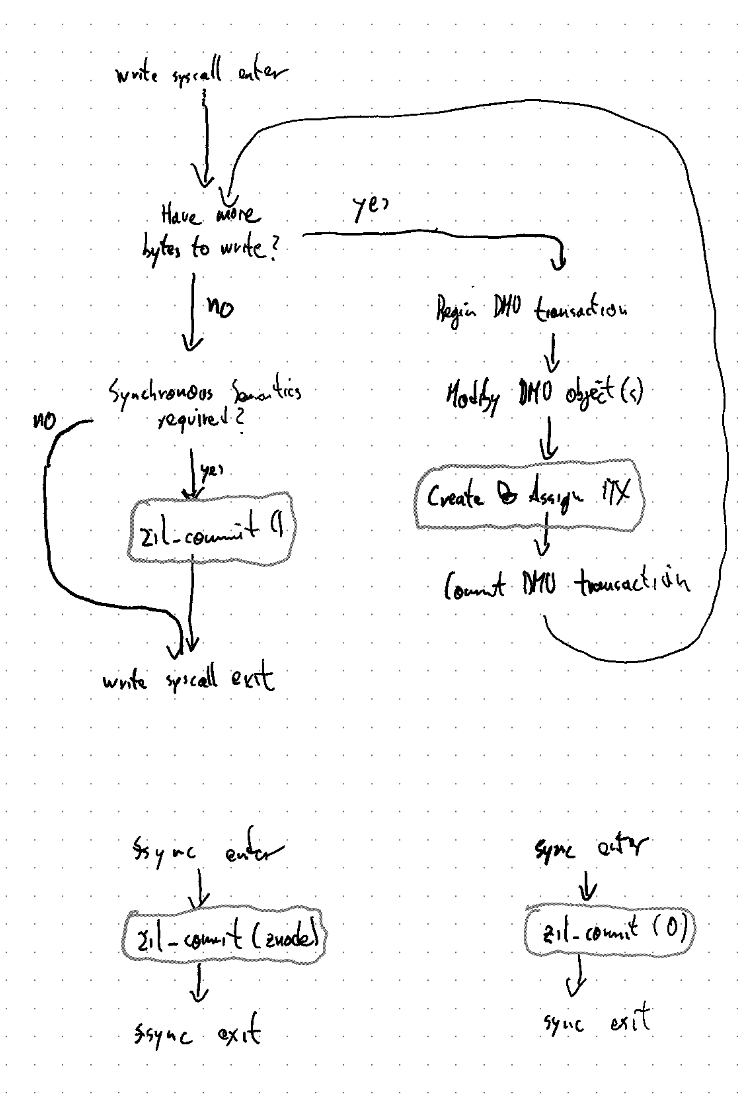
\includegraphics[height=0.8\textheight]{fig/zil_api_syscall_activity_diagram}
    \caption{
        ZIL API usage on the write path in \lstinline{write()}, \lstinline{fsync()}, and \lstinline{sync()} system calls.
    }
    \label{fig:zil_api_syscall_activity_diagrams}
\end{figure}

\lstinline{zilog_t} tracks assigned ITXs in data structures called \lstinline{itxg}.
There exists one \lstinline{itxg} per unsynced pool transaction group (txg).
When an ITX is assigned to the ZIL in a given txg, it is added to that txg's \lstinline{itxg}.
After the txg sync thread has finished syncing a txg, it frees the corresponding \lstinline{itxg} and all the ITXs in it because the changes they describe are now persisted in the main pool and thus obsolete.

Each \lstinline{itxg} is split into a \textit{sync list} and the \textit{async tree}.
The \textit{sync list} is a simple list of ITXs whereas the \textit{async tree} is a search-tree that maps from object ID to a list of ITXs.
By default, ITXs are added to the \textit{sync list} when assigned to the ZIL.
The \textit{async tree} is only used for ITXs that are scoped to a particular file.
For example, an ITX that logs the creation of a file is added to the \textit{sync list} whereas a write within that file is added to the \textit{async tree}.

\lstinline{zil_commit} uses the \lstinline{itxg}s to build a linear \textit{commit list} of ITXs that it can subsequently persist to stable storage.
The following pseudo-code illustrates the construction of the commit list by \lstinline{zil_commit}.
Figure~\ref{fig:zil_per_itxg_state_example} provides an example for a single transaction group.

\begin{lstlisting}
zil_commit(object_id)
    commit_list := []
    for each unsynced transaction group 'txg':
        itxg <- the itxg for txg
        if object_id == 0:
            append all itxs in itxg.async to itxg.sync
        else:
            append only the itxs in
              itxg.async[object_Id] to itxg.sync
        append itxg.sync to commit_list
    err := persist commit_list
    if err:
        wait until the open txg has synced
    return
\end{lstlisting}

\begin{figure}[H]
    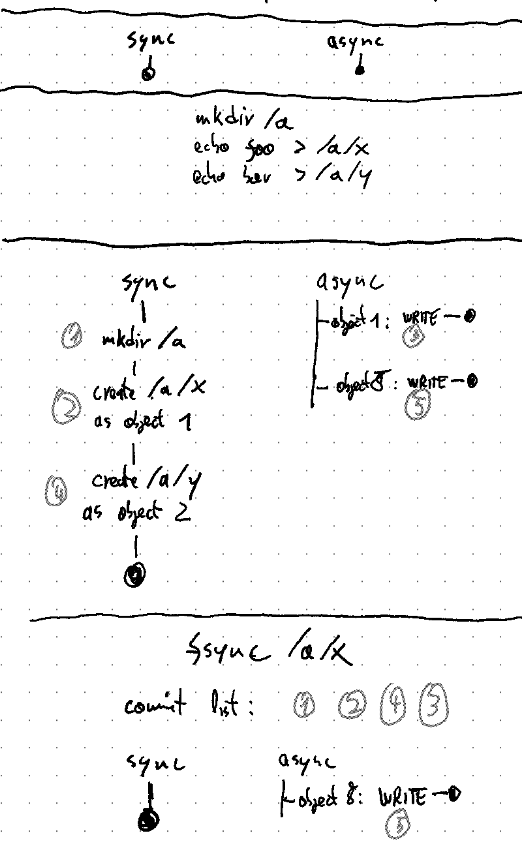
\includegraphics[height=0.5\textheight]{fig/zil_single_itxg_example}
    \caption{
        An example of how an itxg is filled with ITXs and how \lstinline{zil_commit} drains it into a commit list.
        Note that this example only covers the case where all ITXs were assigned for the same txg.
    }
    \label{fig:zil_per_itxg_state_example}
\end{figure}

\subsubsection{zil\_sync}\label{zilsync}
Maybe we can avoid this? It's only relevant in ZIL-PMEM.

\subsection{Replay}


\subsection{Log Record Types}
% \label{wrneedcopy}
% WR\_INDIRECT 

\chapter{ZIL-LWB on PMEM}\label{ch:lwb_analysis}
The motivation for this thesis is the significant overhead of the current ZIL implementation (ZIL-LWB) in 4k random synchronous write workloads compared to the raw PMEM hardware.
In this chapter, we describe this benchmark in detail (Section~\ref{ch:lwb_analysis:setup}) and present the resulting data in Section~\ref{ch:lwb_analysis:results}.
We proceed with an analysis of the distribution of the wall clock time spent during this benchmark among the involved ZFS components.
Our findings (Section~\ref{ch:lwb_analysis:breakdown}) show that approximately 80\% of overall latency are spent on ZIL-LWB-specific code.
We conclude that ZIL-LWB's data structures and persistence mechanisms are unfit to take advantage of PMEM-level performance, motivating the development of ZIL-PMEM.

\section{Benchmark Setup}\label{ch:lwb_analysis:setup}
Our benchmarking system has the following hardware configuration:
\begin{description}[noitemsep,leftmargin=1.5cm,labelindent=1cm]
    \item[CPU] 2 x Intel(R) Xeon(R) Silver 4215 CPU \@ 2.50GHz
    \item[Mainboard] Supermicro X11DPi-N(T)/X11DPi-NT, BIOS 3.1a 10/16/2019
    \item[DRAM] 16 x Micron 8GiB DDR4 2933MT/s (18ASF2G72PDZ-2G9E1), evenly distributed across sockets.
    \item[NVMe] 3 x Micron PRO 960GB NVMe, 512 byte namespace format (MTFDHBA960TDF)
    \item[PMEM] 4 x Intel Optane DC Persistent Memory, 128 GB, (NMA1XXD128GPS), two per socket.
\end{description}
We use the following software stack:
\begin{description}[noitemsep,leftmargin=1.5cm,labelindent=1cm]
    \item[Kernel] Linux 5.9, Debian buster (5.9.0-0.bpo.5-amd64)
    \item[Userland] Debian GNU/Linux (buster)
    \item[fio] fio-3.23-28-g7064
    \item[bpftrace] bpftrace v0.12.0
    \item[bcc] v0.16.0-11-ga74413b0
    \item[OpenZFS] Our tree of OpenZFS with support for \textit{ZIL kinds} (Section~\ref{ch:zilkinds}), configured to use the ZIL-LWB ZIL kind.
        Note that we ensured manually that the \textit{ZIL kinds} patch do not impact ZIL-LWB performance.
\end{description}
We use the following system configuration:
\begin{itemize}[noitemsep]
    \item We leave SMT enabled, resulting in 16 hardware threads per socket.
    \item We disable the entire second CPU in software using the \lstinline{isolcpus=8-15,24-31} kernel command line parameter.
    \item We configure all Optane DIMMs in \textit{AppDirectNotInterleaved} mode.
    \item We create a \SI{40}{GiB}-sized \textit{fsdax} namespace on the region of the first DIMM on the first socket.
    \item We create a \SI{40}{GiB}-sized \textit{devdax} namespace on the region of the first DIMM on the first socket.
    \item We partition the 3 NVMe drives into 10 equals-sized partitions each.
    \item We create a zpool called \texttt{dut} with the 30 partitions as top-level vdevs, and the \texttt{/dev/pmem} device as a SLOG.
        Note that we used the multitude of NVMe partitions because it improvded overall device utilization in our setup.
    \item We create 8 datasets in the zpool, named \lstinline{dut/ds$i} and mounted at \lstinline{/dut/ds$i}.
    \item For all datasets, we configure \lstinline{recordsize=4k} to match the fio workload and set \lstinline{compression=off} to avoid CPU overhead in the ZIO pipeline during \textit{txg sync}.\todo{check defined}
\end{itemize}

We use \textit{fio} to generate a workload of random 4KiB writes with synchronous semantics (\lstinline{blocksize=4k}, \lstinline{rw=randwrite}).
Each of the one to eight \lstinline{numjobs} threads performs random synchronous write system calls to a separate file per thread (\lstinline{ioengine=sync}, \lstinline{sync=1}, \lstinline{direct=0}, \lstinline{fsync=0}).
Each file has a size of \lstinline{size=100MiB} which means that the written data volume grows with \lstinline{numjobs}, but the amount of dirty data (max.\SI{800}{MiB}) remains well below the NVMe drive's bandwidth limits.
To avoid scalability-bottlenecks in the \lstinline{itxg} layer\todo{check this is defined}, we place each thread's file onto a separate dataset \lstinline{/dut/ds$jobnum/fio_file} using the \lstinline{filename_format} option.
For each value of \lstinline{numjobs}, we measure for one minute (\lstinline{time_based=1}, \lstinline{runtime=60}), with a ramp-up time of \SI{2}{seconds} (\lstinline{ramp_time=2}), and set \lstinline{end_fsync=1}.
Before we run the benchmark, we prepare the benchmark files with a separate fio invocation with the additional flag \lstinline{--create_only=1}.

We apply the fio workload to the following storage stacks:
\begin{description}[noitemsep,leftmargin=1.5cm,labelindent=1cm]
    \item[zil-lwb] The zpool with ZIL-LWB ZIL kind as described above.
    \item[async] The same configuration as above, but with \lstinline{sync=disabled} set on all datasets.
        This turns \lstinline{zil_commit} into a no-op, reducing the time spent in the \lstinline{write} system call to DMU object modification and ITX allocation, all in DRAM.
    \item[fsdax] The fio configuration above, applied directly to the \texttt{/dev/pmem} block device (\lstinline{direct=1} instead of \lstinline{direct=0}, and \lstinline{filename=/dev/pmem0} instead of \lstinline{filename_format=...}).
        This configuration demonstrates the performance of the Linux block device emulation around the PMEM hardware. It includes the syscall overhead.
    \item[devdax] The fio configuration above, with \lstinline{ioengine=dev-dax}, applied directly to the \texttt{/dev/dax} namespace (\lstinline{filename=/dev/dax0.1} instead of \lstinline{filename_format=...}).
        In this configuration, fio mmaps the PMEM namespace directly and thus bypasses the kernel completely.
\end{description}

% \begin{description}
%     \item[ioengine] sync
%     \item[end_fsync] 1
%     \item[size] 100MiB
%     \item[blocksize] 4k
%     \item[rw] randwrite
%     \item[time\_based] 1
%     \item[runtime] 60 seconds
%     \item[ramp\_time] 2 seconds
%     \item[sync] 1
%     \item[direct] 0
%     \item[fsync] 0
%     \item[numjobs] We vary this variable from 1 to 8.
%     \item[group_reporting] 1
% \end{description}

\section{Results}\label{ch:lwb_analysis:results}

The following graphs show the achieved IOPS and per-thread latency by numjobs.

\begin{figure}[H]
    \centering
    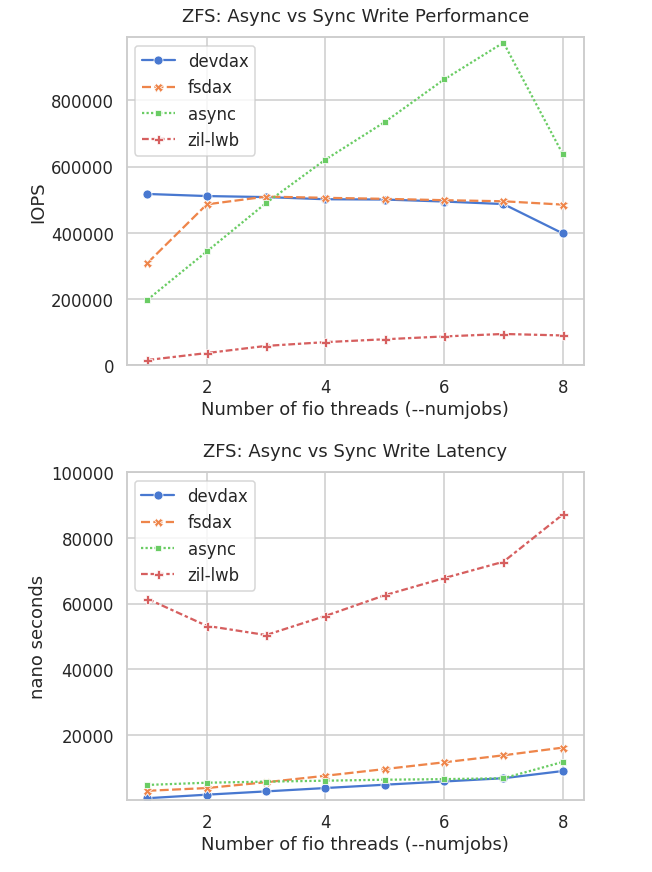
\includegraphics[height=14cm]{fig/evaluation/motivating_fio_benchmark__iops_and_latency.png}
    \caption{IOPS and latency ZIL-LWB compared to ZFS in async mode as well as the raw fsdax and devdax device.}
    \label{fig:lwbanalysis:iops_and_latency}
\end{figure}

ZIL-LWB only achieves approximately 10k IOPS at one thread and peaks at approximately 100k IOPS at seven threads.
In contrast, ZFS in \textit{async} mode starts with 200k IOPS with one thread and achieves over 900k IOPS at seven threads.
This exceeds the performance of the PMEM hardware which mostly stays at 500k IOPS and demonstrates that the ZIL is clearly the bottleneck in the \textit{zil-lwb} configuration.
A look at the per-IOP average latency emphasizes the vast overhead that ZIL-LWB adds compared to what is possible with the raw PMEM hardware.
Whereas ZFS in async mode only requires \SI{5}{us} per IOP with \lstinline{numjobs=1}, and raw writes to fsdax require approximately \SI{3}{us}, ZIL-LWB with the same PMEM hardware as SLOG takes more than \SI{60}{us} per write.
The minimum latency achieved by ZIL-LWB is at \lstinline{numjobs=4} at approximately \SI{50}{us} before it starts increasing to up to approximately \SI{85}{us} at \lstinline{numjobs=8}.
Note that we do not use the results from the \textit{dev-dax} as a baseline for PMEM hardware because the IOPS and latencies reported by fio do not match.
For example, fio reports less than \textit{dev-dax} \SI{1}{us} of latency for \textit{dev-dax} but only reports 550k IOPS at \lstinline{numjobs=1} whereas $\frac{1}{\SI{1}{us/IOPS}} = 10^6~\si{IOPS}$ would be anticipated at this latency.
Figure~\ref{fig:lwbanalysis:zoomed_latency} shows the same latency data as Figure~\ref{fig:lwbanalysis:iops_and_latency} above, albeit zoomed to a scale that allows us to distinguish \textit{dev-dax}, \textit{fsdax}, and \textit{async} latencies.

\begin{figure}[H]
    \centering
    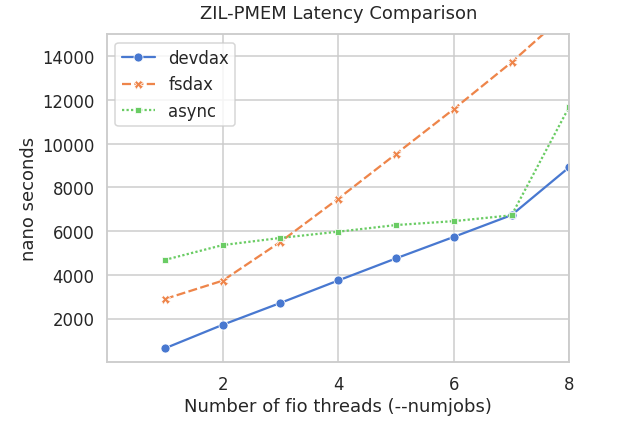
\includegraphics[height=7cm]{fig/evaluation/motivating_fio_benchmark__latency_zoomed.png}
    \caption{Zoomed section of Figure~\ref{fig:lwbanalysis:iops_and_latency} that allows us to distinguish async mode, devdax, and fsdax.}
    \label{fig:lwbanalysis:zoomed_latency}
\end{figure}

\section{Analysis}\label{ch:lwb_analysis:breakdown}

By comparing the numbers for \textit{async} and \textit{zil-lwb}, it is safe to assume that regardless of the value for \lstinline{numjobs}, ZIL-LWB adds at least \SI{40}{us} of latency.
We want to determine where this time is spent.

\subsection{OpenZFS Background: How ZIL-LWB Works}\label{ch:lwb_analysis:openzfs_background_zil_lwb}
We have introduced the DRAM representation of the ZIL in Section~\ref{openzfs:the_zil_api}:
Syscalls modify DMU objects in so-called DMU transactions and log the logical change made in a transaction as an ITX to the ZIL.
The ZIL stores the ITXs in a data structure called \textit{itxg} until either the transaction group of the ITX's DMU transaction is synced to disk or synchronous semantics are requested through \lstinline{zil_commit}.
In the latter case, the ZIL constructs the \textit{commit list} which is the sequence of ITXs that needs to be concatenated to some form of per-dataset persistent log structure before \lstinline{zil_commit} is allowed to return.

ZIL-LWB uses a chain of so-called \textit{log-write blocks} (LWBs) to represent this log structure.
The LWB chain is a single-linked list rooted in the ZIL header of each dataset.
Each LWB contains a contiguous sequence of variable-length \textit{log records}.
A log record is the persistent representation of an ITX.
To reconstruct the concatenated commit lists, ZIL-LWB traverses the LWB chain and concatenates the log record sequences within the LWBs.
Figure~\ref{fig:zil_lwb__physical_structure_overview} visualizes this structure.

\begin{figure}[H]
    \centering
    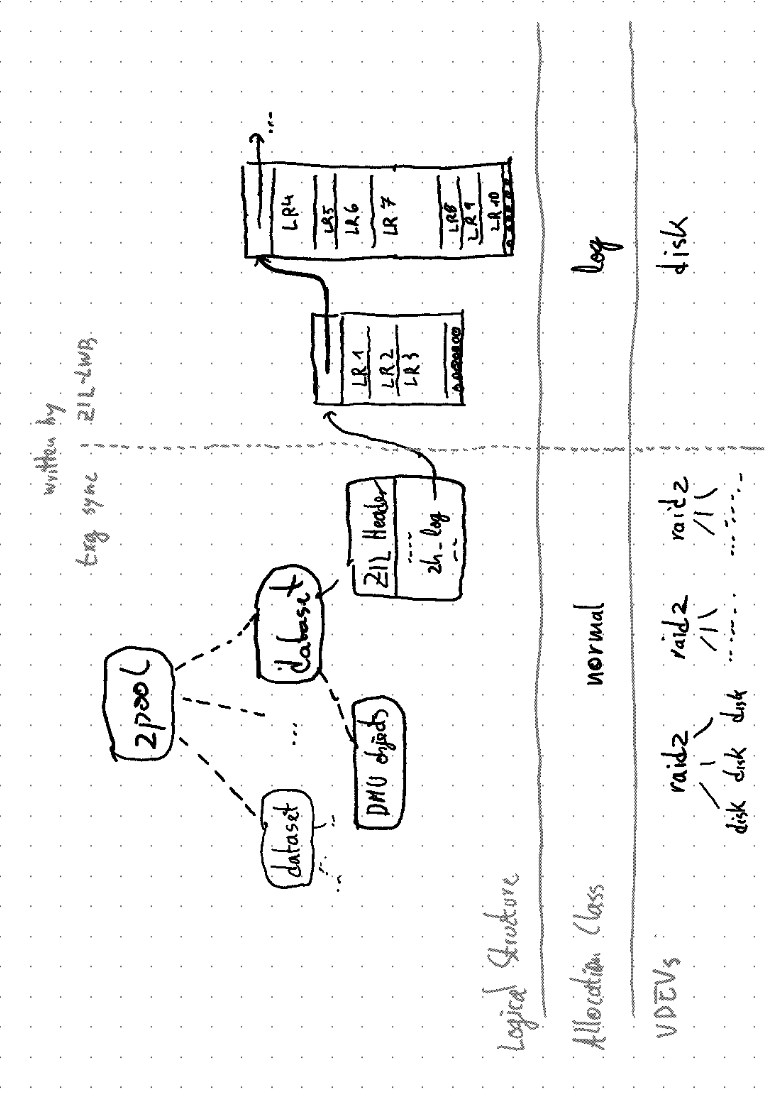
\includegraphics[height=\textwidth,angle=270]{fig/zil_lwb__physical_structure_overview}
    \caption{On-disk structure of ZIL-LWB as described in the previous paragraph.}
    \label{fig:zil_lwb__physical_structure_overview}
\end{figure}

The packing of $N$ log records on the commit list into $M$ larger LWBs has been advantageous in the past:
\begin{description}[noitemsep]
    \item[Latency Amortization]
        Under the assumption that disk latency ($lat_{disk}$) dominates overall synchronous I/O latency, writing log records one-by-one would result in a total latency of $N * lat_{disk}$.
        In contrast, grouping records into $M << N$ LWBs reduces the latency to $M * lat_{disk}$
    \item[LWB Timeout / Group Commit]
        ZIL-LWB uses a \textit{timeout} mechanism to extend the amortizing effect of LWB packing.
        When a thread $A$ packs log records into LWBs, it issues the IO operations for all but the last LWB as soon as the LWB is filled.
        The last LWB remains in \textit{open} state for a short time window.
        If another thread $B$ \lstinline{zil_commit}ting to the same dataset within that time window, it picks up the \textit{open} LWB and continues to fill it with log records from its own \textit{commit list} and issues the LWB IO operation as soon as the LWB is full.
        The IO completion callback then wakes up $A$ and which can now safely return from \lstinline{zil_commit} because $A$'s commit list is now fully persisted.
        If the LWB is not committed within the configured time window, $A$ issues the IO operation itself.
        Without the timeout mechanism, thread $B$ would need to wait for the last LWB of $A$ to be persisted, \textit{and} for its own LWBs to be persisted because $B$'s first LWB is pointed to by $A$'s last LWB.
        By sharing the last LWB of $A$ and $B$, up to $1 * lat_{disk}$ of waiting time can be avoided.\todo{review this, just thought of it}
        Note that whereas ZFS refers to this mechanism as \textit{LWB timeout}, the technique is also well-established in disk-oriented databses under the term \textit{group commit} or \textit{commit group}.
    \item[Space Efficiency]
        Log records are stored as a contiguous sequence within the LWB.
        This avoids fragmentation if the commit list consists of small log records because many such log records can be packed into the smallest LWB (\SI{4}{KiB}).
        However, the on-disk format does not allow for splitting of individual log records.
        If the log record cannot be split in software (\lstinline{WR_NEED_COPY}), the open LWB is issued with wasted space and a new LWB is allocated for the log record.
\end{description}

LWBs are allocated from the metaslab allocator which identifies the location of allocated data through a \textit{ZFS block pointer}.
Block pointers are fat pointers (\SI{128}{byte}) that, among other metadata, contain up to three \textit{data virtual addresses} (DVAs) that identify where one to three copies of the data are stored.
A DVA consists of the top-level vdev ID and an offset in the vdev's logical block address space --- other systems would probably refer to this as logical extent(s).
Block pointers also store the checksum of the data that they point to.
Computing this checksum is possible because ZFS's main on-disk structure is a tree that is written bottom-up by the \textit{txg sync} thread for every transaction group.
The end result is a merkle tree that is rooted in a block pointer stored in ZFS's \textit{uberblock} which is roughly equivalent to superblocks in other filesystems.

The LWB chain is a special case because the ZIL must be able to add new LWBs between transaction groups.
The solution is to pre-allocate LWBs and to store the checksum of their content in the LWB itself.
The procedure to write out an LWB thus is as follows:
\begin{enumerate}[noitemsep]
    \item Wait until the LWB is filled or the timeout triggers the LWB to be written out.
    \item Predict the best size for the next LWB based on a simple heuristic.
    \item Allocate the next LWB, prerrably from the \textit{log} allocation class.
    \item Store the resulting block pointer in the current LWB so that it points to the next LWB.
    \item Compute the checksum of the current LWB.
    \item Repurpose the current LWB's block pointer field to store the computed checksum.
    \item Write out the current LWB.
\end{enumerate}
Figure~\ref{fig:zil_lwb__physical_structure_append} visualizes these steps for the initial case where no log exists, and for an existing log.
The LWB chain's end is implicitly marked by an invalid checksum.
The checksum also ensures crash-consistency since the list is append-only and a partially written block is equivalent to the end of the log during recovery.
Note that it is unlikely for an unwritten but allocated LWB to be mistaken for a valid LWB block due to additional metadata stored in the LWB.
For OpenZFS native encryption, the LWBs are not checksummed but encrypted and authenticated using an AEAD algorithm\todo{I think cipher mode is not the right term} such as \lstinline{aes-256-gcm}.

\begin{figure}[H]
    \centering
    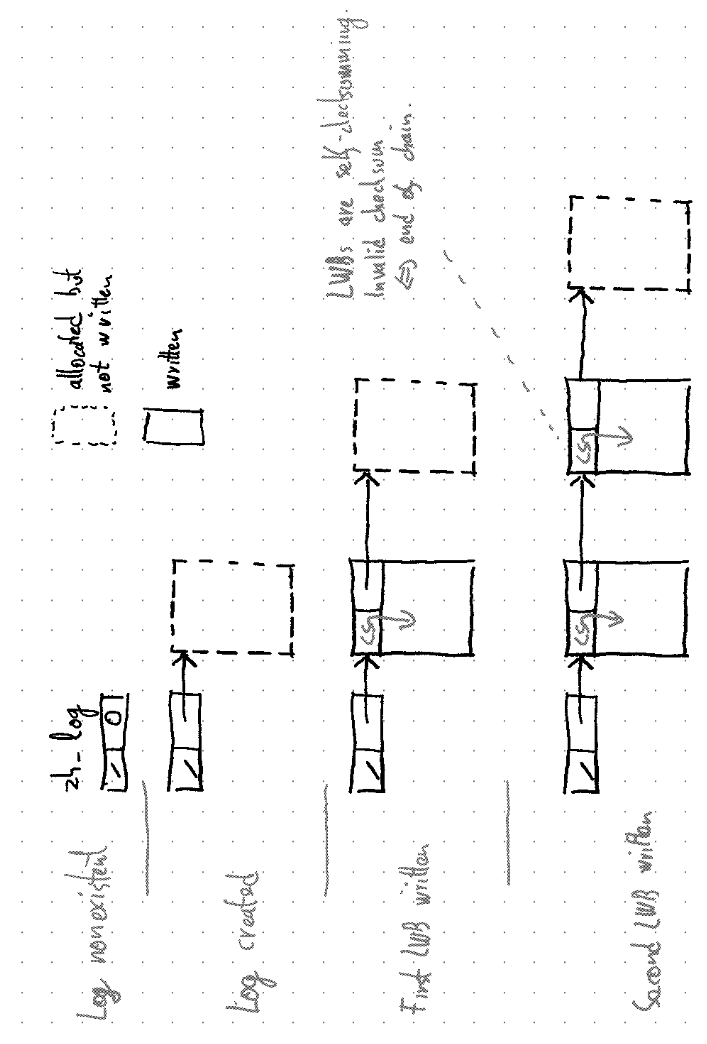
\includegraphics[height=\textwidth,angle=270]{fig/zil_lwb__physical_structure_append.png}
    \caption{The procedure for appending an LWB.}
    \label{fig:zil_lwb__physical_structure_append}
\end{figure}

ZIL-LWB does not write LWBs directly using the kernel's block device API but uses the ZFS \textit{ZIO pipeline} instead.
ZIO is ZFS's unified abstraction for performing deferred allocation, transparent data and metadata checksumming, compression, deduplication and encryption as well as redundancy mechanisms such as raidz.
The architecture is pipeline-oriented and heavily parallelized using ZFS's \textit{taskq}s to maximize throughput for its main consumer, \textit{txg sync}.
By using the same infrastructure for LWB ZIO operations, a very high degree of code reuse is possible, although there are some special cases, in particular for self-checksumming or encryption.
Also, integrating LWB I/O into the ZIO pipeline could be beneficial for the case where the pool does not have a SLOG configured because latency-sensitive ZIO operations can be prioritized over throughput-oriented \textit{txg sync} operations.
However, as we will elaborate on in the next subsections, ZIO adds significant latency overheads, resulting in sub-par performance of ZFS on low-latency storage devices, and PMEM in particular.

\subsubsection{Analysis}

Given the background knowledge on how ZIL-LWB works, we are now ready to present out latency analysis.
We use dynamic instrumentation (eBPF via bpftrace\todo{cite}) to sum up the wall clock time spent in ZFS functions that are executed by the fio threads during a synchronous write.
We then use the model in Figure~\ref{fig:lwbanalysis:breakdown_model} to compute the time spent in the asynchronous part of the write operation, the ITX layer, and ZIL-LWB specific code.
We visualize the results as stacked bar charts in Figure~\ref{fig:lwbanalysis:breakdown_charts}.

\begin{figure}[H]
    \centering
    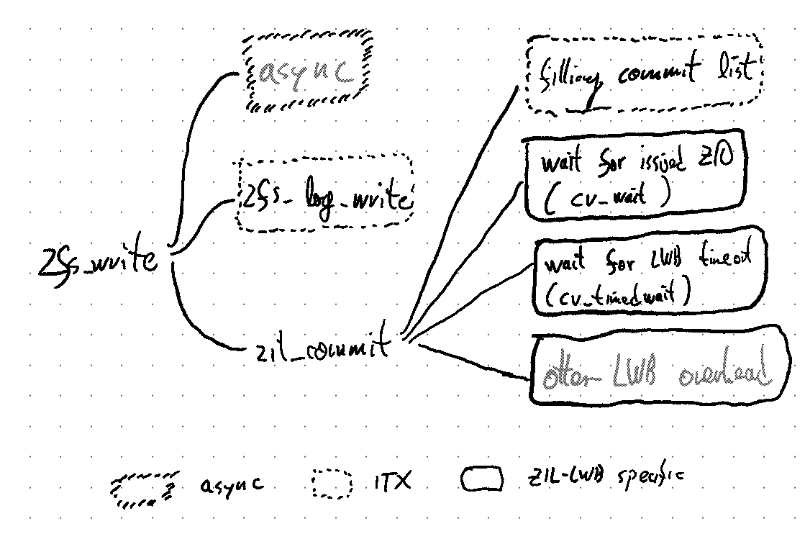
\includegraphics[height=6cm]{fig/zil_lwb_latency_analysis__breakdown}
    \caption{Our model of the time spent in ZFS by a fio thread that performs a write system call.
    The different colums represent the different levels of the dynamic call graph
    The nodes in each column describe all activity that happens at this level of the call graph.
    Activities with black text color are instrumented using eBPF.
    Gray text color indicates that the value was computed in post-processing by subtracting the sum of the columns instrumented time from the instrumented time of the parent in the column to the left.
    For example, to compute \textit{async}, we compute \lstinline{zfs_write - (zil_commit + zfs_log_write)}.
    The border style of the node visualizes the subsystem to which we attribute the time spent in the activity represented by the node.
    }
    \label{fig:lwbanalysis:breakdown_model}
\end{figure}

\begin{figure}[H]
    \centering
    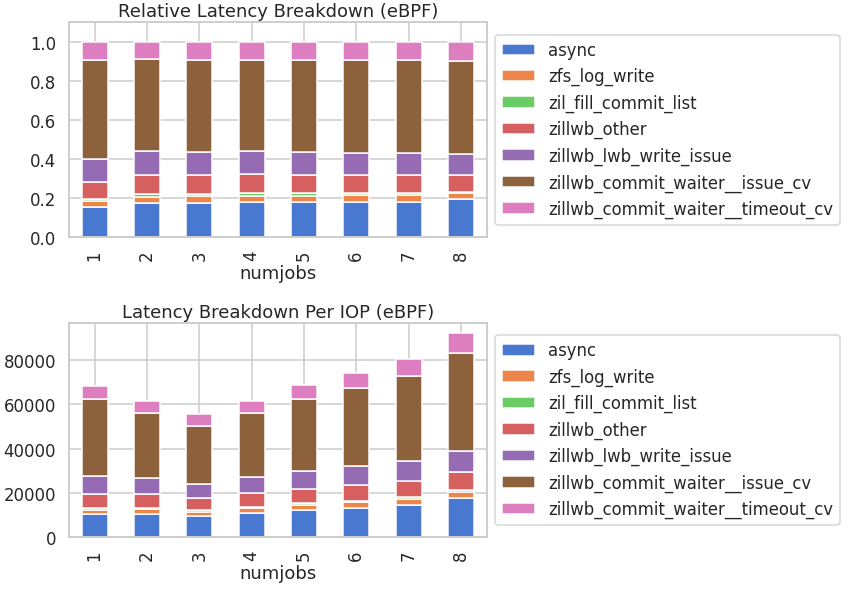
\includegraphics[height=10cm]{fig/evaluation/zillwb_latency_analysis__relative_and_absolute_latency_breakdown}
    \caption{The relative and absolute breakdown of latency by activity.
    The absolute breakdown is normalized by the number of write operations.
    We compared the latencies in the breakdown with the latencies observed by fio to ensure that our accounting is correct under the given model.
    }
    \label{fig:lwbanalysis:breakdown_charts}
\end{figure}

Our observations are as follows:
\begin{itemize}[noitemsep]
    \item The instrumentation overhead is 5--\SI{10}{us} per IOP. (We compared the latencies that fio reports for the instrumented and uninstrumented run.)
    \item The relative distribution of latency remains mostly unchanged for the different values of \lstinline{numjobs}.
    \item The \textit{async} part of the write path and the ITX layer together only amount to approximately 20\% of overall latency.
        The remaining 80\% are spent on LWB-specific activities.
    \item The LWB timeout mechanism amounts to 4\% of overall latency.
    \item At least 20\% of overall latency are spent on filling LWBs, issuing their corresponding ZIOs, and other LWB-related activities.
    \item 45--50\% of overall latency is spent waiting for the ZIO pipeline to persist the LWBs.
        In absolute numbers, the value ranges from 25--\SI{40}{us}.
        We have separately confirmed that ZIL-LWB uses \SI{12}{KiB} LWBs which is the smallest possible LWB size allowed by the implementation.
        In our benchmarking setup (per-thread datasts), each LWB only holds a single \SI{4}{KiB} write log record with \SI{192}{B} of additional metadata.
        This amounts to write amplification of 3x.
        However, even with this increased data volume per IOP, the results from the previous experiment suggest that with a conservative estimate of \SI{3}{us} per 4k write to the raw PMEM hardware, we should expect less than \SI{9}{us} of PMEM write time per LWB.
        Thus, a major fraction of the 25--\SI{40}{us} that are spent waiting for ZIO is actually pure software overhead.
\end{itemize}

Our observations lead us to the following conclusions:

\textbf{First, we have reason to believe that the high overhead of ZIO is unlikely to be reduced} to a degree that allows for exploitation of PMEM-level latency, regardless of whether the hardware is actual PMEM or simply very fast NVMe drives.
The reason is that there is an inherent conflict of goals for ZIO:
whereas the ZIL is strictly latency-oriented, all other conumers (\textit{txg sync}, \textit{scrubbing}, \textit{zfs send/recv}) are throughput-oriented.
The pipeline-oriented, parallelized architecture of ZIO is important for throughput and provides great flexibility, but increases latency through context switches.
This problem is well known in the ZFS community, see \cite{openzfsZILPerformanceImprovements2020}.\todo{more quotes, find gh issues, etc}

\textbf{Second, the persistent representation of the ZIL as a chain of LWBs poses a severe and unnecessary overhead on PMEM.}
For one, the latency amortization provided by LWBs and the timeout mechanism is unnecessary at PMEM-level latencies where it is cheaper to persist the log records on an individual basis than batching them in LWBs and coordinating with other threads on the matter.
And for another, since PMEM is byte-addressable, the persistent representation is no longer constrainted by disk block sizes, opening up the possibility of better space efficiency.

\chapter{Design Overview}\label{ch:designoverview}
Given the insights described in the previous chapter, we propose an alternative ZIL implementation called \textbf{ZIL-PMEM} that exclusively targets PMEM SLOG devices.
In this chapter we define the project goals for ZIL-PMEM and provide a high-level overview of its design.
The subsequent two chapters then introduce the core data structure and our approach to integrating it into ZFS.

\section{Project Goals \& Scope}

\newcommand{\csgoal}[1]{\textbf{#1}}

\subsection{Requirements}\label{sec:requirements}

\csgoal{Coexistence}
ZIL-PMEM must coexist with ZIL-LWB in code and at runtime due to limited availability of PMEM hardware and the limitations of the ZIL-PMEM design.

\csgoal{Same Guarantees}
ZIL-PMEM must maintain the same crash consistency guarantees towards user-space as ZIL-LWB for both ZPL and ZVOL.

\csgoal{Simple Administration \& Pooled Storage}
Pooling of storage resources and simple administration are central to ZFS~\cite{bonwickZettabyteFileSystem2003}.
ZFS should automatically detect that a SLOG device is PMEM and, if so, use ZIL-PMEM for all of the pool’s datasets.
No further administrative action should be required to fully benefit from ZIL-PMEM.

\csgoal{Correctness}
In the absence of PMEM media errors and data corruption, ZIL-PMEM must be able to replay all data that it reported as committed.
The result must be the same as if ZIL-LWB would have been used in lieu.
Specifically:
\begin{itemize}[noitemsep,beginpenalty=100000,midpenalty=100000]
    \item Replay must respect the logical dependencies between log records.
    \item Logging must be crash-consistent, i.e., the in-PMEM state must always be such that replay is correct.
    \item Replay must be crash-consistent, i.e., if the system crashes or loses power during replay, it must be possible to resume replay after the crash.
        Resumed replay must continue to respect logical dependencies of log records.
\end{itemize}

\csgoal{Data Integrity}
Data integrity is a core feature of ZFS~\cite{bonwickZettabyteFileSystem2003}.
ZIL-PMEM must detect corrupted log records using an error-detecting code.
Detected corruption must be handled \textit{correctly} (as outlined in the previous paragraph) and \textit{gracefully} with the following behavior as the baseline:
``Assume a sequence of log records $1 \dots N$ where log record $1$ does not depend on a log record and each record $i > 1$ depends on its predecessor $i-1$.
Data corruption in record $i \in 1 \dots N$ must not prevent replay of records $1 \dots i-1$".

\csgoal{Low Latency}
The latency overhead of ZIL-PMEM compared to raw PMEM device latency for the same data volume should be minimal for single-threaded workloads.
Multi-threaded workloads are addressed below.

\csgoal{Multi-Core Scalability}
Since PMEM is added as a pool-wide resource used by all of the pool's datasets, ZIL-PMEM should scale well to multiple cores.
Barring PMEM throughput limitations, the speedup in throughput (IOPS) achieved by parallelizing synchronous I/O to multiple cores on a ZIL-PMEM system should be as follows:
{
\setlength{\parskip}{0pt}
\begin{description}[topsep=0pt, noitemsep, leftmargin=1cm, labelindent=1cm, widest=1 private dataset per thread]
    \item[1 private dataset per thread] Always near-linear speedup.
    \item[1 shared dataset] \mbox{}
          \begin{description}[noitemsep, leftmargin=1cm, labelindent=1cm, widest=ZPL filesystem]
              \item[ZPL filesystem] No speedup.
              \item[ZVOL] No speedup in standard mode, potentially sub-linear speedup in bypass mode (Section~\ref{sec:itxgbypass}).
          \end{description}
\end{description}
}

\csgoal{Maximum Performance On Intel Optane DC Persistent Memory}
We develop and evaluate ZIL-PMEM exclusively for/on Intel Optane DC Persistent Memory since it is the only broadly available non-volatile main memory product on the market.
Whereas supercapacitor-backed persistent memory modules (NVDIMM-N) should be usable with ZIL-PMEM, our goal is to design a system that makes optimal use of the Optane hardware.

\csgoal{CPU-Efficient Handling Of PMEM Bandwidth Limits}
If the maximum write bandwidth to any kind of storage device is exceeded, the I/O stack must somehow apply back-pressure to avoid losing in-flight data.
With PMEM, the I/O stack is the CPU microarchitecture and the back-pressure manifests as stalling instructions.
However, from the OS thread scheduler's perspective, threads whose instructions stall because they wait for PMEM are indistinguishable from actually busy threads.
\citeauthor{yangEmpiricalGuideBehavior2020} have shown that a single Optane DIMM's write bandwidth can be exhausted by one CPU core at \SI{2}{GB/s} and that write bandwidth decreases to \SI{1}{GB/s} at ten or more CPU cores.
% In contrast, DRAM shows a near-linear increase in bandwidth to \SI{60}{GB/s} at 15~threads.~\cite[fig.4]{yangEmpiricalGuideBehavior2020}
Since ZIL-PMEM shares PMEM among all datasets in a zpool, we expect bandwidth exhaustion to be a phenomenon that wil happen in practice.
ZIL-PMEM should thus provide a mechanism to shift excessive PMEM I/O wait time off the CPU.

\csgoal{Testability}
ZIL-PMEM must be architected for testability.
The core algorithms must be covered by unit tests.
Further, ZIL-PMEM should be integrated into the ztest user-space stress test as well as the SLOG tests of the ZFS Test Suite.

\subsection{Out Of Scope For The Thesis}
The following features were omitted to constrain the scope of the thesis.
We believe that our design can accomodate them without major changes.

\csgoal{Support For OpenZFS Native Encryption}
The ZIL-PMEM design presented in this section does not address OpenZFS native encryption.
Intel Optane DC Persistent Memory supports transparent hardware encryption per DIMM at zero overhead\todo{cite spec}.
In contrast, OpenZFS native encryption is per dataset and software-based.
Given these significant differences in data and threat model, ZIL-PMEM cannot rely on Optane hardware encryption.
Instead, ZIL-PMEM would need to invoke OpenZFS native encryption and decryption routines when writing or replaying log entries.

\csgoal{Protection Against Scribbles}
Scribbles are bugs in the system that accidentally overwrite PMEM, e.g., due to incorrect address calculation or out-of-bounds access in the kernel.
PMEM-specific filesystems such as PMFS and NOVA-Fortis have already introduced mechanisms to protect againt scribbles~\cite{dulloorSystemSoftwarePersistent2014,xuNOVAFortisFaulttolerantNonvolatile2017}.
We believe that these mechanism can be applied to our design as well.

\subsection{Limitations}
The following features are deliberately not addressed by our design.
More experimentation and experience with ZIL-PMEM will benecessary to determine which features are useful in practice, how they can be realized, and how they interact with the existing requirements.

\csgoal{No NUMA Awareness}
\citeauthor{yangEmpiricalGuideBehavior2020} recommend to ``avoid mixed or multi-threaded accesses to remote NUMA nodes. [...]  For writes, remote Optane’s latency is 2.53x (ntstore) and 1.68x higher compared to local"~\cite{yangEmpiricalGuideBehavior2020}.
We do not account for this behavior in the design and do not evaluate ZIL-PMEM in a NUMA configuration.\todo{future work}

\csgoal{No Data Redundancy}
ZIL-PMEM provides data integrity protections but does not provide a mechanism for data redundancy.\todo{future work}

\csgoal{Only Works With SLOGs}
Our approach to integrate ZIL-PMEM into ZFS is only applicable to PMEM SLOGs and does not work for a zpool that uses PMEM as main pool vdevs.
Such pools continue to use ZIL-LWB.

\csgoal{No Software Striping}
Our design only supports a single PMEM SLOG device.
Users may wish to use multiple PMEM DIMMs to increase log write bandwidth.
With Intel Optane DC Persistent Memory, multiple PMEM DIMMs can be interleaved in hardware with near-linear speedup~\cite{yangEmpiricalGuideBehavior2020}.
Whereas software striping would be the natural approach to ZFS, it will be non-trivial to achieve the same speedup as hardware-based interleaving.

\csgoal{No Support For \lstinline{WR_INDIRECT}}
ZIL-LWB writes the data portion of large write log records directly to the main pool devices.
The ZIL record then only contains metadata such as \lstinline{mtime} and a block pointer to the location in the main pool.
This technique avoids double-writes which is particularly advantageous if the pool does not have a SLOG, which in turn is a use case that ZIL-PMEM does not address (see above).
Further, if a SLOG is available, \lstinline{WR_INDIRECT} log record write latency is likely to be dominated by the main pool's IO latency if it consists of regular block devices.
If the main pool's IO latency were acceptable, a fast NVMe-based ZIL-LWB SLOG or no SLOG at all would likely be sufficient for the setup in question.

\csgoal{Space Efficiency}
ZIL-PMEM is allowed to trade PMEM space for time and simplicity when presented with the option.
Our justification is twofold.
First, PMEM capacities are significantly higher than DRAM.
For example, the smallest Intel Optane DC Persistent Memory DIMM offered by Intel is \SI{128}{GiB}.~\cite{optanepricing_missing}
Second, the maximum amount of log entry space required from any ZIL implementation is a function of the maximum amount of dirty data allowed in the zpool.\todo{ref background section? this sentence should remain, though}
For ZIL-LWB, small SLOG devices of \SI{16} to \SI{32}{GiB} are sufficient in practice.\todo{ref ix systems truenas M}
Thus, there is sufficient headroom for PMEM space usage in ZIL-PMEM.

\section{Design Overview}\label{sec:designoverview}
We introduce the concept of \textit{ZIL kinds} to ZFS.
The ZIL kind is a pool-scoped variable that determines the pool's strategy for persisting ZIL entries.
A zpool's ZIL kind is determined by the following rule:
if the pool has exactly one SLOG and that SLOG is PMEM, the ZIL kind is ZIL-PMEM. Oterwise, it is ZIL-LWB.
As explained in Section~\ref{ch:lwb_analysis:openzfs_background_zil_lwb}, ZIL-LWB uses ZFS's metaslab allocator to allocate log-write blocks (LWBs) from the storage pool with a bias towards SLOG devices.
In contrast, ZIL-PMEM disables metaslab allocation for the PMEM SLOG device and uses the PMEM space directly.

Ee partition the PMEM SLOG's space into fixed-size contiguous segments called \textit{chunks}.
We develop a data structure called \textit{PRB} that consumes theses chunks and exposes the abstraction of an unordered persistent storage layer for \textit{log entries}.
A log entry is the unit of data that can be written to and read from PRB.
It consists of the the ZIL's log \textit{record} and PRB-specific metadata.
PRB scales to many concurrent writers and features a mechanism to avoid excessive on-CPU waiting for PMEM I/O.
Log entries stored in PRB are automatically garbage-collected when they become obsolete because their transaction group has been synced.

PRB provides a pool-wide storage substrate for log entries but does not define any structure.
This is the role of the \textit{HDL} abstraction which implements a mostly sequential log structure on top of PRB.
Each dataset in the zpool has a separate HDL to which it writes log entries.
The HDL adds metadata to the entry that attributes it to the HDL and encodes the log's structure.
After a system crash, the HDLs scan PRB for entries that need to be replayed and \textit{claim} them to hold them back from garbage collection.
For replay, the HDL API provides a callback-based interface that allows its consumer to apply the changes that are encoded in the log entries in sequential, deterministic order.
Loss of entries, e.g., due to data corruption, is handled as gracefully as possible under the constraints of the logical dependencies encoded in the log structure.

Pools of the ZIL-PMEM ZIL kind use PRB/HDL to persist ZIL log records.
For this purpose\todo{language}, we refactor the existing \textit{zil.c} code module.
Before the introduction of ZIL kinds, the struct \lstinline{zilog_t} implemented all ZIL-related functionality.
With ZIL kinds, \lstinline{zilog_t} acts as an abstract base class that encapsulates shared ZIL functionality.
This includes the definitions of the ZIL log record format and the \textit{itxg} data structure that tracks which log entries need to be persisted when synchronous semantics are requested by a syscall.
% % for a whole dataset (\lstinline{sync()}), a single file (\lstinline{fsync()}) or an individual syscall (e.g. \lstinline{write()} on an \lstinline{O_SYNC} file descriptors).
The code that is responsible for persisting log entries resides in ZIL-kind-specific subclasses.
The pool's ZIL kind determines which subclass is instantiated at runtime.
The subclass for ZIL-LWB is \lstinline{zilog_lwb_t} which contains the original LWB code that we move from \textit{zil.c} into the new \textit{zil\_lwb.c} module.
The subclass for ZIL-PMEM is \lstinline{zilog_pmem_t}.
It is a thin wrapper around HDL's methods for writting and replaying log entries.
\lstinline{zilog_pmem_t} is implemented in the \textit{zil\_pmem.c} code module.
This module also contains the code that sets up PRB/HDL on top of the PMEM SLOG vdev, and the code that synchronizes the lifecylces of HDLs their corresponding datasets.

The next two\todo{check} chapters describe our design in detail.
Chapter~\ref{ch:prbhdl} describes our main contribution --- the PRB/HDL data structure.
The integration of PRB/HDL into ZFS is then presented in Chapter~\ref{ch:zilpmem}.

\begin{figure}[H]
    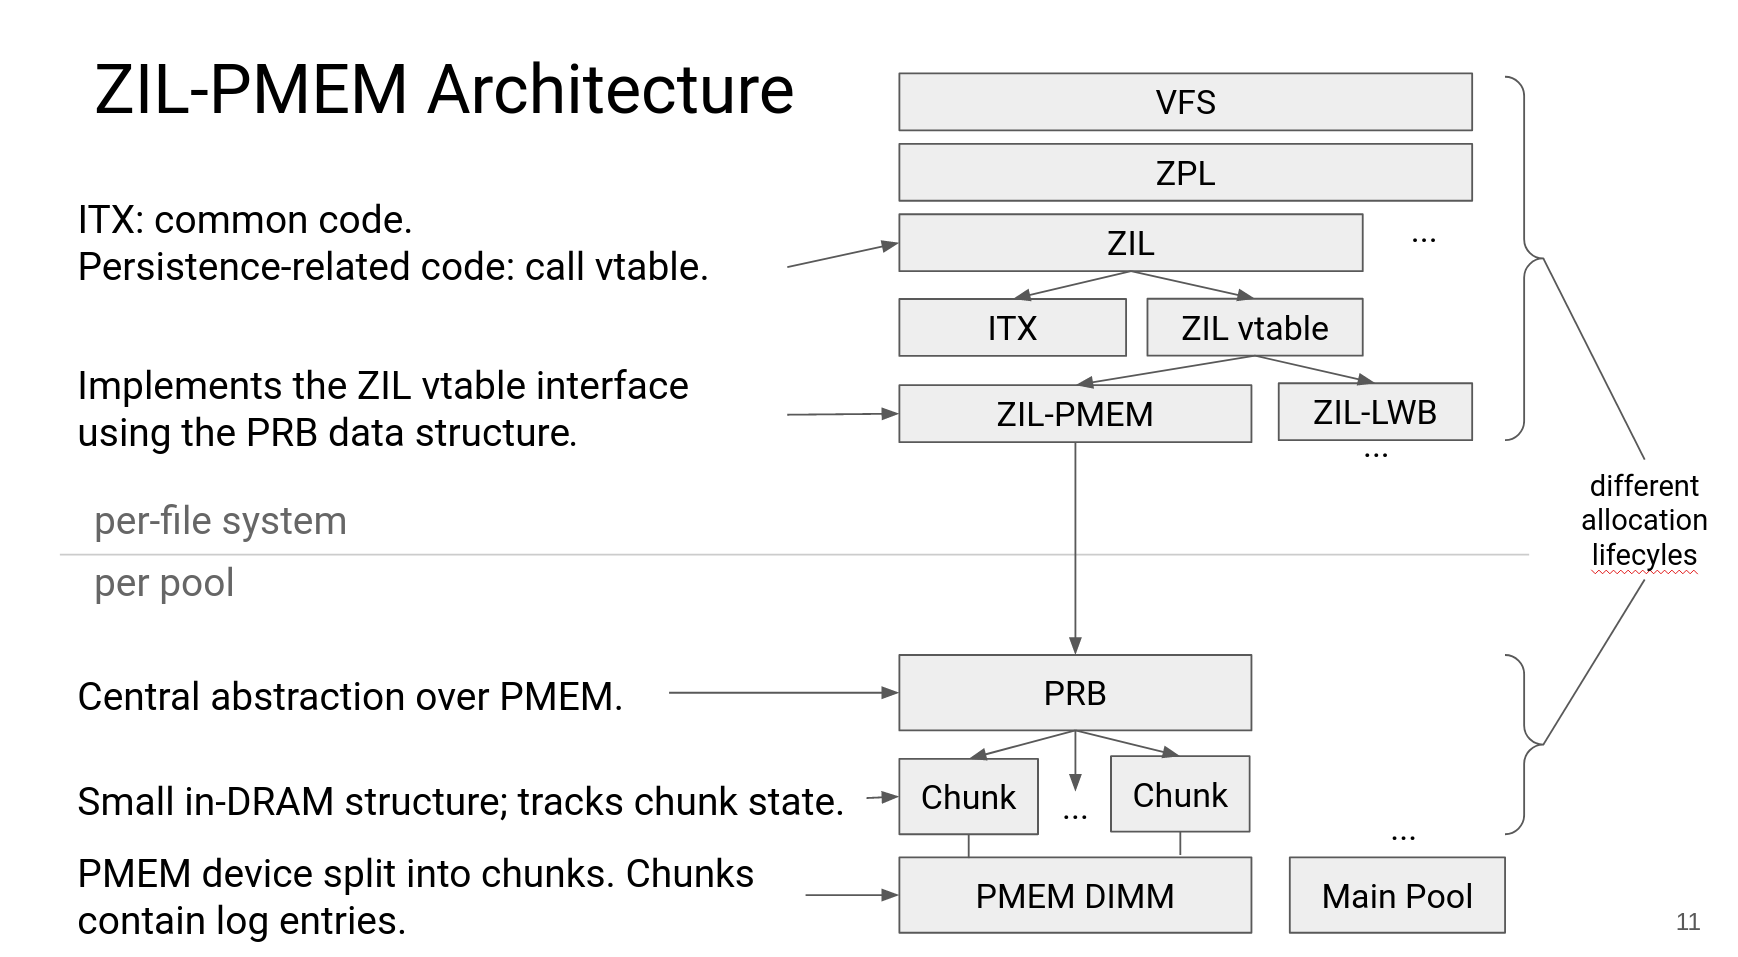
\includegraphics[height=20cm,angle=270,width=\textwidth,keepaspectratio]{fig/zilpmem_architecture_overview}
    \caption{Overview of the system architecture as described in this section.}
\end{figure}~\todo{actual figure}

\chapter{The PRB/HDL Data Structure}\label{ch:prbhdl}

In this chapter we describe the PRB/HDL data structure which implements the bulk of ZIL-PMEM's functionality\todo{language, help}.
PRB/HDL abstracts the allocatable space of a PMEM SLOG vdev into virtual logs for each dataset in the pool.
The \textit{zil\_pmem.c} module, which we present in Chapter~\ref{ch:zilpmem} uses these virtual logs to implement the ZIL-PMEM ZIL kind.
%A single PRB instance supports multiple logs with independent lifecycles.
%Each log is represented by a HDL object that provides methods for writing and replaying log entries.
%Log entries are opaque to PRB --- the only ZFS-specific metadata is the transaction group (txg) in which the log entry's effect will be synced.
%Knowledge of the entry's txg is necessary for log replay and log entry garbage collection.
%The \textit{zil\_pmem.c} module, which we present in Section~\ref{ch:zilpmem}, acts as a mere integration layer between the remainder of ZFS and PRB.
We present the design and implementation of PRB in a top-down manner.
In Section~\ref{di:prb:background} we recapitulate the role of the ZIL in ZFS to subsequently analyze the requirements that ZIL-PMEM puts on PRB in Section~\ref{di:prb:analysis}.
Afterwards, in Section~\ref{di:prb:approach}, we give a high-level overview of our design.
Section~\ref{di:prb:logstructure} presents the virtual log abstraction that is exposed by HDL and Section \ref{di:prb:replayapproach} describes the high-level approach for replay.
Sections \ref{di:prb:deptrack}, \ref{di:prb:modeldatacorruption}, and \ref{di:prb:ccrecovery} then progressively refine our understanding of replay and explain how data corruption and crash-consistency is addressed by HDL.
Subsequently, we describe PRB which is the storage substrate that the HDLs use for persistence:
Sections~\ref{di:prb:dramdatastructure} and \ref{di:prb:pmemdatastructure} present the data structures that we use for PMEM space management and log entry storage.
In Section~\ref{di:prb:traversal} we describe the algorithm that traverses the in-PMEM data structure during log recovery.
Secton~\ref{di:prb:gc} then explains how garbage collection removes entries from it\todo{help, don't want to repeat 'in-PMEM structure'}.
The low-latency and CPU efficient design of the write path is then presented in Section~\ref{di:prb:write}.
Finally, Section~\ref{di:prb:api} provides an overview of the PRB/HDL API that is consumed by \textit{zil\_pmem.c}.

\section{OpenZFS Background} \label{di:prb:background}
Remember from Section~\ref{openzfs:pool_operation} that whenever a file system call changes a dataset $D$, it does so in a DMU transaction $T_i$ within a transaction group $T_{i_{txg}}$.
After the system call handler has finished the DMU transaction by calling \lstinline{dmu_tx_commit(T_i)}, the logical change $C_i$ made in $T_i$ is not yet persisted to stable storage.
Instead, the DMU accumulates the changes from many DMU transactions in DRAM as so-called \textit{dirty state}, grouped by the transaction's txg.
Eventually, the \textit{txg sync} background thread syncs out a new version of the zpool state that contains the accumulated changes of the txg:
it first \textit{quiesces} the currently \textit{open txg} by not admitting new DMU transactions to it and waits for existing DMU transactions to finish.
Once all DMU transactions have finished, it is guaranteeed that the accumulated dirty state for this txg is not going not change.
The txg transitions to the \textit{syncing} state and txg sync starts to write out an updated version of the on-disk state.
After this process is complete, the transaction group is the pool's new \textit{last synced} txg.
Note that there are three unsynced txgs at any given time, one for each of the three states \textit{open}, \textit{quiescing}, and \textit{syncing}.
This improves DMU transaction latency because it decouples new DMU transactions from the \textit{txg sync} thread:
new DMU transactions can always operate on the open txg while txg sync only operates on the syncing txg.

The ZIL bridges the gap between the time at which a DMU transaction $T_i$ is finished (\lstinline{dmu_tx_commit}) and the time at which the changes made by $T_i$ actually reach the main pool through \textit{txg sync}.
For that purpose, the system call handler encodes the change $C_i$ that was made in $T_i$ as a \textit{log record}, wraps it in an \textit{ITX} and \textit{assigns} it to the ZIL.
The ZIL stores assigned ITXs in DRAM in the \textit{itxg} data structure.
If the system call has synchronous semantics, the system call handler invokes \lstinline{zil_commit} before returning to userspace.
\lstinline{zil_commit} uses \lstinline{itxg} to determine the \textit{commit list} which contains the sequence of ITXs that needs to be concatenated to some form of persistent log structure.
In upstream ZFS, the ZIL(-LWB) implements this persistent log structure by stuffing ITXs into LWBs and linking the LWBs into a chain on disk.
With the introduction of ZIL kinds, \lstinline{zil_commit} only builds the commit list and leaves the persistence to the ZIL kind implementation.

After a system crash, the zpool is in the state of the last synced transaction group which we call $precrash\_txg$.
Our dataset $D$ is lacking exactly those changes $C_i$ whose transactions $T_i$ were made in transaction groups that are younger than $precrash\_txg$, i.e., their $T_{i_{txg}} > precrash\_txg$.
When $D$ is mounted, these changes $C_i$ need to be applied to $D$ in order to recover data that was reported as committed towards userspace.
The ZIL API for this task is called \lstinline{zil_replay}.
Its implementation is specific to each ZIL kind but the API contract is the same:
the caller provides a callback that the implementation invokes for every log record that represents a missing change $C_i$.
The callback interprets the log record and performs a DMU transaction that atomically applies the change to the dataset and records replay progress in the ZIL header.
The invocation order is defined by \lstinline{itxg} through the commit list order at write time, but entries for transactions in txgs $T_{i_{txg}} \le precrash\_txg$ must be skipped because the change encoded in them is already part of the dataset state.
We provide an example for the commit list and the replay sequence for different precrash-txgs in Figure~\ref{fig:zil_writepath_and_replay_sequence_logical_level}.

\begin{figure}[H]
    \centering
    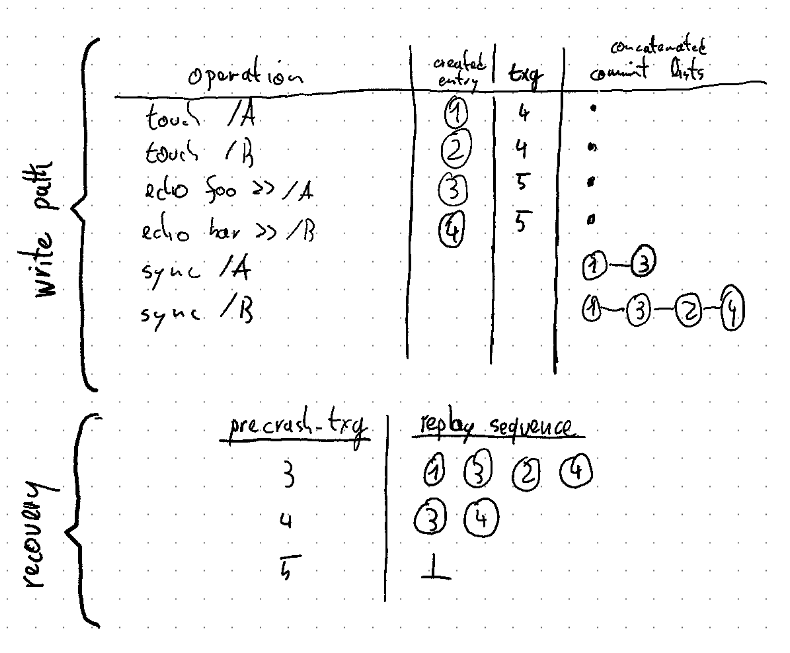
\includegraphics[height=6.5cm]{fig/zil_writepath_and_replay_sequence_logical_level}
    \caption{
        Example for a commit list with entries from different files and txgs.
        We show the replay sequences for different precrash-txgs.
        The replay callback must only be invoked for the entries that log changes in txgs younger than the precrash-txg.
    }
    \label{fig:zil_writepath_and_replay_sequence_logical_level}
\end{figure}

Note that the DMU transactions during replay only re-enact the logical changes to the dataset but do not restore the exact physical state of the dataset that would have been synced in the absence of a crash.
For example, changes that would have been spread across transaction groups 23, 24, and 25 at write time may land in transaction groups 42 and 43 during replay.
Further, the system could crash again, during replay.
For example, we could lose power so that txg 42 is the last-synced txg whereas 43 was still in \textit{syncing} state.
Since the replay callbacks for the individual log records are not idempotent, the ZIL must ensure that, after the crash during replay, the changes that were already replayed in transaction group 42 are not replayed again.
For example, the second replay attempt could apply the remaining set of changes in transaction group 83, but it may also be possible that they are spread over several txgs, e.g., 83 and 84.
The consequence for any ZIL implementation is that it needs to persist the following data, e.g., in the ZIL header:
\begin{description}[noitemsep,leftmargin=1.5cm,labelindent=1cm]
    \item[Precrash-txg] The \textit{precrash-txg} for open logs at the first time during pool import so that it can filter log entries by that criterion, and
    \item[Replay progress] Information that tracks which log entries have already been replayed so that replay can be resumed correctly after a crash.
\end{description}

\section{Requirements}\label{di:prb:analysis}

The \textit{commit list} is the point at which the common ZIL code hands over responsibility to the ZIL kind implementation.
We identify the following requirements for the persistence layer of any ZIL kind:
\begin{itemize}[noitemsep,beginpenalty=100000,midpenalty=100000]
\item During normal operation, it acts as a write-only sink for ITXs whose order is defined by the \lstinline{itxg} data structure in the form of the \textit{commit lists}.
\item The persistent representation of an ITX is the \textit{log record}.
    A log record is the encoded representation of the change that was made in a single DMU transaction.
    Log records are always scoped to a single dataset.
    Their representation is shared among all ZIL kinds.
    However, the ZIL kind introduces additional structures to encode the commit list order.
    For example, ZIL-LWB introduces the log-write Block (LWB) as explained in Section~\ref{ch:lwb_analysis:openzfs_background_zil_lwb}.
    ZIL-PMEM wraps log records in so-called \textit{log entries} that contain additional metadata.
\item In the event of a crash, the persistence layer must replay exactly those log records that have been successfully written to the ZIL but whose DMU transaction's txg did not sync before the crash.
    The code that decodes the log records and applies the changes encoded in them is shared among all ZIL kinds.
    It applies each log record's change in separate DMU transactions and gives the persistence layer an opportunity to update the ZIL header in the same transaction.
\item Each dataset has a separate log that is written and replayed independently.
\end{itemize}
We derive the following abstract view of \textbf{what} needs to be stored \textbf{per log}:
\begin{itemize}[noitemsep,beginpenalty=100000,midpenalty=100000]
    \item The log records themselves.
    \item The transaction group of the DMU transaction that the log record encodes.
    \item Structural information that defines replay order and/or logical dependencies between log entries that replay must respect.
    \item The \textit{precrash-txg} to discern replayable from obsolete log records (see previous section).
    \item Some representation of \textit{replay progress} to enable resumption of replay if the system crashes during replay.
\end{itemize}
For ZIL-PMEM, we put the following requirements on the \textbf{storage substrate} that stores the log entries:
\begin{itemize}[noitemsep,beginpenalty=100000,midpenalty=100000]
    \item On the write path, the overhead added to the raw log entry write time should be minimal.
    \item It must scale well on a multicore system since many datasets write their log entries in parallel.
        This scalability requirement includes efficient use of CPU time in case the PMEM write bandwidth is exceeded.
    \item The storage substrate is responsible for garbage-collecting log entries after they are obsolete, either by txg sync during normal operation or because they have been replayed.
    \item It must provide a facility to retrieve non-obsolete log entries of a dataset for replay.
    \item It must detect data corruption using checksums. (Repair and redundancy are out of scope for this thesis, see Section~\ref{sec:requirements}.)
\end{itemize}

\section{Approach}\label{di:prb:approach}
We introduce the pool-wide \textit{PRB} object which abstracts the PMEM SLOG vdev's space as a persistent, unordered set of log entries.
A log entry encodes a logical change to a particular dataset that was applied in a single DMU transaction.
PRB provides facilities for adding log entries to the set and for iterating over its contents.
It automatically garbage-collects entries after they become obsolete because their transaction group has synced.

Log entries are created by the thread that performs the DMU transaction.
However, the thread does not write them directly to PRB but to the \textit{HDL} object of the modified dataset.
A HDL is a virtual log built on top of PRB that organizes individual entries for a single dataset in a mostly sequential structure.
After a system crash, the HDL provides a replay facility that recovers the replayable entries, orders them according to their logical dependencies, and handles missing entries.

At any time, there exists one HDL for each head dataset in the pool.
They are set up early during pool import and torn down late during export.
If a dataset is created or destroyed, the corresponding HDL is set up or torn down as well.
HDL is stateful.
Its internal states represent the different phases that a dataset goes through with regards to the ZIL.

\begin{figure}[H]
    \centering
    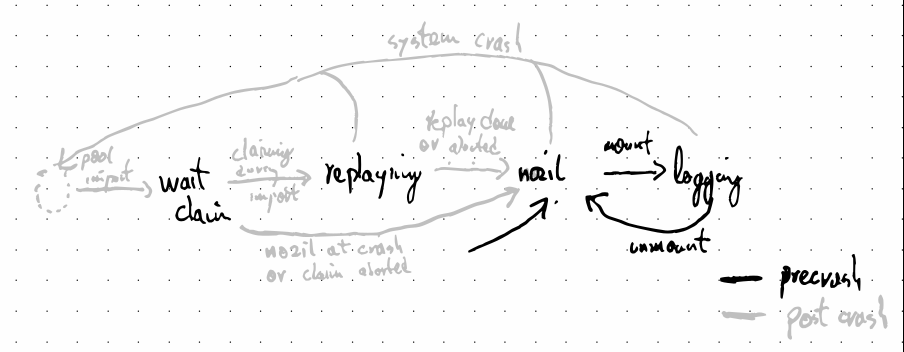
\includegraphics[height=5cm]{fig/prb_hdl_runtime_states}
    \caption{TODO}
\end{figure}

When the HDL is created, it does not have a log and is in state \textit{nozil}.
When the dataset is mounted, the HDL allocates a log GUID which uniquely identifies the log's entries in the PRB and persists it to the ZIL header.
The HDL is now in state \textit{logging} and threads can write entries to it.
If the dataset is unmounted, the log GUID is discarded and the log transitions back to state \textit{nozil}.
Otherwise, the HDL remains in state \textit{logging} until the system crashes.

When a zpool is imported, the \textit{claiming} phase examines the ZIL header of each dataset to recover the HDL's runtime state from before the crash.
If the HDL state was \textit{logging}, the claiming procedure saves the zpool's \textit{last synced} txg as the \textit{precrash-txg} and transitions the HDL and ZIL header to state \textit{replaying} in initial replay position.
If the HDL was already in state \textit{replaying}, the precrash-txg and replay position are recovered from the ZIL header.
At this point, all HDLs are either in state \textit{nozil} or \textit{replaying}.
HDLs in state \textit{replaying} scan the PRB for log entries that need to be held back for replay.
Entries that are held back by at least one HDL are exempt from PRB's garbage collection.
After this step, the claiming phase is done and the txg sync thread starts.
HDLs are not replayed until their dataset is mounted which happens on a per-dataset basis at a user-controlled point in time. %which can be deferred indefinitely by the user, might not happen for several zpool import/export cycles, or system crashes.
After replay is complete, the HDL discards the log GUID and transitions to state \textit{nozil}.
At this point, the mount procedure behaves as if log replay had not happened and starts a new log with a new log GUID, thereby closing the circle.
Note that the HDL (and PRB) are able to tolerate a system crash in any of the HDL or ZIL header states.
We address this issue in Section~\ref{di:prb:ccrecovery}.

\section{HDL: Log Structure}\label{di:prb:logstructure}
The structure of the virtual log that each HDL represents is defined by metadata stored with each entry that is written to PRB.

We \textbf{attribute} entries to a given HDL's log through the \textit{log GUID}:
\begin{description}[noitemsep,leftmargin=1.5cm,labelindent=1cm]
    \item[Log GUID] A 128 bit random identifier stored in the HDL's ZIL header and repeated in every entry written through that HDL.
\end{description}

The following pieces of metadata define the structure of the log.
\begin{description}[noitemsep,leftmargin=1.5cm,labelindent=1cm]
    \item[Transaction Group (txg)] The transaction group in which the change encoded in the entry was or would have been synced out by \textit{txg sync}.
    \item[Generation Number (gen)] The log is a sequence of generations, each of which contains many log entries.
        The generations encode logical dependencies between entries.
        Entries within the same generation do not depend on each other.
        Entries from newer generations unconditionally depend on all entries in all previous generations.
        We represent generations as unsigned 64-bit non-zero integers.
    \item[Generation-Scoped ID (gsid)] Within a generation, we identify entries by another by the $gsid$, another unique unsigned 64-bit non-zero integer.
        As the name suggests, the $gsid$ only needs to be unique within a generation.
\end{description}
Note that the tuple $(gen, gsid)$ unqiuely identifies an entry within a log.

We visualize the structure of the log in a grid.
The rows represent the transaction group ($txg$) and the columns represent the generation ($gen$).
For readability, we represent entries not by $(gen, gsid)$ but by a single unique letter.
The projection of entries onto the horizontal axis shows the dependency relationship encoded by the generations.
The projection of entries onto the vertical axis shows the sets in which entries are garbage-collected.

\begin{figure}[H]
    \centering
    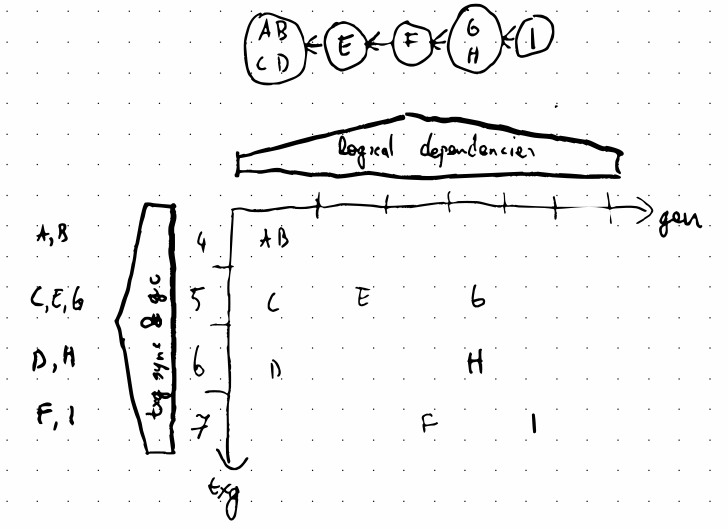
\includegraphics[height=8cm]{fig/prb_hdl_log_structure_example}
    \caption{Structure of a single HDL's log as described in the previous paragraph.}
    \label{fig:prb_hdl_log_structure_example}
\end{figure}

\section{HDL Replay: Basic Approach}\label{di:prb:replayapproach}
Replay must apply the changes that were successfully logged to the HDL but whose DMU transaction did not sync before the system crashed.
To accomplish this task, it scans the PRB for entries that belong to the HDL and determines a \textit{replay sequence} $S$.
\begin{align*}
    & \text{Entry}~E_i \in S \\
    \Leftrightarrow & E_i.log\_guid = HDL.log\_guid \wedge E_i.txg > precrash\_txg
\end{align*}
$S$ is sorted in \textit{replay order}, which is the order the changes encoded in the entries need to be applied.
Given two entries $E_a$, $E_b \in S$ for the same HDL, the replay order is a total order defined by
\begin{align*}
    & E_a <_{replay} E_b \\
    \Leftrightarrow &  (E_a.gen, E_a.gsid) <_{lexicographical} (E_b.gen, E_b.gsid) \\
    \Leftrightarrow & E_a.gen < E_b.gen \vee (E_a.gen = E_b.gen \wedge E_a.gsid < E_b.gsid) \\
\end{align*}
For our example in Figure~\ref{fig:prb_hdl_log_structure_example}, this results in the following replay sequences, depending on the value of $precrash\_txg$.

\begin{figure}[H]
    \centering
    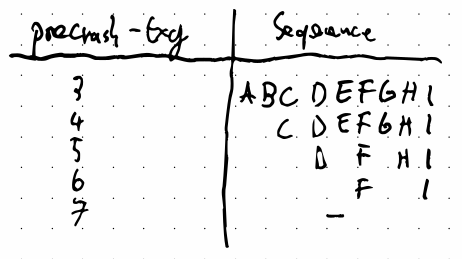
\includegraphics[height=4cm]{fig/prb_hdl_log_structure_example__replay}
    \caption{Replay sequences for the log depicted in Figure~\ref{fig:prb_hdl_log_structure_example}, by $precrash\_txg$. }
    \label{fig:prb_hdl_log_structure_example__replay}
\end{figure}

We use a total order so that we can precisely encode replay progress by storing the last-replayed $(E.gen, E.gsid)$.
This is necessary for crash consistency because log entry replay is not idempotent.
We revisit this topic in Section~\ref{di:prb:ccrecovery}.

Note that the definition of the replay order does not account for overflows of $gen$ or $gsid$ --- entries written after the overflow would be incorrectly ordered as smaller than entries written before the overflow.
Overflows could be handled in software, e.g., by temporarily destroying the log of the dataset and creating a new one with a fresh log GUID.
However, our implementation has no such provisions because even with the (absurdly) conservative of \SI{1}{ns} write time per log entry, the first overflow event would only occur in \SI{584}{years} if $gen$ starts at~$1$.

\section{HDL Replay: Dependency Tracking}\label{di:prb:deptrack}
% \begin{description}
    %     % \item[Garbage Collection] After a txg $t_{synced}$ has been synced, PRB garbage-collects all entries $\mathcal{E}_{gc} := { E : E.txg \le t_{synced}}$.
    %     %     This does not interfere with replay because, if the system crashes, it is guaranteed that $precrash\_txg \le t_{synced}$ and hence $\mathcal{e}_{gc}$ would never be part of a replay sequence.
    %     \item[Loss of Entries] If such a missing entry $E_m$ with $E_m.txg > precrash\_txg$ is missing, any entry $E_d$ that logically depends on $E_m$ ($E_m < E_d$) and is for an unsynced txg ($E_d.txg > precrash\_txg$) must no longer be replayed.
        % However, all entries $E_p$ that do not depend on $E_m$ ($E_p \le E_m$) and need replay ($E_p.txg > precrash\_txg$) should still be replayed.
    % \end{description}
Replay is complicated by the fact the entries that were stored in the PRB can be lost.
For example, bitflips in PMEM might corrupt the entry's log GUID or PRB-internal metadata.
If an entry $E_m$ with $E_m.txg > precrash\_txg$ is missing, any entry $E_d$ that logically depends on $E_m$ ($E_m < E_d$) and is for an unsynced txg ($E_d.txg > precrash\_txg$) must no longer be replayed.
However, all entries $E_p$ that do not depend on $E_m$ ($E_p \le E_m$) and need replay ($E_p.txg > precrash\_txg$) should still be replayed.

We detect missing entries through a set of counters that we store in the metadata of each entry.
For an entry $E$, the counter $E.C_{ctxg_i}$
\begin{gather*}
    E.C_{ctxg_i} := \#\{ D : D.gen < E.gen \wedge D.txg = ctxg\_i\}
\end{gather*}
stores the number of entries that were written to the log since its inception, for a DMU transction with txg $ctxg\_i$, until generation $E.gen$.
During replay, we first construct the replay sequence (example in the previous section, Figure~\ref{fig:prb_hdl_log_structure_example__replay}).
Then, we re-compute and compare the counters for each entry in the replay sequence.
If an entry $E_m$ has been lost, the counters of any dependent entry $E_d$ (their $E_d.gen > E_m.gen$) will not match, causing replay to stop with $E_d$ as a \textit{witness}.
Missing entries in the last generation (the ``tail'' of the log) cannot be detected with this scheme.

The per-txg scoping of the counters is critical to accomodate garbage collection.
Suppose we only used a single sequence counter for all log entries of a HDL.
After a txg $t_{synced}$ has been synced, PRB garbage-collects all entries $\mathcal{S}_{gc}$ that are obsolete:
\begin{align*}
    \mathcal{S}_{gc} := \{ E : E.txg \le t_{synced}\}
\end{align*}
These entries no longer show up when the claiming or replay procedures scan the PRB for entries with the HDL's log GUID.
If we used a single sequence counter to check for missing entries, we would be unable to discern garbage-collected entries from missing entries.

It is sufficient include only those counters $E.C_{txg_i}$ in the entry metadata whose transaction groups $txg_i$ had not yet been synced at the time that $E.gen$ started.
The reason is that a~) the replay sequence only contains entries in unsynced txgs and b~) $E$ only depends on entries $D$ with $D.gen < E.gen$.
Since there are only three possible unsynced txgs at any time (\textit{open}, \textit{quiescing}, \textit{syncing}), we only need to store three $(txg_i, C_{txg_i})$ tuples per log entry.
In fact, since txgs never skip a number, we only store the value of $txg_{open}$ and recompute
\begin{align*}
    txg_{quiescing} & = txg_{open} - 1 \\
    txg_{sycing} & = txg_{open} - 2
\end{align*}
\todo{compact encoding is just an idea, not in impl yet}

We use the same algorithm to compute the counters on both the write and recovery path.
This works because the write path must use monotonically increasing generation numbers, and the entries in the replay sequence are sorted in that order.
The counters are stored in a table called \textit{live table}.
It has four rows $R_i := (txg, ctr), i \in \{0,1,2,3\}$.
When an entry $E$ is written or visited, it modifies the counter in the row with index $I_T := T \mod 4$ where $T := E.txg$.
We distinguish the following conditions:
\begin{itemize}[noitemsep]
\item If $R_{I_T}.txg = T$, we simply increment $R_{I_T}.ctr$ and are done.
\item If $T > R_{I_T}.txg$, we can infer that txg $R_{I_T}.txg$ must have been synced out because there are only three unsynced txgs at any given time but four array entries that are reused in a circular manner, curtesy of indexing by $T\mod 4$.
In that case, we can discard the state in the row and reuse it for $T$ by setting $R_{I_T} \leftarrow (T, 1)$.
\item Conversely, if $T < R_{I_T}$, we can infer that the entry we are writing is for an already synced txg and hence obsolete.
In that case, we do not change the \textit{live table} and turn the entry write operation into a no-op.
\end{itemize}
Note that the use of 4-ary arrays allows the use of \textit{bitwise-and} for indexing, which is a common ZFS idiom (\lstinline{table[txg&3]}).

To detect the start of a new generation and support crash-consistent replay, we maintain a separate variable $E_{last} := (gen, gsid)$.
When an entry $E$ is written or visisted, we compare it to $E_{last}$ using the following rules:
\begin{description}[noitemsep,leftmargin=1.5cm,labelindent=1cm]
\item[$E < E_{last}$] This case is prohibited because the API contract for log writers is that generation numbers must be monotonically increasing.
We consider the log corrupted if such an entry $E$ is found.
\item[$E.gen = E_{last}.gen$] The writer did not start a new generation and we leave the \textit{last table} unmodified.
\item[$E.gen > E_{last}.gen$] We create a copy of the \textit{live table}. We refer to this snapshot as \textit{last table}.
\end{description}
Regardless of whether a new generation was started or not, we always update $E_{last} \leftarrow E$ and increment the counter in the \textit{live table} as described in the previous paragraph after evaluation the rules above.

The counters $E.C_{txg_i}$ have the same value for all entries in generation $E.gen$  because, by defintion, they only count entries written up to but not including $E.gen$.
Hence we compute them from the \textit{last table} once and cache the results until the next generation is started:
\begin{enumerate}[noitemsep]
    \item Determine row index $i_{max} := \max_{i \in \{0,1,2,3\}} R_i.txg$ where $R_i \in \text{last table}$.
    \item Invariant: $R_{i_{max}}.txg$ is the highest potentially unsynced txg in generations $< open\_gen$.
        We make the most conservative assumption that $R_{i_{max}}.txg$ was the \textit{open txg} in generation $open\_gen - 1$.
    \item Find the counters for \textit{quiescing} and \textit{syncing txg}.
        We scan the \textit{last table} twice to find counters for transaction groups $R_{i_{max}}.txg - 1$ and $R_{i_{max}}.txg - 2$.
        If the \textit{last table} does not contain those counters, we use a value of zero.
\end{enumerate}

Figure~\ref{fig:prb_counters_table__computation} contains a graphical illustration of the algorithm described above.
Figure~\ref{fig:prb_counters_table__encoding} shows how we encode the counters in the entry header.
We provide an extensive example in Figure~\ref{fig:prb_counters_table__example}.

\begin{figure}[H]
    \centering
    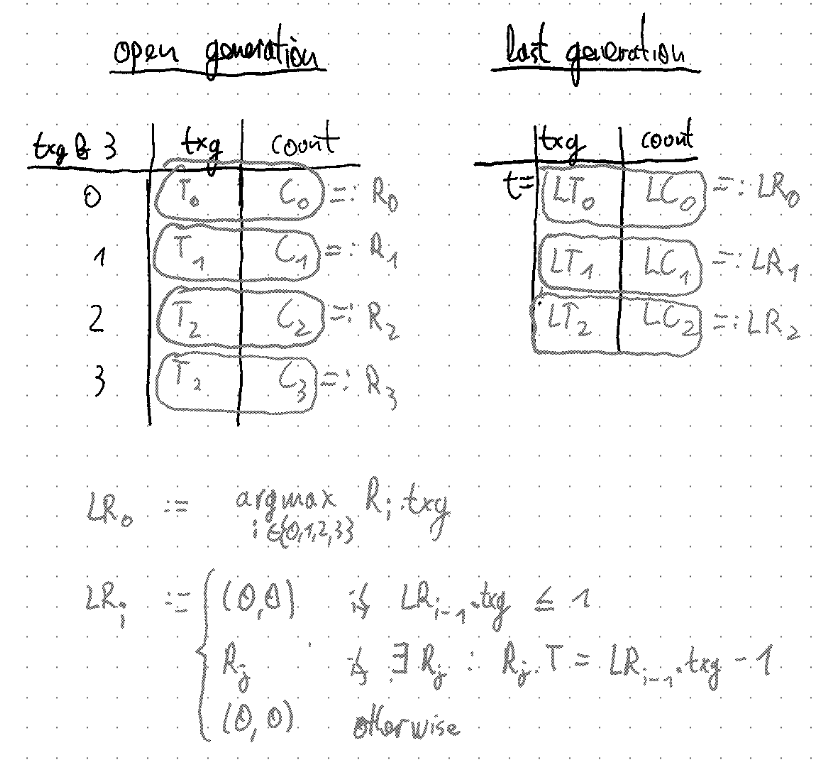
\includegraphics[height=10cm]{fig/prb_counters_table__computation}
    \caption{
        Visualization of the \textit{live} and \textit{last table} structures, and a declarative definition of how the \textit{last table} is computed.
        %Note that we also provide an Example in Figure~\ref{fig:prb_counters_table__example}.
    }
    \label{fig:prb_counters_table__computation}
\end{figure}

\begin{figure}[H]
    \centering
    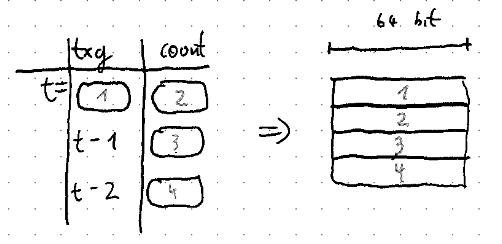
\includegraphics[height=4cm]{fig/prb_counters_table__encoding}
    \caption{Space-efficient encoding of the counters.}
    \label{fig:prb_counters_table__encoding}
\end{figure}

\begin{figure}[H]
    \centering
    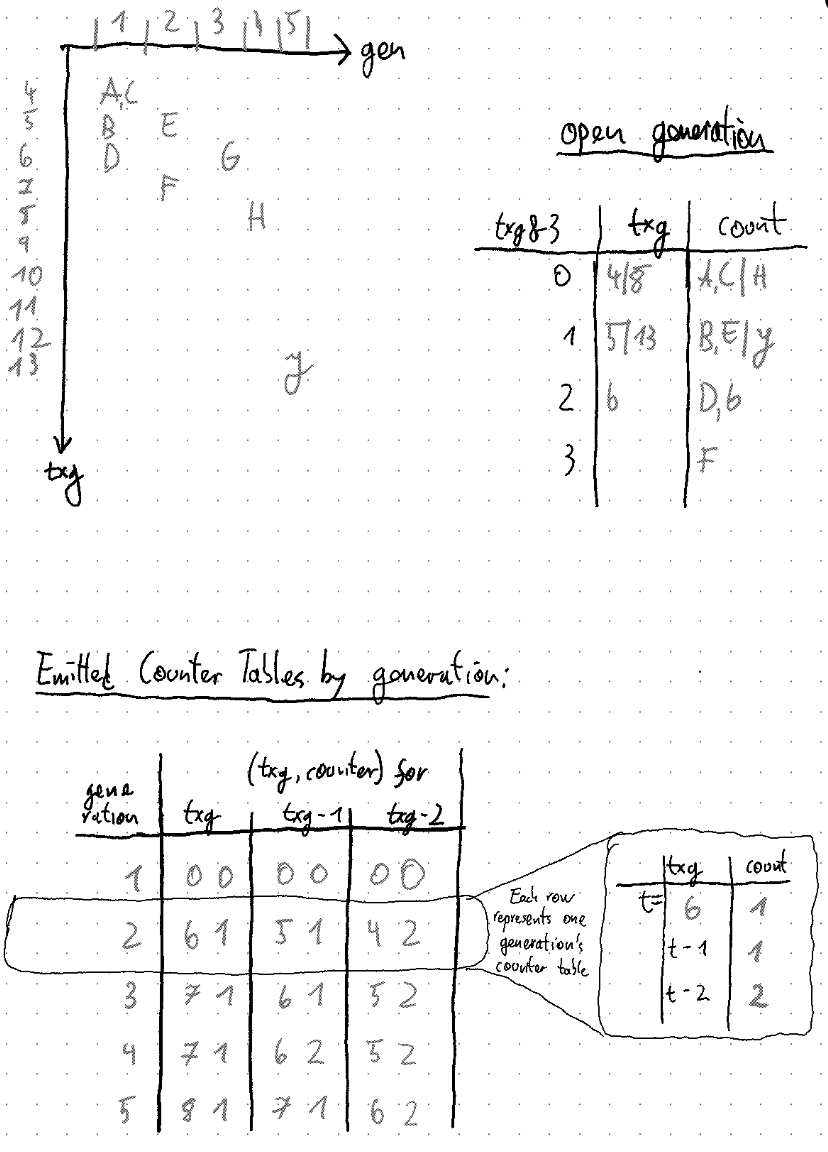
\includegraphics[height=16cm]{fig/prb_counters_table__example}
    \caption{
        Example for the computation of the counters that are stored in the entry.
        The following entries are written to the log:
        A,B,C,D in generation 1; E,F in generation 2; G in generation 3; H in generation 4; J in generation 5.
        Note that their txgs differ sometimes but stay in a corridor of at most three txgs.
        The table at the bottom shows the counter values in the entry headers:
        each row represents the counter table that is stored in the entry headers of one generation.
        The table at the upper right shows the algorithm's table's content over time.
        Instead of counters, we show the entries that would cause the specific counter to be incremented.
        We visualize row-reuse by separating new row content with a ``\lstinline{|}" symbol in each cell of the reused row.
    }
    \label{fig:prb_counters_table__example}
\end{figure}

\section{HDL: Model For Data Corruption}\label{di:prb:modeldatacorruption}
The use of counters to validate that no log entries are missing relies on the assumption that random data corruption is incapable of ``forging'' new log entries.
If this were possible, a forged entry could compensate a lost entry in the counter table.
The loss of the entry would go unnoticed and the replay of the forged entry would likely corrupt the dataset.

We believe that it is sufficiently unlikely for random data corruption to accidentally forge an entry.
A forged entry would have to fulfill the following requirements to affect counter validation for a given log $L$:
\begin{itemize}[noitemsep]
    \item It must have been correctly added to PRB's data structures such that a scan of PRB will find it during recovery.
        (We address the PRB's data structure in Section~\ref{di:prb:pmemdatastructure}.)
    \item Its \textit{log GUID} value must match log $L$'s log GUID.
    \item Its $(gen, gsid)$ must not collide with the original entries.
        Such a collision would be noticed when constructing the replay sequence.
        (Our implementation uses a b-tree that identifies and sorts nodes by $(gen, gsid)$).
    \item Its \textit{txg} value must be in the correct corridor of unsynced txgs and generation.
        If the txg is too old or too young, the forged entry would be noticed by the dependency tracking code when re-computing the counters (see previous section).
\end{itemize}

Apart from random data corruption, we have considered the following scenarios and concluded that they are out of scope for ZIL-PMEM:
\begin{itemize}[noitemsep]
\item Implementation errors on the write path.
\item Firmware bugs, e.g., in the Optane DIMM's wear-leveling layers, that could make old entries re-appear.
\item Deliberate injection of log entries by a malicious party with write access to PMEM.
    This needs to be part of the threat model if ZIL-PMEM is extended to support OpenZFS Native Encryption.
    Forged entries should be trivially detectable by cryptographically authenticating the entry header, e.g. using the AEAD ciphers that are already in use for the encryption feature.
\item Accidental reuse of \textit{log GUIDs}.
    If two HDLs use the same log GUID to write their entries, the HDLs will each claim their and the other HDL's entries.
    This scenario is very unlikely because we generate log GUIDs as 128 bit random numbers and check for collisions with other HDLs.
\end{itemize}

\section{HDL: Replay Crash-Consistency}\label{di:prb:ccrecovery}

The PRB and its HDLs must be able to tolerate a system crash at any time in their lifecycle.
With regards to recovery, this means that claiming must be restartable and replay resumable across crashes.
Further, the restarted or resumed recovery procedure must be able to handle online and offline loss of entries due to data corruption.

Crash-consistency for claiming is trivial because it runs during pool import before txg sync starts.
Thus, all changes made by claiming are accumulated in DRAM and atomically persisted by the first transaction group that is synced after pool import.
From the perspective of HDLs that are in state \textit{logging}, this first transaction group is $precrash\_txg + 1$.
If the system crashes before that txg is synced, a subsequent import attempt restarts from the same state as the previous one.
HDLs that are already in state \textit{replaying} make no modifications during claiming --- they only build up DRAM state, i.e., the set of entries held back for replay.

Replay is complicated by two additional aspects:
\begin{itemize}[noitemsep]
    \item Replay of an individual log entry is not idempotent.
    \item Replay is spread across several transaction groups and hence not atomic.
        (See this chapter's Section~\ref{di:prb:background} on OpenZFS background.)
\end{itemize}
Our solution is to externalize all state of the replay algorithm, including the counters used for dependency tracking, to a structure called \textit{replay state}.
Whenever we replay an entry, we checkpoint \textit{replay state}.
We store the latest checkpoint in the ZIL header every time we replay an entry.
If the system crashes, we recover \textit{replay state} from the checkpoint in the ZIL header.

The following variables are stored in \textit{replay state}:
\begin{description}[noitemsep,leftmargin=1.5cm,labelindent=1cm]
    \item[$\mathbf{(gen_{last}, gsid_{last})}$] The $(E.gen, E.gsid)$ of the last entry $E$ that was replayed.
    \item[Live Table] The \textit{live table} at the time the entry was replayed, i.e., $R_i$ with $i~\in~{0,1,2,3}$.
    \item[Last Table] The \textit{last table} at the time the entry was replayed.
    \item[$E_{seal}$] An artificial entry header that is used to detect lost entries at the end of the log structure.
\end{description}
The crash-safe replay procedure performs the following steps:
\begin{enumerate}[noitemsep,beginpenalty=100000,midpenalty=100000]
    \item \label{ccReplay:claimscan} Claiming reads the log GUID from the ZIL header, then scans the PRB and holds back the log's entries from garbage collection.
    \begin{itemize}[noitemsep,beginpenalty=100000,midpenalty=100000]
        \item \label{ccReplay:transitionToReplaying} If the HDL is in state \textit{logging}, claiming transitions the ZIL header to \textit{replaying} and initializes the \textit{replay state} checkpoint in the ZIL header.
            \begin{itemize}
                \item $(gen_{last}, gsid_{last})$ is $(0, 0)$.
                \item \textit{live table} and \textit{last table} are zeroed out.
                \item $E_{seal}$ is determined as follows.
                \begin{enumerate}
                    \item Construct a temporary replay sequence $S_{tmp} = \{E_s : s \in 1, \dots, n\}$.
                    \item In DRAM, append an artificial entry $E_{n+1}$ to $S_{tmp}$.
                        $E_{n+1}.gen = E_{n}.gen + 1$, $E_{n+1}.gsid = 1$, and $E_{n+1}.txg = E_{n}.txg$.
                    \item Iterate over $S_{tmp}$ and compute the counter tables.
                        Validate the tables for $E_{1,\dots,n}$.
                        When arriving at $E_{n+1}$, assign the expected table to $E_{seal}$.
                \end{enumerate}
            \end{itemize}
        \item If the HDL is already in state \textit{replaying}, the ZIL header is not modified.
    \end{itemize}
    \item Replay recovers its \textit{replay state} from the checkpoint $C$ in the ZIL header.
    \item \label{ccReplay:construct_sequence} Replay constructs a replay sequence $S$ from the held back entries.
    \item While replaying $S$, the following happens for each entry $E_s \in S$:
        \begin{enumerate}[noitemsep,beginpenalty=100000,midpenalty=100000]
            \item \label{ccReplay:skipreplayed} Skip $E_s$ if it has already been replayed, i.e., $(E_s.gen, E_s.gsid) \le (C.E_{last}.gen, C.E_{last}.gsid)$.
            Otherwise:
            \item Create a backup checkpoint $C_b$ of \textit{replay state}.
            \item Perform dependency tracking as described in the previous section.
            \item Create a checkpoint $C_{E_s}$.
            \item In one DMU transaction, replay $E_s$ and store $C_{E_s}$ in the ZIL header.
            \item If replay fails or the DMU transaction fails, abort the transaction and roll back the in-DRAM version of \textit{replay state} to $C_b$.
    \end{enumerate}
\end{enumerate}

Note that steps~\ref{ccReplay:claimscan}~and~\ref{ccReplay:construct_sequence} construct a \textit{new} replay sequence every pool import.
This allows handling of offline data corruption in PRB.
Assume that we lose an entry $E_m$ while the system is offline.
If $E_m.txg \le precrash\_txg$, the loss of the entry is unnoticed because $E_m$ is by definition not part of the replay sequence.
If $E_m$ is skipped by step~\ref{ccReplay:skipreplayed}, the loss of the entry might be worth reporting but does not affect replay because it has already been replayed.
Otherwise, dependency tracking will eventually detect that $E_m$ is missing if, and only if, any other entry depends on it.
$E_{seal}$ is an artificial dependency to ensure that lost entries in the last generation are be detected.
\todo{this is not yet implemented}

We handle online data corruption as follows.
Claiming and replay only operate on DRAM-buffered copies of the entry metadata called \textit{replay node}.
When replaying an entry, the replay callback is forced to use a special function that attempts to read the entry from PRB and buffers it in DRAM.
Before allowing access to the entry, it ensures that the entry metadata still matches the data in the \textit{replay node}.
If either the read from PRB fails (e.g., due to checksum errors) or if the metadata does not match, we know that the entry has been corrupted since the PRB scan.

Note that the last generation $E_{seal}.gen - 1$ of the log structure is not protected against re-appearing log entries.
Assume that during initial claiming, entries $(42,1)$ and $(42,3)$ in generation $42$ are observed as the last entries of the replay sequence.
Then $(E_{seal}.gen, E_{seal.gsid)}$ is $(43,1)$ and the counter table of $E_{seal}$ only accounts for these two entries, and all previous generation's entries.
Now assume that another entry $(42,2)$ had been written but was temporarily invisible during initial claiming, e.g., due to temporary data corruption.
If for some reason $(42,2)$ becomes visible again, and we start replaying, then $(42,2)$ will be replayed even though it was not visible during claiming.
And if $(42,2)$ were to replace $(42,1)$ or $(42,3)$, we would not even notice the counter mismatch when arriving at $E_{seal}$.
This behavior seems desirable in the sense that replay recovers as much committed data as possible.
However, in combination with WR\_INDIRECT ZIL log records, it can lead to pool corruption.
ZIL-PMEM does not currently support WR\_INDIRECT records due to this problem as well as another WR\_INDIRECT-related issue that affects ZIL-LWB.\todo{link github issue on leaking allocated blocks}
Our proposed solution in the OpenZFS issue tracker could be used by ZIL-PMEM to properly detect changes to the last generation after claiming, and to support WR\_INDIRECT if desired.

\section{PRB: DRAM Data Structure}\label{di:prb:dramdatastructure}
The central requirements for PRB are
\begin{itemize}[noitemsep]
    \item persistence of log entries in PMEM,
    \item parallel insertion of log entries from multiple threads and HDLs,
    \item garbage collection of obsolete log entries,
    \item measures to detect data corruption.
\end{itemize}

Our design is built around the \textit{chunk} abstraction.
A chunk is a contiguous segment of PMEM that acts as an insert-only container for log entries.
PRB's role is to mediate access between HDLs and chunks.
When a thread writes an entry to the conceptual \textit{set of entries} that is the PRB, it actually inserts the entry into one of the PRB's chunks.
Once a chunk is full, PRB lets it sit unmodified until all entries in it are obsolete.
Garbage collection then removes all entries in those obsolete-only chunks and makes them available for reuse by writers.
The PRB scanning done by claiming and replay is implemented as an iteration over the entries in all chunks of the PRB.
If a chunk contains at least one candidate entry for replay, the claming HDL holds the chunk back from the write path and/or garbage collection.
Note that this design fully decouples storage location (chunk) from log structure (encoded in entry metadata, see previous sections).

Each chunk is represented by a DRAM object that holds the following values:
\begin{description}[noitemsep]
    \item[PMEM location] The chunk's start and end address in PMEM. These values do not change for the lifetime of the chunk.
    \item[Claim refcount] The number of HDLs that claimed at least one entry in the chunk for replay.
        Chunks with non-zero claim refcount are exempt from garbage collection and the write path.
    \item[Max txg] The maximum transaction group of the entries that were written to this chunk.
        This value is used by garbage collection to determine when all entries in the chunk are obsolete.
    \item[Write position] The PMEM address where the next entry will be written.
        We dicsuss the PMEM layout of the chunk in more detail in Section~\ref{todo}.
\end{description}

We move chunks between the following data structures to keep track of their current role within PRB.
\begin{description}[noitemsep]
    \item[Commit Slots]
    PRB maintains a roster of \textit{commit slots}, each of which has an associated \textit{open chunk}.
    When a thread writes an entry through a HDL, the thread first \textit{acquires} a commit slot to gain temporary exclusive access to its \textit{open chunk}.
    Then, it writes the entry to the open chunk and immediately releases the slot so that other threads can aquire it.
    \item[Free List]
    The \textit{free list} holds empty chunks.
    Their \textit{claim refcount} and \textit{max txg} is zero and their write position is reset to the chunk's start address.
    A log writer that needs a new chunk for its commit slot puts the commit slot's current open chunk on the \textit{full list} (see below) and gets a new chunk from the \textit{free list}.
    \item[Full Lists]
    The \textit{full lists} contains chunks that wait for garbage collection.
    PRB maintains one full list for each unsynced txg $T_i$. The \textit{full list} for $T_i$ contains exactly those (full) chunks whose \textit{max txg} is $T_i$.
    After $T_i$ has been synced, the chunks on the corresponding \textit{full list} are emptied and moved to the \textit{free list}.
    Note that it is sufficient to maintain three full lists at any given time --- one for each of the three unsynced transaction groups \textit{open}, \textit{quiescing}, and \textit{syncing}.
    The three lists can be represented as an array of three lists that is indexed by $T_i \mod 3$.
    Our implementation follows the common ZFS idiom of using four lists that are indexed by \lstinline{T_i&3} where \lstinline{&} is the \textit{bitwise and} operation.
    \item[Wait Replay List]
    During the claiming phase, all of the PRB's chunks are on the \textit{wait replay list}.
    The HDL's scan the chunks on this list during claiming.
    If a chunk contains at least one entry that needs to be held back for replay, the HDL increments the chunk's \textit{claim refcount}.
    Once claiming is done and \textit{txg sync} triggers the first garbage collection cycle, any chunk on this list that has a zero refcount is emptied and moved to the \textit{free list}.
    The list is also scanned for zero refcounts during all future garbage collection cycles to garbage-collect chunks that are no longer held by HDLs because they finished replay.
    Note that it is critical for replay crash consistency to defer garbage collection until \textit{after} the last txg of replay of the last HDL that held the chunk has synced.
    If we garbage-collected entries before the last holding HDL's ZIL header has transitioned to state \textit{nozil} on disk and crashed inbetween, the garbage-collected entries might be missing when resuming replay.
\end{description}

Figure~\ref{fig:prb_chunk_ownership_cycle__transitions} visualizes transitions of the chunks over their lifetime.
Figure~\ref{fig:prb_chunk_ownership_cycle__example} provides a corresponding example.

\begin{figure}[H]
    \centering
    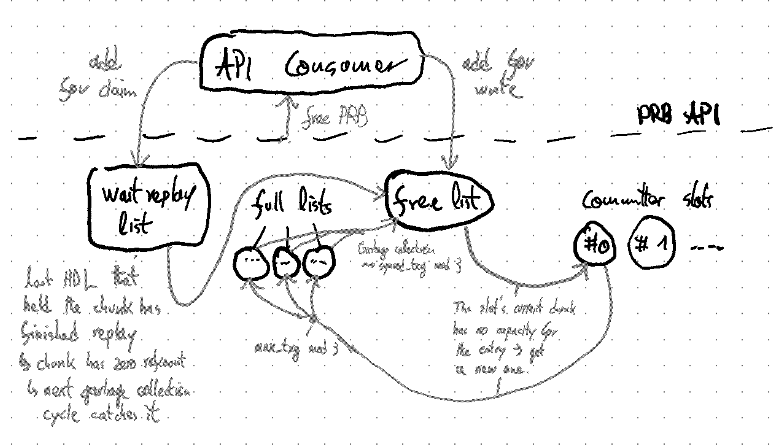
\includegraphics[width=\textwidth]{fig/prb_chunk_ownership_cycle__transitions}
    \caption{The different owners of a chunk and the events that cause ownership transitions.}
    \label{fig:prb_chunk_ownership_cycle__transitions}
\end{figure}

\begin{figure}[H]
    \centering
    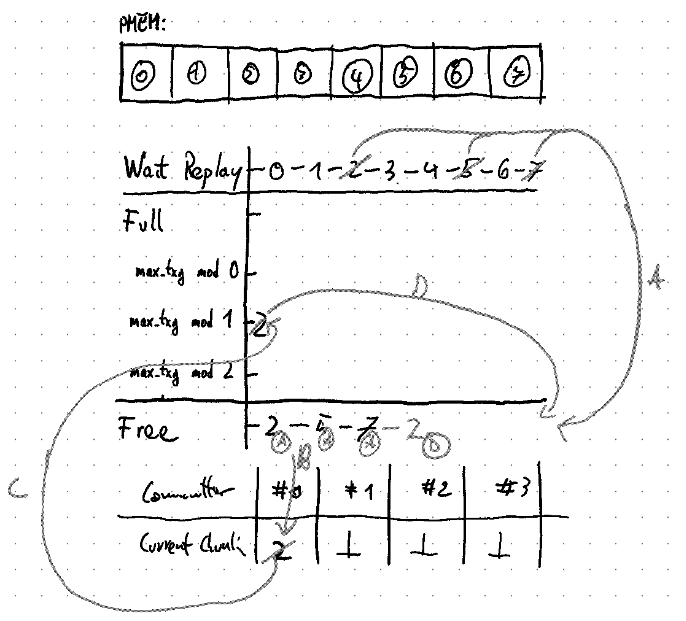
\includegraphics[height=12cm]{fig/prb_chunk_ownership_cycle__example}
    \caption{
        Example for chunk ownership transitions.
        The PRB is constructed with all eight chunks added as \lstinline{_for_claim}.
        Claiming (\textit{A}) determines that chunks 0, 1, 3, 4, and 6 need to remain on the \textit{wait replay list} because they contain entries for HDL logs that need replay.
        Chunks 2, 5, and 7 only contain obsolete entries and move to the \textit{free list}.
        We do not replay any of the logs.
        However, a log writer starts writing a new log in \textit{B}.
        It finds that its commit slot (\#0) has no active chunk.
        Thus, it and moves the first chunk on the \textit{free list} (i.e., chunk 2) to the commit slot.
        After writing the entry to chunk 2 the log writer releases the commit slot.
        Another log writer aquires commit slot \#0 and writes entries to it.
        Chunk 2's capacity is insufficient to hold the last entry (\textit{C}).
        The thread places chunk 2 on the correct \textit{full list} for chunk 2's \textit{max txg} and finds a new chunk on the free list for the commit slot (not shown).
        Eventually \textit{txg sync} triggers garbage collection for the txg that is chunk 2's \textit{max txg} which resets chunk 2's in-PMEM and in-DRAM sequence and subsequently places it back onto the free list.
    }
    \label{fig:prb_chunk_ownership_cycle__example}
\end{figure}

\section{PRB: PMEM Data Structure}\label{di:prb:pmemdatastructure}
As explained in the previous section, PRB is built on top of contiguous slices of PMEM which we call \textit{chunks}.
However, PRB only consumes the chunks, it does not create them.
Chunk allocation is the responsibility of the PRB consumer, i.e., ZIL-PMEM.
This design improvides modularity and testability because it decouples the following two concerns:
\begin{description}[noitemsep,leftmargin=1.5cm,labelindent=1cm]
    \item[Resource Aquisition] The PRB consumer is responsible for integrating PMEM SLOG vdev into the zpool, discovering its memory mapping, and partitioning the PMEM space.
    \item[PMEM Data Structure] PRB only implements the persistent data structure that stores entries in the chunks (next section\todo{ref}).
\end{description}
With regards to persistent data structure, this separation of concerns relieves PRB from the need to define structures to track the partitioning of PMEM space into chunks.
It relies on the consumer to provide the PRB with the same set of chunks every time the PRB is constructed.
% Our implementation of ZIL-PMEM uses a simplistic partitioning scheme.
% It uses a hard-coded chunk size of \SI{128}{MiB}\todo{check} and partitions as an array the allocatable into contiguous segments of that size.
% However, future work 
% \todo{future work: dynamically add and remove chunks}

% When the PRB is constructed, i.e., when the PMEM SLOG vdev is added to the pool, the consumer initializes the PMEM structure in each chunk before passing them to PRB.
% At all subsequent times when the PRB is constructed, the consumer must pass the same PMEM chunks to PRB's constructor function.
% More precisely, the start addresses of the PMEM chunks are allowed to change but their effective PMEM address range must be the same every time the PRB is constructed.

Entries are variable-length records that are stored within the chunk as a contiguous sequence.
Each entry is represented as a fixed-length 256 byte sized header and a variable-length body.
The first entry starts at the chunk's start address which must be algigned to 256 bytes.
The space after each entry is zero-padded to the next multiple of 256 bytes.
The next entry starts after the padding.
The sequence is terminated either explicitly by an invalid entry header or implicitly if the last entry has filled the chunk completely.
Figure~\ref{fig:prb_physical_data_structure__chunklayout} provides an example chunk layout.
Note that the ordering of entries within the chunk is has no semantic value as the logical view on the chunk is that of a set of entries.

The entry body is a verbatim copy of an opaque byte slice provided by the log writer.
(In ZIL-PMEM, this byte slice is the log record structure that is shared among all ZIL kinds.)
The entry header's contents are managed by the PRB and HDL.
Its contents are as follows:\todo{language}
\begin{description}[noitemsep,leftmargin=1.5cm,labelindent=1cm]
    \item[HDL-scoped metadata] The metadata required for attribution of a log entry to a HDL and subsequent replay.
    \begin{itemize}
        \item Log GUID
        \item Generation
        \item Geneneration-Scoped ID
        \item Encoded Counters for dependency tracking.
    \end{itemize}
    \item[Body Length] We store the exact body length in bytes.
    The zero padding in the chunk sequence is not considered part of the entry itself.\todo{fix that?}
    \item[Body Checksum] Fletcher checksum of the body data.
    \item[Header Checksum] Fletcher checksum of the header to ensure data integrity of the metdata.
    If the header checksum is corrupted then none of the other header fields can be trusted.
    \item[Zero Padding] The unused bytes in the header have the defined value of zero.
    Their value is part of the header checksum.
\end{description}

Chunks must be sufficiently large to hold at least one entry because there is no mechanism to split an entry across multiple chunks.
The smallest chunk's size determines the maximum entry size that can be written to it.
However, chunk sizes much larger than a single average entry are advisable for multicore-scalability, as we will elaborate on in Section~\ref{di:prb:write}.
%The choice of chunk size is a trade-off between PMEM space-efficiency (fragmentation at the end of the chunk), the acceptable blast radius\todo{this is a common ops term but not sure if academic enough...} of data corruption (traversal, see Section~\ref{di:prb:traversal}), and multi-core scalability on the write path (see Section~\ref{di:prb:write}).

\begin{figure}[H]
    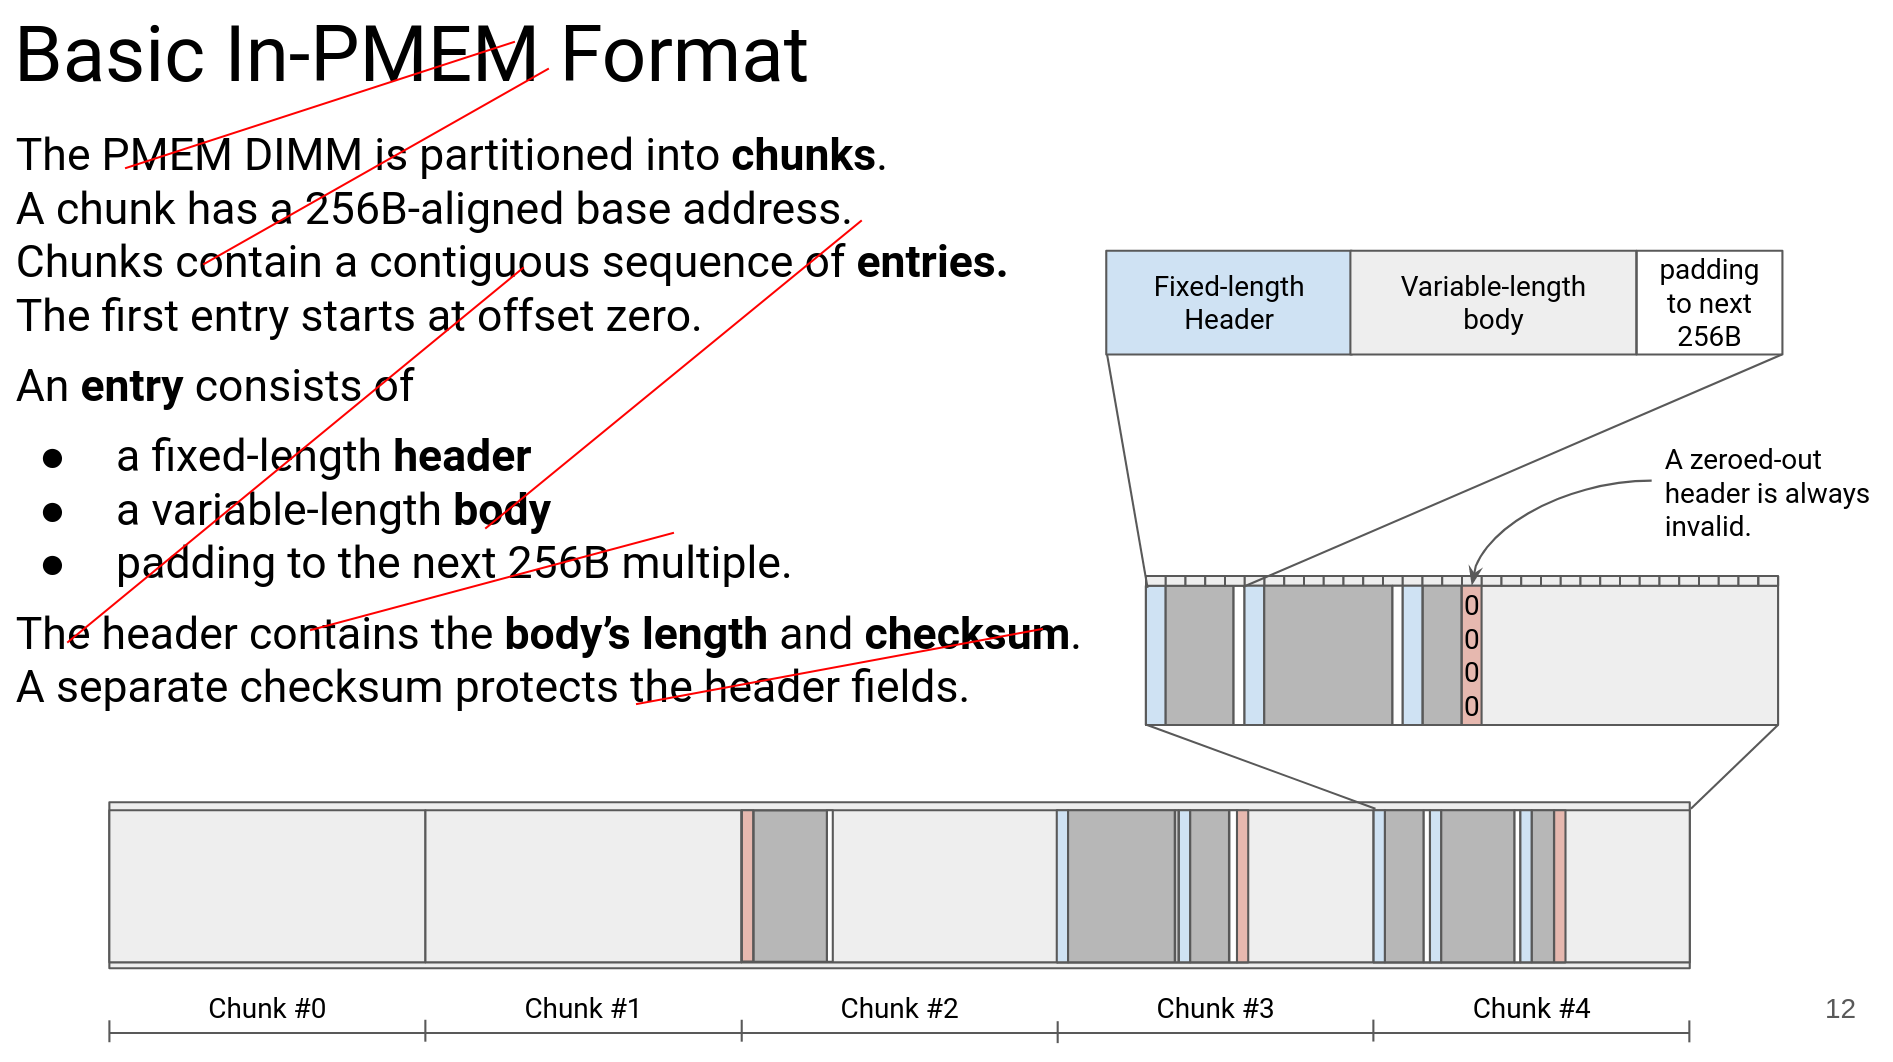
\includegraphics[height=7cm]{fig/prb_persistent_structure__chunklayout}
    \caption{Example chunk layout. Note that although we partition the PMEM space very regularly in this example, the PRB consumer is free to use variable-sized chunks.}
    \label{fig:prb_physical_data_structure__chunklayout}
\end{figure}


\section{PRB: Chunk Traversal}\label{di:prb:traversal}
HDLs scan the PRB during claiming to put their holds on chunks that contain replayable log entries.
During replay, the HDLs scan their held chunks again to construct the replay sequence.
The building block for both procedures is the iteration over the entries of a chunk.
We call this iteration process \textit{chunk traversal} and present the algorithm in this section.

As a reminder, the data layout within the chunk is as follows:
\begin{itemize}[noitemsep]
    \item The first entry header starts at chunk offset zero. Its size is fixed (256 bytes).
    \item The variable-length body starts immediately after the header. Its length is stored in the header.
    \item The body is followed by zero padding to the next 256 byte multiple.
    \item The next entry's header starts there.
    \item An invalid header marks the end of the chain.
        A header is invalid if its header checksum is invalid, or if the log GUID is invalid.
        The (128 bit) log GUID is invalid if at least the upper or lower 64 bits are zero.
    \item Entries are never split between chunks.
\end{itemize}

In the absence of data corruption in PMEM, chunk traversal visits each valid entry in the sequence and stops at its end.
For the case where PMEM is corrupted, we distinguish the following conditions\todo{word?}:
\begin{description}
    \item[Machine check exception (MCE)] If the PMEM hardware detects uncorrecta\-ble data corruption, it raises an MCE.
        The Linux kernel provides the an API (\lstinline{memcpy_mcsafe}) which provides a memcpy-compatible interface but converts MCEs into error return values.
        We always use this API to buffer PMEM contents in DRAM before accessing them.
        The error handling for MCE errors is the same as for invalid checksums in entry header and body, which we describe below.
    \item[Header: Detected Data Corruption]
        If the header checksum validation fails, the header was either corrupted by bitflitps or similar phenomena or never completely written.
        The latter case is critical for crash consistency on the write path as we will elaborate on in Section~\ref{di:prb:write:crashconsistency}.
        Regardless of the cause, an invalid header's values cannot be trusted, and thus the traversal stops.
    \item[Header: Undetected Data Corruption]
        If the header checksum does not detect data corruption in the header, the behavior is implementation defined.
        However, it is guaranteed that memory accesses are constrained to the entry's chunk's bounds.
    \item[Data corruption in the body]
        The traversal algorithm does not read the body but instead returns a closure that can be invoked for this purpose.
        The closure reads the body into DRAM using \lstinline{memcpy_mcsafe}, then validates the body checksum stored in the header.
        Validation failures are returned as an error.
        The caller can decide whether they want to iterate further or propagate the error up the call stack.
        Note that in our C implementation, the closure is replaced by the opaque struct \lstinline{zilpmem_replay_node_t} and function \lstinline{zilpmem_prb_replay_read_replay_node}.
    \item[Data corruption in the padding]
        We require that the padding in the space that follows the body to the next 256 byte multiple consists only of zero.
        We validate this property in the closure that reads the body.
        Validation failure results in a distinguished error being returned from the closure.
        Such an error is indicative of data corruption or an incorrect implementation on the write path.
        The caller of the traversal algorithm should surface it to the administrator, but may choose to proceed.
\end{description}

The following listing provides the pseudo code for chunk traversal.
\begin{lstlisting}[style=figurepseudocode]
Algorithm: iter_chunk() - Iterate over the entries in a chunk.

Inputs:

    ch_base    chunk's base address
    ch_len     chunk's length

Procedure:
    assert ch_base % 256 == 0
    assert sizeof(entry_header_t) == 256
    assert ch_len >= 256
    assert ch_len % 256 == 0

    e := ch_base
    while (e < ch_base + ch_len) {
        entry_header_t eh;

        // read header with a function that handles MCEs
        memcpy_mcsafe(&eh, e, sizeof(eh))?;

        // invalid hdr checksum or id terminate the sequence
        validate_header_checksum(eh)?;
        if eh.log_guid's upper or lower 64 bits are zero {
            return None;
        }

        body_ptr := e + sizeof(eh);

        if body_ptr + eh.body_len > ch_base + ch_len {
            return Err("""
              entry out of chunk boundary:
                a) writer implementation error
                b) undetected header corruption
            """);
        }
        e += sizeof(eh) + body_len;
        e = roundup_to_next_256byte_multiple(e);

        padding_ptr := body_ptr + eh.body_len
        padding_len := e - padding_ptr

        read_body := |buffer: *u8| {
            memcpy_mcsafe(buffer, body_ptr, eh.body_len)?;
            validate_body_checksum(eh, buffer, eh.body_len)?;
            pmem_is_zero(padding_ptr, padding_len)?;
            return Ok(());
        };
        yield Some((eh, read_body))
    }

Example:

    for (entry_header, read_body) in iter_chunk(...) {
        if entry_header.txg <= precrash_txg {
            continue;
        }
        buf := buffer of size entry_header.body_len
        read_body(buf)?;
        ...
    }
\end{lstlisting}

\section{PRB: Garbage Collection}\label{di:prb:gc}
We already covered the essence of garbage collection in Section~\ref{di:prb:dramdatastructure}:
if the capacity of an acquired commit slot is insufficient, the log writer puts it on the \textit{full list} for the chunks' \textit{max txg} and gets a new chunk from the \textit{free list}.
After \textit{txg sync} has written out that \textit{max txg}, it triggers garbage collection, which removes all entries in the chunks on the \textit{full list} for \textit{max txg}.

We remove all entries in a chunk in $O(1)$ time by invalidating the log GUID in the first entry header in the chunk (offset zero).
As indicated by the This is sufficient to prevent chunk traversal in the future.
The pseudo-code to invalidate a chunk is as follows:

\begin{lstlisting}[style=figurepseudocode]
Input:
    ch_base     chunk base address
    ch_len      chunk length
Steps:
    assert ch_len >= 256

    assert type of entry_header_t::log_guid is uint64_t[2]

    log_guid_addr := ch_base + offsetof(entry_header_t, log_guid)

    assert log_guid_addr is 64-bit aligned

    atomic 64-bit store of 0 to log_guid_addr
    atomic 64-bit store of 0 to log_guid_addr + 8

    flush modified cache lines
    sfence
\end{lstlisting}

\section{The Write Path}\label{di:prb:write}
A thread that writes an entry to a HDL needs to perform the following tasks:
\begin{itemize}[noitemsep]
    \item Find a target chunk using the \textit{commit slot} mechanism. (Section~\ref{di:prb:write:chunksel})
    \item Determine the HDL-scoped metadata, i.e., log GUID, txg, gen, gsid, and counters.
    \item Compute header and body checksums.
    \item Insert the entry into the target chunk in a crash-consistent manner.
\end{itemize}
Our goal is a design with low write latency, good multicore-scalability, and CPU efficiency.
We identify the following factors as particularly relevant:
\begin{description}[noitemsep]
    \item[Checksumming] Checksumming adds latency but does not concern multicore scalability since no coordination is required between writers.
        The implementation should use ZFS's optimized implementations of the Fletcher checksum.
    \item[Dependency Tracking Counters] We must update the dependency-tracking counters on every entry write operation.
        Since the counters are HDL-scoped, this only presents a scalability concern if a single HDL is written from multiple threads.
        Parallel writes to the same HDL do not happen in ZIL-PMEM proper but are relevant for our ZVOL-specific ITXG bypass (Section~\ref{sec:itxgbypass}).
    \item[Commit Slot Aquisition \& Chunk Replacement]
        The PRB's commit slots and chunk lists are shared among all HDLs.
        All threads that write to any HDL of the PRB compete for these resources, making it a multi-core scalability challenge.
    \item[Optane Characteristics] We develop and evaluate ZIL-PMEM for/on Intel Optane DC Persistent Memory.
        The performance characteristics of Optane DIMMs are significantly different from regular DRAM.
        \citeauthor{yangEmpiricalGuideBehavior2020} have established that the Optane PMEM hardware is organized in units of 256 bytes.
        For example, the access granularity and kind of store and cache flush instruction have significant impact on the achievable write bandwidth.
        For size of log entries written by ZIL-PMEM, the use of  AVX-512 non-temporal store instructions is recommend for highest possible performance.~\cite{yangEmpiricalGuideBehavior2020}.
    \item[PMEM Bandwidth Limits \& Multicore Scalability]
        It is inherent to the programming model for persistent memory that wait time for PMEM I/O is spent on-CPU.
        For example, instructions that architecturally depend on a preceding store+cacheflush+sfence to PMEM will stall until the flushed cacheline reaches the power-fail protected domain of the CPU~\cite{Scargall2020}.
        This is problematic from a CPU utilization perspective:
        if multiple threads attempt to write at higher bandwidth than PMEM can sustain, they still appear busy towards the OS thread scheduler and waste CPU time that could be used more productively by other threads in the system.
        \citeauthor{yangEmpiricalGuideBehavior2020} have shown that a single Optane DIMM's write bandwidth can be exhausted by one CPU core at \SI{2}{GB/s}.
        Write bandwidth decreases to \SI{1}{GB/s} at ten or more concurrently writing CPU cores ~\cite{yangEmpiricalGuideBehavior2020}.
        Whereas excessive on-CPU waiting might be the right trade-off in certain userspace applications of PMEM, a kernel file system such as ZFS cannot make assumptions about the system's overall CPU priorities.
        We expect that PMEM write bandwidth can be exhausted in real-world use cases for ZIL-PMEM.
        Our design must therefore find a way to limit concurrent access to PMEM and shift PMEM wait time off the CPU.
\end{description}

\subsection{Commit Slots}\label{di:prb:write:chunksel}
Commit slots are our abstraction to enable multiple threads to write entries concurrently.
The goal is to grant up to \lstinline{ncommitters} parallel writers temporary exclusive access to a chunk into which they can write their log entry.
For this purpose, a thread that wants to write an entry \textit{aquires a commit slot} $S \in {0, 1, \dots, ncommitters-1}$.
Each thread that is simultaneously committing gets a different commit slot.
If no commit slot is available, the function to aquire the commit slot blocks.
Associated with each commit slot is a PMEM chunk which we refer to as \textit{open chunk}.
A thread that aquires a commit slot is allows to write its entry to the slot's \textit{open chunk}.

The limitation to \textit{ncommitter} parallel writers is desirable to avoid excessive on-CPU waiting on PMEM.
Let us make the simplifying assumption of a fixed maximum write bandwidth of $B_max [byte/s]$ to PMEM before latency increases dramatically due to queuing.
Then an equal distribution of that bandwidth yields $\frac{B_max}{ncommitters} [byte/s]$ of write bandwidth per writer.
Assuming that writers do not exceed this limit, we can derive latency guarantees for writing entries, dependent on entry size.

We implement commit slots using a semaphore initialized to \textit{ncommitters} and a bitmask with \lstinline{ncommitters} bits.
The thread that aquires a commit slot first enters the semaphore and then finds and flips a zero bit in the bitmask.
The zero bit's index is the commit slot number.
We use opportunistic spinning to find and flip the bit.
The following pseudo-code explains the aquisition and release procedures.

\begin{lstlisting}[style=figurepseudocode]
Procedure For Commit Slot Aquisition:
  Input:
      sem     semaphore
      bm      pointer to PRB-wide bitmask with ncommitters bits
  Output:
      The commit slot number.
  Steps
    Enter semaphore.

    my_bm   <-  atomic_load(bm, SeqCst)
  'retry:
    idx     <- find first set bit index in (~my_bm)
    if idx == 0:
        panic: idx=0 indicates there is no free bit,
               but the semaphore guarantees that
    idx -= 1
    if idx >= ncommitters:
        panic: semaphore guarantees that there are
               free commit slots

    my_bm = my_bm | (1<<idx)
    if compare_and_swap(bm, &my_bm, SeqCst):
        // we won the race => return the commit slots
        return idx
    else:
        // we lost the race with another committer
        // => retry
        // (my_bm contains the actual value of bm)
        goto retry

---

Procedure For Commit Slot Release:

  Input:
      cslot     The commit slot number returned on aquisition.
  Steps:
    Atomic bitwise and of bm with ~(1<<idx)
    Exit Semaphore
\end{lstlisting}

The procedure above is all the PRB-wide coordination that is required for writing a log entry, iff the aquired slot's \textit{open chunk}'s capacity is sufficient.
If capacity is insufficient, the writing thread replaces the full \textit{open chunk} with a new one.
To accomplish that, it puts the current \textit{open chunk} on the correct \textit{full list} and gets a new \textit{open chunk} from the \textit{free list}.
Access to the PRB's lists is protected by a PRB-wide mutex.
The potential contenders for this mutex are up to \textit{ncommitters} writer threads and the txg sync thread that performs garbage collection.

Getting a new chunk from the \textit{free list} fails if the free list is empty.
The log writer can choose whether to block and wait or fail the log entry write operation with an error.
Block-and-wait is implemented through a condition variable that is signalled by garbage collection for every chunk that it puts back on the \textit{free list}.
If the log writer chooses to block and wait during chunk replacement, it must guarantee that it does not prevent \textit{txg sync} from making progress in order to avoid a pool-wide deadlock.
In practice, this means that the log writer must not hold a DMU transaction open when writing an entry.
Note that this is the case for ZIL-PMEM proper because \lstinline{zil_commit} is called after the DMU transactions have finished or failed.
However, for the ITXG bypass for ZVOLs (Section~\ref{sec:itxgbypass}\todo{chapter?}), we write log entries from within the DMU transaction and thus need to use the non-blocking mode.

Sharing the slots (and thus chunks) among all threads and HDLs in the PRB is of ambiguous value from perspectives other than bandwidth limitation:
\begin{description}
    \item[Space Efficiency]
        Sharing chunks causes entries to be packed into a small number of chunks, even more so if we implemented some form of \textit{best fit} selection scheme for commit slots.
        Packing is beneficial for space efficiency because the \textit{spread} between mininum and maximum txg of the entries in a chunk is small, enabling timely garbage collection.
        \todo{one sentence on limited slog size, that it's not as relevant for PMEM, but maybe for NVDIMM-N?}
    \item[Blast Radius]
        However, the concentration of entries in a chunk also increases the blast radius of data corruption due to the chunk's physical data structure which we discuss in Section~\ref{di:prb:pmemdatastructure}.
        In particular, data corruption within the entry metatadata of one HDL's entry can render another HDL's entry unreachable during PRB scan if they are stored in the same chunk.
    \item[Cache Efficiency] Our aquisition procedure deterministcally picks the lowest available commit slot.
        It is thus very likely that chunks bounce around CPU cores, without taking temporal locality into account.
        Note that, due to the use of non-termporal store instructions when writing log entries to PMEM, this only impacts the chunk DRAM object.
        We briefly experimented with per-core commit slots during development and found no noticable performance difference to the approach presented above.
\end{description}
\todo{this last paragraph doesn't feel right here...}

\subsection{HDL-Scoped Metadata}\label{di:prb:write:hdlscoped}
We have already-addressed the algorithm to compute the HDL-scoped entry metadata (Log GUID, txg, gen, gsid, Counters Table) in Section~\ref{di:prb:recovery}\todo{check matches}.
This subsection only addresses multithreading and scalability concerns.

First of all, HDL-scoped metadata does not pose a scalability concerns if entries are written sequentially.
This is the case for ZIL-PMEM proper which uses a mutex to serialize \lstinline{zil_commit} calls.
(Remember from Section~\ref{di:prb:background} that the ZIL's shared itxg structure defines the sequential \textit{commit list} model.)
However, for the ITXG bypass for ZVOLs (Section~\ref{sec:itxgbypass}), the ZVOL dataset's HDL can be written in parallel.

Multiple threads are allowed to write to a single HDL simultaneously iff they do not start a new generation.
Threads that start a new generation must wait for all threads that wrote entries to the previous generation to finish writing.
The reason is that the new generation's entry logically depends on the previous generation's entry.
It would be sufficient to prevent the \textit{function calls} from returning out of dependency order while allowing the new generation's entry to be written in parallel with the old entries.
Such a system is used by ZIL-LWB's \textit{commit ITXs} which uses condition variables to wake \lstinline{zil_commit}ting threads up when the last LWB that contains one of their commit list's records has been written.
However, the \textit{commit ITX} model was not directly applicable to ZIL-PMEM proper.
For the ITXG bypass, we use a simple read-write-lock which we elaborate on in Section~\ref{sec:itxgbypass}.\todo{check content}

Within the HDL, we use a spinlock to serialize access to the state used for dependency tracking (\textit{live table}, \textit{last table}).
We only compute the encoded representation of the \textit{last table} when the first entry is counted for a new generation.
Subsequent writes for the same generation only need to \lstinline{memcpy} the pre-computed encoded representation while holding the spinlock.

\subsection{Crash-Consistent Insert}\label{di:prb:write:crashconsistency}
After the commit slot has been aquired, a target chunk been selected, and the HDL-scoped metadata determined, we are ready to insert the entry into the chunk.
Remember from Section~\ref{di:prb:pmemdatastructure} that the chunk is a sequence of entries that is terminated by an invalid entry header.
To insert the entry into the chunk, we must append the entry to the sequence in a way that is crash-consistent with regards to the traversal algorithm (Section~\ref{di:prb:traversal}):
\begin{displayquote}
    Appending an entry $E_{n+1}$ to a chunk $C$ that contains a sequence of entries $E_1,~\dots,~E_n$ must be atomic from the perspective of traversal.
    After a system crash or power failure during the append operation, traversal of $C$ must either find $E_1,~\dots,~E_n$ or $E_1,~\dots,~E_n,~E_{n+1}$.
\end{displayquote}
The following algorithm describes the procedure and invariants during the append operation.
Figure~\ref{fig:prb_writepath_crashconsistent_append} contains a step-by-step visualization.
\begin{lstlisting}[style=figurepseudocode]
Inputs:
    ch  The chunk into which we append
    e   The entry that we append to ch's sequence.
Procedure:
  Invariant 1: Traversal will stop at ch.pos because
               either: ch.pos points to PMEM space that
                       is an invalid header
               or: there is no space left in the chunk

  Phase 1:
    Write e.body to address ch.pos + 256
    Write trailing zero padding
    If there is still space in the chunk at
      address ch.pos + 256 + e.body_len + padding_len:
        Assert that the space is at least 256 bytes.
        Write an invalid follow header (256 zero bytes)
          to that address.
    Cacheflush + Sfence

  Corrolary 1: Neither body nor follow header
               will be visited by traversal
               because traversal still stops
               at address ch.pos (Invariant 1).

  Phase 2:
    Write e.header (256 bytes) to address ch.pos
    Cacheflush + Sfence

  Corrolary 2: Traversal visits the entry written
               to ch.pos and stops at the follow
               header.
\end{lstlisting}
Invariant 1 can be proven by induction:
if the entry being written is the first entry in the sequence (base case) the chunk was fetched from the \textit{free list} which is defined to only contain chunks that are \textit{empty}.
(\textit{Empty} means that the write position (\lstinline{ch.pos}) is at the chunk's base address and that the PMEM at the write position is an invalid header.)
% The induction step is that if invariant 1 holds for a sequence with entries $E_1~\dots~E_n$, it also holds for a sequence with entries $E_1~\dots~E_{n+1}$.
The induction step is that if an entry $E_{n+1}$ is appended to an existing sequence $E_n$, invariant 1 holds as well.
This is true because the space occupied by $E_{n+1}$ contains an invalid follow header written by phase 1 when $E_n$ was appended to the sequence.
Stores made in Phase 1 for $E_n$ are guaranteed to be persistent before any store for $E_{n+1}$ happens due to the \lstinline{cacheflush+sfence} at the end of Phase 1.
Note that we do not need to address the case where the chunk is full because we cannot append $E_{n+1}$ to a full chunk.

The first \lstinline{sfence} in phase 1 is required for correctness iff we do not trust the body checksum to detect partial writes.
If we omitted the \lstinline{sfence} in phase 1, it would be possible that the entry header written in phase 2 reaches PMEM completely but the body written in phase 1 does not.
In that case, after a crash, the traversal algorithm would observe a valid header but a body space with undefined content.
We would rely fully on the body checksum to detect the partially written body.
If the checksum is too weak, the replayer's interpretation of the undefined body contents determines subsequent behavior.
Corruption of the dataset is a likely consequence.

The \lstinline{sfence} (phase 2) is required for correctness  because we must conservatively assume that the log writer's subsequent store instructions (in program order) depend on the entry having reached stable storage.

\begin{figure}[H]
    \centering
    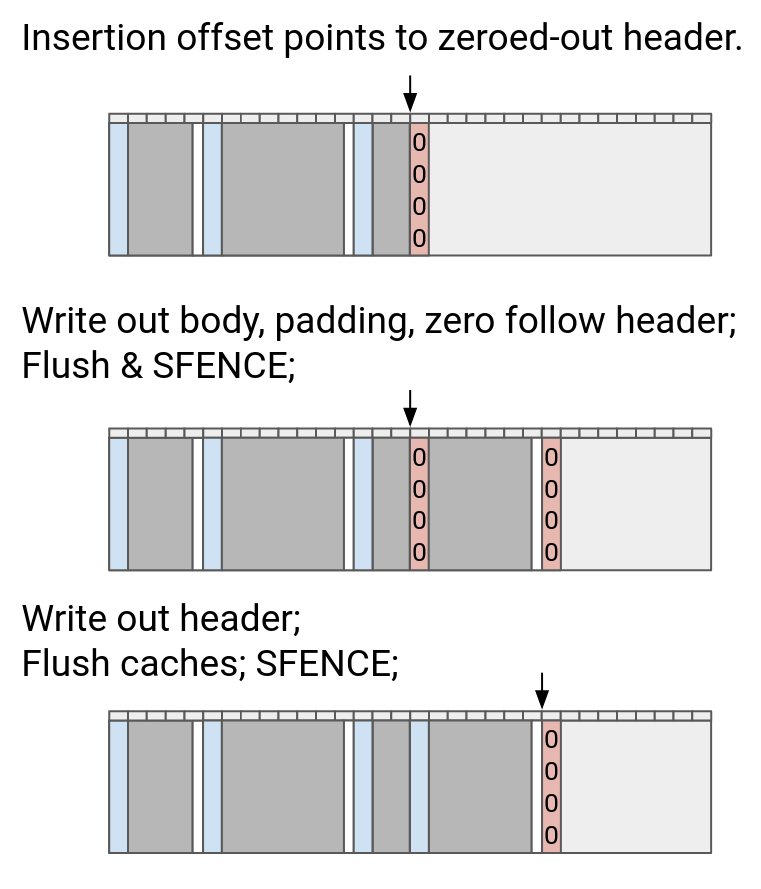
\includegraphics[height=6cm]{fig/prb_writepath_crashconsistent_append}
    \caption{
        The crash-consistent append operation to a PMEM chunk.
        The traversal algorithm reaches the existing entries at all times and reaches the new entry only after its body and header have been written completely.
    }
    \label{fig:prb_writepath_crashconsistent_append}
\end{figure}

The following implementation details of the append operation are relevant for latency and efficient use of CPU time:
\begin{itemize}[noitemsep]
    \item For ZIL-PMEM, the use of \lstinline{sfence} in phase 1 came with negligible impact on overall latency during development.
        We assume that this is because the wait time added by the \lstinline{sfence} is neglible compared to the write time for the entry body.
        For example, the entry body and zero padding for a 4k sync write is $sizeof(lr_write_t) + data + padding = 4096 + 192 + 64 = 4352$ bytes large.
        Assuming \SI{2}{GiB/s} write bandwidth for a single Optane DIMM \cite{yangEmpiricalGuideBehavior2020}, the write time for the entry body is $\sim$~\SI{2}{us}.
        In contrast, the derived latency for a 256 byte write at that rate is $\sim$~\SI{0.12}{us}.
        If we use this value as an approximation for the cost of the \lstinline{sfence}, its latency contribution is only $\frac{0.12}{0.12 + 2} = 5.6\%$.
    \item All writes to PMEM happen in multiples of 256 bytes because 256 bytes is Optane's internal write unit size.
        Writes below this size cause read-modify-write cycles in the hardware and thus cost performance~\cite{yangEmpiricalGuideBehavior2020,zhangChameleonDBKeyvalueStore2021}.
    \item We use AVX-512 non-temporal store instructions (\lstinline{movnt}) instead of regular stores and cache flushes.
        Again, this addresses established performance properties of Intel Optane DC Persistent Memory~\cite{yangEmpiricalGuideBehavior2020}.
    \item We also use ZFS's optimized implementation of the Fletcher checksum to compute body and header checksums.
        Whereas the best implementation is chosen by benchmark dynamically at runtime, it is safe to assume that some SIMD ISA extension such as AVX-512 will be used if available.
    \item OpenZFS cannot rely on the Linux kernel's interface for saving FPU state due to licensing issues~\cite{LinuxCompatSIMD}.
        Unless the FPU is used by a dedicated kernel thread, ZFS must temporarily disable preemption, mask local interrupts, and manually save FPU state.
        PRB is written directly from the task that calls \lstinline{zil_commit} and thus incurs this overhead.
        We refactor ZFS's FPU state management abstraction so that FPU context is only saved once for both checksum computation and writing to PMEM.
        The time that is spent in this suboptimal state is bounded by the maximum log entry size.
        \todo{we have no evaluation on impact of interrupt masking, future work}
\end{itemize}

%Note that a fully sequential chain of entries is sufficient for today's ZIL since the commit list assembled by the ITX code\todo{ref} is already sequential.
%However, as pointed out by the example in the previous paragraph, full sequentiality is not always semantically necessary.
%This observation has already led to a prototype design for ZIL-LWB that allows for more parallel I/O if the entries in written LWBs are not interdependent~\cite{openzfsZILPerformanceImprovements2020}.
%We interpret these findings as indicators that ZIL-PMEM --- and thus PRB --- should support parallelism on the write path in the form of diamond chains.
%We present an application of diamond chains to ZVOLs in Section~\ref{sec:itxgbypass} and evaluate it in Section~\ref{ch:eval}\todo{precise}.

%A generation is identified by its \textit{generation number} which is positive integer.
%An entry is always associated with exactly one generation but a generation can contain many entries.
%Entries within the same generation are identified through an \textit{id field} which is a positive integer.
%Given entries $a$ and $b$, $a \text{depends on} b \Leftrightarrow a.gen > b.gen$ where $x.gen$ denotes the generation of entry $x$.

\section{API Design}\label{di:prb:api} % API Overview?
We briefly discuss the PRB/HDL API that is used by the \texttt{zil\_pmem.c} module.
In the implementation, most types and functions are prefixed with \lstinline{zilpmem_} or \lstinline{zilpmem_prb_t} which we omit for brevity.

\subsection{PRB Setup}
\begin{lstlisting}
prb_t* prb_alloc(size_t ncommitters);
void prb_free(prb_t *b, bool free_chunks);

chunk_t* chunk_alloc(uint8_t *pmem_base, size_t len);
void chunk_free(chunk_t *c);

void prb_chunk_initialize_pmem(chunk_t *c);
void prb_add_chunk(prb_t *prb, chunk_t *chunk);
\end{lstlisting}

The zpool import procedure allocates the PRB using the \lstinline{prb_alloc} function.
The returned \lstinline{prb_t} is owned by the caller which is responsible for freeeing it using \lstinline{prb_free} during pool export.

The PRB consumer allocates the chunk objects using \lstinline{chunk_alloc}.
It adds the chunk to the PRB using \lstinline{prb_add_chunk}.
The PRB assumes ownership of the chunks that are added to it.
When the PRB is constructed for the first time, the PRB consumer must call \lstinline{prb_chunk_initialize_pmem} to reset the PMEM sequence to an empty state.

The \lstinline{free_chunks} argument to \lstinline{prb_free} determines whether the PRB should free the chunks objects that were added to it, or whether the ownership moves back to the caller.
Note that freeing the chunk object (\lstinline{chunk_free}) does not alter the chunk's PMEM state.

\subsubsection{HDL Setup}\label{di:prb:api:hdl}
\begin{lstlisting}
void zil_header_pmem_init(zil_header_pmem_t *zh);
hdl_t* prb_setup_hdl(prb_t *prb, const zil_header_pmem_t *hdr);
void prb_teardown_hdl(hdl_t *hdl,
    bool abandon_claim, zil_header_pmem_t *upd);
\end{lstlisting}

HDL recover their DRAM state from the ZIL header (\lstinline{zil_header_pmem_t}).
The setup \lstinline{prb_setup_hdl} function takes a constant pointer to the last-synced header.
The pointer is not internalized in HDL --- the pointee's lifetime may be as short as the function call.
The PRB consumer instantiates all dataset's HDLs during pool import or whenever a new dataset is created.
For new datasets, the initial value for the ZIL header (state \textit{nozil}) is set by \lstinline{zil_header_pmem_init}.

When the head dataset is destroyed or the pool is exported, the PRB consumer calls \lstinline{prb_teardown_hdl} to destroy the HDL.
The PRB must be freed before all of its HDL's have been torn down.

\subsubsection{Claiming}\label{di:prb:api:claiming}

\begin{lstlisting}
check_replayable_result_t prb_claim(
    hdl_t *hdl, uint64_t pool_first_txg,
    zil_header_pmem_t *upd);
\end{lstlisting}
% NOTE: we omitted the whole claimstore stuff from the thesis because we rule out WR_INDIRECT support in the 'requirements' section.

After the PRB is constructed and HDLs are set up, we must \textit{claim} log entries of all dataset's HDLs.
The corresponding function \lstinline{prb_claim} is invoked by the pool import procedure for each HDL.
The \lstinline{pool_first_txg} is the pool's first new transaction group.
For HDLs in state \textit{logging}, \lstinline{pool_first_txg - 1} becomes the $precrash\_txg$.

\lstinline{prb_claim} returns an update to the ZIL header through the \lstinline{upd} out-parameter.
We employ this pattern throughout the entire PRB API.
It is always the API consumer's responsibility to ensure that the update is correctly persisted in the correct transaction group.

Claiming can fail, e.g., if the procedure detects a missing entry for the HDL (claiming performs a dry-run of replay internally).
The API consumer defines the error handling policy.
It can either abort pool import or choose to abandon the log.
To abaondon the log, the API consumer must first tear down the HDL using \lstinline{prb_teardown_hdl,  abandon_claim=true, ...)} to release claims made during \lstinline{prb_claim}.
Then, the API consumer resets the header using \lstinline{zil_header_pmem_init} and re-instantiates the HDL using \lstinline{prb_setup_hdl}.
\todo{need third option to retry with an override flag that discards the unreplayable part of the log}

After all HDLs have been claimed the pool import procedure starts \textit{txg sync} which writes out the header updates made by claiming in the \lstinline{pool_first_txg}.
From that point on there is no need to coordinate HDL operations between different datasets.

% Remember from Section~\ref{bg:zfs:logreplay} that ZIL replay can be deferred for an indefinite amount of pool import/export cycles and system shutdowns.
% Claiming scans the PMEM chunks that were added with \lstinline{zilpmem_prb_add_chunk_for_claim} for log entries that need to be replayed.
% Chunks that contain unreplayed log entries are not considered when writing new entries.

\subsection{Replay}\label{di:prb:api:replay}

\begin{lstlisting}
typedef struct { ... } replay_result_t;

replay_result_t
prb_replay(hdl_t *hdl, replay_cb_t cb, void *cb_arg);

typedef struct replay_node replay_node_t;
typedef int (*replay_cb_t)(void *rarg,
    const replay_node_t *rn,
    const zil_header_pmem_t *upd);

typedef enum {
	READ_REPLAY_NODE_OK,
	READ_REPLAY_NODE_MCE,
	READ_REPLAY_NODE_ERR_CHECKSUM,
	READ_REPLAY_NODE_ERR_BODY_SIZE_TOO_SMALL,
} read_replay_node_result_t;

read_replay_node_result_t
prb_replay_read_replay_node(
    const replay_node_t *rn,
    uint8_t *body_out, size_t body_out_size,
    size_t *body_required_size);

void prb_replay_done(
    hdl_t *hdl, zil_header_pmem_t *upd);

\end{lstlisting}

When a dataset is mounted the mounting procedure must always call \lstinline{prb_replay}.
If the HDL is in state \textit{nozil}, the call is a no-op.
If the HDL is in state \textit{replaying}, the function invokes the provided replay callback for each log entry that needs to be replayed in replay order.
The callback must perform the following steps for crash-consistent replay for each replayed entry $E$.
\begin{enumerate}[noitemsep]
    \item Start a DMU transaction $tx$.
    \item Load the entry $E$ into a DRAM buffer using \lstinline{prb_replay_read_replay_node}.
    \item Apply the change encoded in $E$ to the dataset.
    \item Update the ZIL header to the value of \lstinline{*upd}.
    \item \lstinline{dmu_tx_commit(tx)} the DMU transaction.
\end{enumerate}

Note that the callback must use \lstinline{prb_replay_read_replay_node} function because \lstinline{replay_node_t} is an opaque type in the PRB API.
The function forces the API consumer to do DRAM buffering and protects against online and offline data corruption internally, as dicussed in Section~\ref{di:prb:ccrecovery}.

\lstinline{prb_replay} can fail either due to an error returned by the callback, due to an error in the scanning phase, or due to log corruption.
If the error is due to missing log entries, the struct returned by the API contains the \textit{witness} log entry (see Section~\ref{di:prb:deptrack}).
The caller decides whether to retry replay or abandon the remaining unreplayable part of the log\todo{retry with an override flag that discards the unreplayable part of the log}.
End of replay must be acknowledged explicitly by calling \lstinline{prb_replay_done}.
Abandonding the log is done using \lstinline{prb_destroy_log} (next section).

%The invocation order corresponds to the order in which the entries were written.
%Entries that were written in parallel (\lstinline{needs_new_gen == false}) are replayed in a deterministic order to allow for resumability.

\subsection{Writing Entries}\label{di:prb:api:write}

\begin{lstlisting}
bool prb_create_log(hdl_t *hdl, zil_header_pmem_t *upd);
void prb_destroy_log(hdl_t *hdl, zil_header_pmem_t *upd);

int prb_write_entry(hdl_t *hdl,
    uint64_t txg, bool needs_new_gen,
    size_t body_len, const void *body_dram);
\end{lstlisting}

After successful replay, the HDL is always in the unwriteable state \textit{nozil}.
The log writer must use \lstinline{prb_create_log} to create a new log idempotently.
If the HDL is in state \textit{nozil}, the function alloctes a log GUID and transitions the HDL to state \textit{logging}.
Otherwise, the HDL must already be in state \textit{logging} and the call is a no-op.
If a new log was created, the caller must ensure that the transaction group that persists the ZIL header update has synced to disk before starting to write log entries.
The caller distinguishes the caes based on the function's return value.

Log writers use the \lstinline{prb_write_entry} function to write log records to the HDL.
The log record is treated as an opaque blob.
PRB does not provide facilities to version different version of the encoding.\todo{fix in upstream release?}
In addition to the body (\lstinline{body_dram}, \lstinline{body_len}), the log writer must provide two pieces of metadata:
\begin{description}[noitemsep,leftmargin=1.5cm,labelindent=1cm]
    \item[txg] The transaction group $T_{i_{txg}}$ of the DMU transaction $T_i$ whose changes $C_i$ are encoded in the log entry (Section~\ref{di:prb:structure}).
        Note: for ZIL-PMEM, this value is always the same as the log record's \lstinline{lrc_txg} field.
    \item[needs\_new\_gen] Indicates whether a new generation should be started for this log entry.
        It is the responsiblity of the caller to serialize the start of a new generation as described in Section~\ref{di:prb:write:hdlscoped}.
        if a thread writes an entry with \lstinline{needs_new_gen} is \lstinline{true}, that thread must be the only thread executing \lstinline{zilpmem_prb_write_entry} for the given HDL.
        The inverse\todo{contrary?} is not true: if \lstinline{needs_new_gen} is \lstinline{false}, multiple threads may write entries in parallel to the same HDL.
        Note that writers for different HDLs need not coordinate at all.\todo{language?}
\end{description}

\subsubsection{Garabge Collection}

\begin{lstlisting}
void prb_gc(prb_t *prb, uint64_t synced_txg);
\end{lstlisting}

Whenever \textit{txg sync} has finished syncing a txg $T$ to the main pool it must call \lstinline{prb_gc} with \lstinline{synced_txg = T}.
Note that unlike writing or recovering an individual log, garbage collection is a PRB-level operation.
Synchronization is handled internally.

% \subsubsection{ZIL header}\label{di:prb:persistent:zilheader}
% The ZIL header (\lstinline{zil_header_pmem_t}) is the persistent representation of the HDL state.
% Not every aspect of the runtime state of HDL is reflected in it, but only the information needed for claiming and replay.
% The ZIL header has the following states, some of which have associated data:
% \begin{description}[noitemsep,leftmargin=1.5cm,labelindent=1cm]
%     \item[nozil] There is no log for this dataset. (No associated data.)
%     \item[logging] The log has been created and entries might have been written to PMEM.
%         Claiming has never been attempted or never been completed.
%         The log remains in this state for the entire time until it is destroyed or the system crashes. Associated data: \textit{Log GUID}.
%     \item[replaying] The log has been claimed and replay is ongoing. Associated data: \textit{Log GUID} and \textit{serialized replay algorithm state}.
% \end{description}
% The diagram in Figure~\ref{fig:prb_persistent_structure__header_states_plus_example} visualizes the state transitions that the ZIL header goes through as the log is created, written and recovered.

% \begin{figure}
%     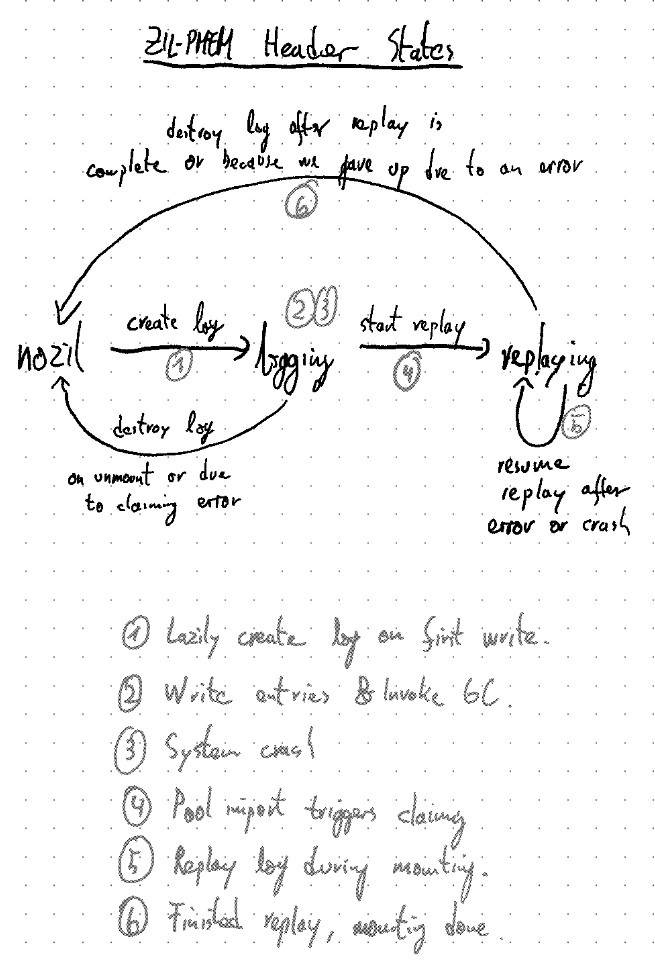
\includegraphics[height=15cm]{fig/prb_persistent_structure__header_states_plus_example}
%     \caption{
%         The states of \lstinline{zil_header_pmem_t} and the events that cause state transitions.
%         The grey annotations illustrates the path from log creation to finished recovery.}
%     \label{fig:prb_persistent_structure__header_states_plus_example}
% \end{figure}

% We use the following C structure to encode the ZIL header state.
% The \lstinline{zhpm_st} field is always valid and is one of \lstinline{ZHPM_ST_NOZIL}, \lstinline{ZHPM_ST_LOGGING}, or \lstinline{ZHPM_ST_REPLAYING}.
% The \lstinline{zhpm_guid_} fields are only valid in states \lstinline{ZHPM_ST_LOGGING} and \lstinline{ZHPM_ST_REPLAYING}.
% The \lstinline{zhpm_replay_state} is only valid in state \lstinline{ZHPM_ST_REPLAYING}.
% Hence we will describe its contents in Section~\ref{di:prb:recovery}.
% \begin{lstlisting}
% typedef enum zil_header_pmem_state {
%     ZHPM_ST_NOZIL,
%     ZHPM_ST_LOGGING,
%     ZHPM_ST_REPLAYING,
% } zil_header_pmem_state_t;

% typedef struct zil_header_pmem {
%     uint64_t zhpm_st; /* zil_header_pmem_state_t */
%     uint64_t zhpm_guid_1;
%     uint64_t zhpm_guid_2;
%     zilpmem_replay_state_phys_t zhpm_replay_state;
% } zil_header_pmem_t;
% \end{lstlisting}





% \subsubsection{Replay Sequence Algorithm}
% The basis for claiming and replay is the \textit{replay sequence algorithm}.
% Its inputs are the HDL's log GUID, a set of \lstinline{prb_chunk_t} references, and a callback.
% The algorithm consists of a \textit{scanning phase} and an \textit{iteration phase}.
% The scanning phase uses the traversal algorithm (Section~\ref{di:prb:traversal}) to search for log entries that have the HDL's \textit{log GUID} in all chunks that are provided as input.
% It wraps each of these candidate entries in a \textit{replay node} and collects the nodes in a b-tree.
% In the \textit{iteration phase}, the algorithm \textit{visits} each replay node by iterating over the b-tree.
% For each node, it checks whether the corresponding entry still needs to be replayed and if so, invokes the provided callback.

% The \textit{replay node} stores the following metadata about an entry:
% \begin{description}[noitemsep,leftmargin=1.5cm,labelindent=1cm]
%     \item[Generation (gen)] The entry's generation.
%     \item[Generation-Scoped ID (gsid)] The entry's generation-scoped ID.
%     \item[PMEM Address] The start address of the entry in PMEM.
%     \item[Transaction Group (txg)] The entry's transaction group.
%     \item[Counter Table] The counter table stored in the entry.
%     \item[Pointer To Chunk (chunk\_ref)] A pointer to the \lstinline{prb_chunk_t} that contains the entry.
% \end{description}
% The replay nodes of a well-formed HDL log are uniquely identified by $(gen, gsid)$.
% %The b-tree identifies and sorts replay nodes by $(gen, gsid)$ in element-wise ascending order.
% The lexicographical ordering of that tuple is the replay ordering, and also the ordering used in the b-tree.
% For example, the replay nodes $(2,1), (1,1), (1,3)$ are visisted in order $(1,1), (1,3), (2,1)$.

% \begin{samepage}
% The iteration phase iterates over the replay nodes in the b-tree in the order defined above.
% It maintains the following state variables and executes the subsequently listed steps for each visisted replay node $N$:
%  \begin{description}[noitemsep,leftmargin=1.5cm,labelindent=1cm]
%     \item[precrash-txg] The last txg that finished syncing out before the system crashed.
%     \item[$\mathbf{(gen_{last}, gsid_{last})}$] The $gen$ and $gsid$ of the last replay node that was visited.
%         A value of $(0,0)$ means that no replay node has been visited yet.
%     \item[validating counter tables] A \textit{live} and \textit{last} table; same layout as used on the write path (see Section~\ref{di:prb:write:logstructureencoding}).
% \end{description}
% % The following rules determine whether the callback is invoked for a replay node $N$:
% % Remember that $E$ for generation $E.gen$ depends on all entries in all generations $gen < E.gen$.
% % Also remember that $E$ must only be replayed if the changes of its transaction group $E.txg$ have not been applied to the dataset.
% Steps per node $N$:
% \begin{enumerate}[noitemsep]
%     \item \label{replayStep:skiptxg} Skip $N$ if its $N.txg \le precrash\_txg$.
%     \item \label{replayStep:skipreplayed} Skip $N$ if $(N.gen,N.gsid) \le (gen_{last}, gsid_{last})$.
%     \item \label{replayStep:validate} Compare the validating \textit{last table}'s counters to the Counters Table stored in $N$.
%         We only compare counters for $txg > precrash\_txg$.
%         Proceed iff the counters match. Otherwise, stop the iteration, and return $N$ as a \textit{witness} for log corruption.
%     \item \label{replayStep:bump1} If $N.gen \neq gen_{last}$, compute a new validating \textit{last table} from the validating \textit{live table}.
%     \item \label{replayStep:bump2} Increment the validating \textit{live table}'s counter for txg $N.txg$.
%     \item \label{replayStep:bump3} Update $(gen_{last}, gsid_{last}) = (N.gen, N.gsid)$.
%     \item \label{replayStep:invoke} Invoke the callback provided by the algorithm's consumer, passing $N$ as an argument.
%         If the callback returns an error, rollback the update to $(gen_{last}, gsid_{last})$ and the counter tables, stop the iteration, and return.
%         Otherwise, proceed to the next replay node.
% \end{enumerate}
% \end{samepage}
% Step~\ref{replayStep:skiptxg} filters out entries whose changes had already been synced to the pool before the system crashed.
% Step~\ref{replayStep:skipreplayed} filters out entries for which the callback has already been invoked.
% Comparing the counters in step~\ref{replayStep:validate} ensures that no entries in generations $gen < N.gen$ and $txg > precrash\_txg$ have been lost.
% These are precisely the entries that $N$ logically depends on (Section~\ref{di:prb:structure}).
% Steps~\ref{replayStep:bump1} and \ref{replayStep:bump2} then ensure that step \ref{replayStep:validate} will pass for entries in later generations, their $(gen, gsid) > (N.gen, _)$ unless later entries have been lost.
% And \ref{replayStep:bump3} ensures that $N$ is going to be skipped by step~\ref{replayStep:skipreplayed} in the future and thus will not be double-counted by steps~\ref{replayStep:bump1} and \ref{replayStep:bump2}.

% The iteration phase has a number of important properties (no proof):
% \begin{enumerate}[noitemsep]
%     \item If no entries are missing, the callback is invoked exactly once for each replay node whose log entry needs to be replayed.
%         The invocation order is the replay order (= lexicographical order of $(gen, gsid)$).
%         Thus, the logical dependencies of each entry for which the callback is invoked are expected.
%     \item If a log entry is missing in generation $gen_l$, we still invoke the callback for all other entries within $gen_l$.
%         If step~\ref{replayStep:validate} finds a witness $(gen_w, \_)$ for a missing entry, it is guaranteed that th $gen_w > gen_l$.
%         This behavior correct and desirable because by definition, entries within a generation have no logical dependency on each other.
%     \item The previous property is particularly important for parallel logging to the same HDL:
%         if multiple threads write entries to a HDL's open generation in parallel, any entry that finished writing before the system crashes will be replayed, even if other threads had not finished writing before the crash.
%     \item Loss of entries at the tail of the logical log cannot be detected because there is no record of their existence in prior log entries.
%         Note that this is the status quo with ZIL-LWB as well, both with and without OpenZFS Native Encryption.
%     \item The iteration phase correctly handles \textit{online} data corruption in PMEM, i.e., data corruption while the iteration is running.
%         The reason is that we operate on DRAM-buffered copies of the entry metadata in the replay node, and force the callback to use the \lstinline{zilpmem_prb_replay_read_replay_node} function to access the entry.
%         The function copies the entry to PMEM using \lstinline{memcpy_mcsafe}, revalidates the checksums, and esnures that the entry metadata still matches the replay node.
%     \item The iteration phase can be checkpointed by snaphotting its state variables from within the callback invocation for a replay node $N_{cp}$.
%         The replay sequence algorithm can be restarted from the checkpointed state by re-executing the \textit{scanning phase} and restoring the iteration state variables from the checkpoint.
%     \item The restarted algorithm behaves exactly as if the callback invocation for $N_{cp}$ had returned without error.
%         All of the properties above hold for the for the restarted aI.e., all of the already replayed entries are skipped in step~\ref{replayStep:skipreplayed}, including $N_{cp}$.
%     \item All properties listed above hold for across resume from checkpoints.
%         \begin{itemize}
%             \item Loss of entries $N_{l} \le N_{cp}$ does not affect the behavior of the restarted algorithm.
%             \item Loss of entries $N_{l} > N_{cp}$ affects the behavior the same way as without checkpointing.
%         \end{itemize}
%         \item Data corruption in entries that would be skipped, their $(gen, gsid) <= (gen_{last}, gsid_{last})$ does not 
%         Loss of entries $ \le N_{cp}$ does not affect the behavior of the restarted algorithm.
%         \item Loss of entries $N_{l} > N_{cp}$ affects the behavior the same way as without checkpointing.
%     \end{enumerate}
% We provide examples for counter table validation in Figure~\ref{todo}.

% The iteration phase can be checkpointed by snaphotting the state variables from within the callback.
% Restarting the iteration from the checkpointed state causes all replay nodes for which the callback had already been invoked to be skipped.
% Replay relies on this feature for crash-tolerance: for every invocation of the replay callback, it both applies the change encoded in the log entry and persists the checkpointed iteration state to the ZIL header.
% By performing these changes in the same DMU transaction, the effect of the change and the checkpoint are persisted to the main pool atomically.
% If the system crashes and replay restarts from the checkpointed state, it skips exactly all changes that have already been applied.

% The replay sequence algorithm is resilient against random \textit{online} data corruption in PMEM, i.e., data corruption while the algorithm executes.
% The reason is that both phases only operate on DRAM-buffered copies of the entry metadata in the replay node.
% Further, if the callback needs to read the entry, our API forces it to use DRAM-buffering as well:
% it does not receive a pointer into PMEM but a pointer to the (opaque) replay node struct.
% To copy the entry into a DRAM buffer, it must use the \lstinline{zilpmem_prb_replay_read_replay_node} function which
% \begin{itemize}[noitemsep]
%     \item handles machine-check exceptions (MCEs) through \lstinline{memcpy_mcsafe},
%     \item validates the header and body checksums of the entry, and
%     \item ensures that the metadata cached in the replay node did not change since the scanning phase.
% \end{itemize}

% \subsubsection{Claiming}
% The claiming phase during pool import (\lstinline{zilpmem_prb_claim}) uses the \textit{replay sequence algorithm} to find the set of chunks that contain entries of the log that is being claimed.
% This set of chunks is stored in DRAM inside the HDL for later use by replay.
% We refer to it as the HDL's \textit{claimset}.

% The set of chunks that claiming provides as input are the chunks on the \textit{wait replay list} which was filled by \lstinline{zilpmem_prb_add_chunk_for_claim} during PRB construction (Section~\ref{prb:di:chunkownership}).
% The claiming callback performs the following steps for each replay node $N$ for which it is invoked:
% \begin{enumerate}[noitemsep]
%     \item Add the chunk $N.chunk\_ref$ to the HDL's claimset.
%         If the chunk was not yet included in the set, increment the chunk's \textit{claim refcount} (Section~\ref{prb:di:chunkownership}).
%     \item Check for PMEM corruption by reading the log entry from PMEM using \lstinline{zilpmem_prb_replay_read_replay_node}.
% \end{enumerate}
% If log corruption is detected by the replay sequence algorithm or the callback, we fail the pool import operation.
% In that case, the \textit{claim refcount}s are decremented during HDL teardown.
% \todo{in the impl, we currently panic on error because we'd need to change how import works. It's just a bunch of engineering work, not relevant for the thesis.}
% Otherwise, if no errors have occured, the HDL transitions into a state where it waits for replay.

% Claiming is responsible for transitioning the ZIL header from \textit{logging} to \textit{replaying} when the log is first claimed after a crash.
% It initializes the associated \lstinline{zilpmem_replay_state_phys_t} value which contains the checkpointed iteration state used by replay.
% The value for $precrash\_txg$ is the pool's first transaction group that will be synced once txg sync starts.
% $(gen_{last}, gsid_{last})$ is $(0, 0)$.
% All rows in the \textit{validating counter tables} are invalidated by setting their $txg$ to $0$.

% Note that the transition of the ZIL header from \textit{logging} to \textit{}only occurs once for every log.
% If the system crashes and we claim we claim 
% If the ZIL header is already in state \textit{replaying} when c the checkpointed iteration state is simply restored to DRAM.

% \subsubsection{Replay}
% % reconstructs replay sequence, only scans HDL's held chunks list
% % explain how replay stores its state in a struct
% % state is serialized and passed replay callback for DMU transaction
% % explain how crash during replay and resume works
% Replay (\lstinline{zilpmem_prb_replay}) uses the replay sequence algorithm to recover dataset state.
% Remember from Section~\ref{di:prb:api:replay} that \lstinline{zilpmem_prb_replay} itself receives a callback $C_{consumer}$ from the API consumer.
% The API contract states that $C_{consumer}$ receives the replay node and an updated version of the ZIL header as arguments.
% It must, in one DMU transaction, replay the change encoded in the replay node's entry and apply the ZIL header update.
% This makes \lstinline{zilpmem_prb_replay} is a thin wrapper around the replay sequence algorithm.
% The set of chunks to be traversed by the algorithm is the \textit{claimset} that the claiming procedure stored in the HDL.
% A thin wrapper callback $C_{wrapper}$ translates from the replay sequence algorithm's limited view on replay to the HDL-wide view of the replay API.
% $C_{wrapper}$ receives the replay node $N$ as an argument. It performs the following steps:
% \begin{enumerate}
%     \item Compute the new ZIL header $H_{new}$ from the HDL state.
%         The replay sequence algorithm already updated the replay state before invoking the callback, thus $H_{new}$ will contain the updated \lstinline{zilpmem_replay_state_phys_t}.
%     \item Invoke $C_{consumer}(N, H_{new})$ and return its return value.
% \end{enumerate}

% Our solution is to externalize all of the iteration phase's state into the \lstinline{zilpmem_replay_state_t} structure.
% The \lstinline{zilpmem_replay_state_t} is the dirty in-DRAM copy of the on-disk \lstinline{zilpmem_replay_state_phys_t} which is stored in the ZIL header (Section~\ref{di:prb:persistent:zilheader}).
% It is the responsibility of claiming and replay to keep the two in sync.
% After a system crash during claiming or replay, the HDL setup routine recovers the in-DRAM state from the last-synced on-disk state in the ZIL header.
% The replay sequence algorithm is thus unaware of the crash.

% This is necessary when the algorithm is used by replay: the callback provided by replay persists the iteration phase's state to the ZIL header.


\chapter{Integration into ZFS}\label{ch:zilpmem}
In this chapter we describe how we integrate PRB/HDL into ZFS in three steps.
First, in Section~\ref{ch:zilkinds}, we describe how we re-architect ZFS to support different ZIL implementations (\textit{ZIL Kinds)} at runtime (Section~\ref{ch:zilkinds}).
Then, in Section~\ref{foo}, we present our approach to make ZFS's device management layer (VDEV) aware of persistent memory devices.
Finally, in Section~\ref{bar}, we describe how we combine PRB/HDL and PMEM SLOG VDEVs into the new \textit{ZIL-PMEM} ZIL kind.

% in the form of the new \textit{ZIL-PMEM} ZIL kind\todo{check ZIL kind vs ZIL Kind capitalization}.
% Section~\ref{sec:pmemspavdev} presents how we make ZFS aware of PMEM VDEVs and how we reserve the allocatable space of a PMEM SLOG vdev for direct access by ZIL-PMEM.
% Subsequently, we describe in Section~\ref{sec:zilpmem:prbconstruction} how we use this space to construct the zpool's PRB instance on top of it.
% Section~\ref{sec:zilpmem:hdllifecycle} presents how we synchronize the lifecycles of head datasets and their corresponding HDLs.
% With this preparatory work out of the way, we explain how \lstinline{zilog_pmem_t}, which implements the ZIL-PMEM ZIL kind, adapt between the ZIL domain and PRB/HDL (Section~\ref{sec:zilpmem:zilog}).
% The last Section~\ref{sec:itxgbypass} describes an optimization for ZVOLs that bypasses the shared ITX layer to leverage HDL's parallel logging capability.

\section{ZIL Kinds}\label{ch:zilkinds}
Coexistence with the existing ZIL and preservation of ZFS's crash consistency guarantees are two hard requirements for ZIL-PMEM (see Section~\ref{sec:requirements}).
Our solution to both of these problems is to re-architect ZFS to support different persistence strategies for the ZIL while sharing the code and data structures that ultimately define crash consistency semantics.
In order to make the integration of ZIL-PMEM seamless to the end user (goal: simple administration), the persistence strategy is the same for all datasets in a pool.
The variable that determines the pool's persistence strategy is its \textit{ZIL kind}.
The following sub-sections present how we refactor ZFS to support ZIL kinds.
The existing ZIL which uses LWBs for persistence becomes the first ZIL kind called \textit{ZIL-LWB}.
Note that some listings in this section already mention ZIL-PMEM to illustrate why ZIL kinds are necessary to integrate ZIL-PMEM.
However, in our implementation, all refactoring steps presented in this section are separate commits that precede the introduction of the ZIL-PMEM ZIL kind.

\subsection{On-Disk State}\label{sec:di:zil_header}
As described in Section~\ref{openzfs:the_zil_on_disk_format} the ZIL(-LWB) keeps its persistent state in the per-dataset ZIL header and the LWB chain.
For ZIL kinds, we change the ZIL header to be a tagged union that uses the new \lstinline{zh_kind_t} enum as a discriminant.
The existing ZIL-LWB header fields are moved into the \lstinline{zil_header_lwb_t} type.
ZIL-PMEM's ZIL header, which we describe in Section~\ref{ch:zilpmem}, is the second member of that union.
We maintain the same size as the original \lstinline{zil_header_t} which simplifies the migration of the on-disk format.
Figure~\ref{lst:zil_header_before_and_after} shows the relevant C structures before and after the changes described in this paragraph.

\begin{figure}[h]
\begin{subfigure}[t]{0.45\textwidth}
\begin{lstlisting}
typedef struct zil_header {
  uint64_t zh_claim_txg;
  uint64_t zh_replay_seq;
  blkptr_t zh_log;
  uint64_t zh_claim_blk_seq;
  uint64_t zh_flags;
  uint64_t zh_claim_lr_seq;
  uint64_t zh_pad[3];
} zil_header_t;
\end{lstlisting}
\end{subfigure}
\hfill
\begin{subfigure}[t]{0.5\textwidth}
\begin{lstlisting}
typedef enum {
    ZIL_KIND_UNINIT,
    ZIL_KIND_LWB,
    ZIL_KIND_PMEM,
    ZIL_KIND_COUNT
} zh_kind_t;

typedef
struct zil_header_lwb {
  /* fields of zil_header_t,
   * without zh_pad */
} zil_header_pmem_t;

typedef
struct zil_header_pmem {
  /* introduced later */
} zil_header_pmem_t;

typedef
struct zil_header {
  uint64_t zh_kind;
  union {
    zil_header_lwb_t  zh_lwb;
    zil_header_pmem_t zh_pmem;
  } zh_data;
  uint64_t zh_pad[2];
} zil_header_t;
\end{lstlisting}
\end{subfigure}
\caption{The ZIL header structs (in DRAM and on disk) before and after the introduction of ZIL kinds.}
\label{lst:zil_header_before_and_after}
\end{figure}

\subsection{Runtime State}\label{sec:zil_kinds:runtime}
As described in Section~\ref{openzfs:the_zil_api}, the ZIL(-LWB) runtime state is kept in the per-dataset object \lstinline{zilog_t}.
\lstinline{zilog_t} tracks the in-memory representation of log records (ITXs) in the \lstinline{itxg} struct until they become obsolete due to txg sync or need to be written to stable storage by \lstinline{zil_commit}.
\lstinline{zil_commit} drains the ITXs into the \textit{commit list}.
It proceeds by packing the ITXs on the commit list into LWBs which it writes to disk as a chain linked by ZFS block pointers.

We observe the following properties of the code that handles ITXs and \lstinline{itxgs}:
\begin{itemize}[noitemsep]
    \item It defines the framework for ZFS's crash consistency semantics.
          Whereas ZPL and ZVOL code fill the body of the log records, the organization by \lstinline{itxgs} and the code that assembles the commit list constraints what can be expressed as ZIL records.
    \item ITXs and even the commit list are independent of the LWB chain that is ultimately written to disk.
          The commit list merely defines the set and order of ZIL records that need to be persisted before \lstinline{zil_commit} and the parent synchronous I/O system call can return to userspace.
    \item The interface between the ITX- and LWB-related code is limited to the \textit{commit list} and its contents.
          Whereas the ITXs are not opaque to the LWB-related code (e.g. handling of \lstinline{WR_NEED_COPY}\todo{check that this was defined}), the responsibilities are cleanly separated.
\end{itemize}
Given these insights we refactor the ZIL implementation (\textit{zil.c}) as follows:
\begin{enumerate}[noitemsep]
    \item Move all non-ITX functions into a separate module \textit{zil\_lwb.c} and prefix them with \lstinline{zillwb_}.
          If the function was part of the public ZIL API, add a wrapper function with the original name to \textit{zil.c} that forwards the call to the \lstinline{zillwb_} function in \textit{zil\_lwb.c}.
    \item Virtualize calls to \lstinline{zillwb_} functions in \textit{zil.c}:
          \begin{itemize}
              \item Define a struct \lstinline{zil_vtable_t} that contains function pointers with the type signature of each of the \lstinline{zillwb_} functions called from \textit{zil.c}.
              \item Define \lstinline{zillwb_vtable} as an instance of \lstinline{zil_vtable_t} that uses \lstinline{zillwb_} functions as values for the respective function pointer members.
              \item Add a member \lstinline{zl_vtable} to \lstinline{zilog_t} that is pointer to a \lstinline{zil_vtable_t}.
              \item Replace all calls to \lstinline{zillwb_FN()} in \textit{zil.c} with indirect calls through the vtable, i.e., \lstinline{zilog->zl_vtable.FN()}.
          \end{itemize}
    \item Make non-ITX state private to \textit{zil\_lwb.c} by turning it into a subobject.
          \begin{itemize}
              \item Move the \lstinline{zilog_t} members that are only used by the functions in \textit{zil\_lwb.c} into a separate structure called \lstinline{zilog_lwb_t} that is private to \textit{zil\_lwb.c}.
              \item Embed \lstinline{zilog_t} as the first member in \lstinline{zilog_lwb_t}.
              \item Add member \lstinline{zlvt_alloc_size} to \lstinline{zl_vtable_t} that indicates the amount of memory to be allocated when allocating a \lstinline{zilog_t}.
              \item Add a \textit{downcast} step to the start of each \lstinline{zillwb_} function that casts the \lstinline{zilog_t} pointer into a \lstinline{zilog_lwb_t} pointer.
                The cast is safe because \lstinline{zilog_t} is embedded as the first member of \lstinline{zilog_lwb_t}.
                The majority of \lstinline{zillwb_} functions operate only on the \lstinline{zilog_lwb_t}-private state without accessing the embedded \lstinline{zilog_t}.
              \item Add constructor and destructor methods to the vtable that are called after allocating the \lstinline{zlvt_alloc_size}d \lstinline{zilog_t}.
                The \lstinline{zillwb_} constructor and destructors initialize and deinitialize the private members of \lstinline{zilog_lwb_t}.
          \end{itemize}
\end{enumerate}
The end result ist best described in the terminology of object-oriented programming:
\textbf{\lstinline{zilog_t} is an abstract baseclass} that implements the public ZIL interface as well as ITX-related functionality and defines abstract methods for persisting log records.
These abstract methods must be implemented by concrete subclasses.
\lstinline{zilog_lwb_t} is such a subclass that implements the LWB-based persistence strategy.
For ZIL-PMEM, the \lstinline{zilog_pmem_t} struct which we introduce in Section~\ref{ch:zilpmem} implements persistence directly to PMEM.
Which subclass is instantiated at runtime is determined by the \lstinline{zh_kind} field in the ZIL header.
Figures~\ref{fig:zilog_splitup_class_diagram} and \ref{fig:zilog_splitup_example_code} illustrate the changes described in this section.

\begin{figure}[H]
\missingfigure[figheight=10cm]{}
\caption{\lstinline{zilog_t} before and after the introduction of ZIL kinds, visualized as a class diagram.}
\label{fig:zilog_splitup_class_diagram}
\end{figure}

\begin{figure}[H]
\missingfigure[figheight=20cm]{}
\caption{The refactoring steps described in Section~\ref{sec:zil_kinds:runtime} by example of the \lstinline{zil_itx_assign()} and \lstinline{zil_commit()} APIs.}
\label{fig:zilog_splitup_example_code}
\end{figure}

\subsection{Changing ZIL Kinds}\label{sec:zil_kinds:change}
%The following steps must happen in the same transaction group as the SLOG addition or removal that triggers the change of ZIL kind:
A zpool's ZIL kind can be changed by switching over the \lstinline{zh_kind} of every ZIL header in the pool.
The following procedure enables online switching of the ZIL kind:
\begin{enumerate}[noitemsep]
    \item Ensure that all dataset's ZILs have been replayed. If not, cancel the procedure unless the caller specified to drop unreplayed logs.
    \item Stop use of the ZIL API and wait until all active API calls to it have finished.
    \item Wait for all ZIL entries to become obsolete by waiting for the current open txg to be synced.
    \item Free all dataset's \lstinline{zilog_t} instances.
    \item \label{changezilkinds:switchheaders} Set all datasets' ZIL headers to the new ZIL kind's default value.
        The default value is the ZIL state that encodes the absence of log entries, e.g., \textit{nozil} for ZIL-PMEM.
    \item Allocate the new \lstinline{zilog_t} instances bring them into a usable state.
        The allocation routine uses \lstinline{zh_kind} to select the (new) vtable, allocates \lstinline{zlvt_alloc_size} bytes for the new \lstinline{zilog_KIND_t} and runs the ZIL kind specific constructor.
    \item Enable access to the ZIL API by unblocking the waiting callers.
\end{enumerate}
Note that it is critical that Step~\ref{changezilkinds:switchheaders} happens atomically for all ZIL headers in the pool.
Otherwise, a crash could result in a pool with mixed ZIL kinds.

Due to time constraints we have \textbf{not yet implemented} the procedure outline above.
As a stop-gap solution, we added a kernel module parameter \lstinline{zil_default_kind} that defines the ZIL kind that is used for the \lstinline{zh_kind} field in new dataset's ZIL headers.
Our implementation has no mechanism to change \lstinline{zh_kind} over the lifetime of a dataset.
It is possible to mix different ZIL kinds in the same pool by changing \lstinline{zil_default_kind} before creating a new dataset.
This works correctly but is undesirable from a usability perspective because we want ZIL kinds to be transparent to the user.
% DON'T point out that the design alternative is to have internal polymorphism within zilog_t. It's trivial to see from an implementor's perspective.

\subsection{ZIL-LWB Suspend \& Resume}\label{sec:zil_kinds:suspend_resume}
The ZIL API provides the \lstinline{zil_suspend} and \lstinline{zil_resume} functions.
\lstinline{zil_suspend} pauses all ZIL activity and waits until all log entries are obsolete before returning to the caller.
\lstinline{zil_resume} reverts the state to normal operation.
Compatibility code for versions of ZFS prior to the \textit{fast snapshots} rely on ZIL suspend \& resume for taking snaphots.
For newer pool versions, the only consumer is \lstinline{spa_reset_logs}: when removing a SLOG from the pool, the ZIL is temporarily suspended to ensure that the SLOG does not contain valid log entries.
After the SLOG is removed, the ZIL is resumed and the metaslab allocator uses the remaining SLOGs or the main pool devices to allocated LWBs.

With regards to ZIL kinds, only the \lstinline{spa_reset_logs} use case is relevant since ZIL kinds require a more recent pool version than the \textit{fast snapshots} feature.
Our design for changing ZIL kinds (Section~\ref{sec:zil_kinds:change}) requires suspension of all ZIL activity and thus subsumes the ZIL-LWB specific \lstinline{zil_suspend} and \lstinline{zil_resume}.
However, the compatibility code for pools before \textit{fast snapshots} needs to be maintained in a way that does not depend on the ZIL kinds feature.
Due to time constraints, we were \textbf{unable to address suspend \& resume in our design}.
We expect that the solution will be highly dependent on implementation-level constraints.

\subsection{ZIL Traversal \& ZDB}\label{sec:zil_kinds:traversal}
Whereas ZIL writing and replay are abstracted away by the \lstinline{zilog_t} refactoring, there are several cases where the raw ZIL-LWB chain is traversed directly using the \lstinline{zil_parse} function.
\lstinline{zil_parse} exposes several ZIL-LWB specific implementation details to its callers such as blockpointers and the concept of LWBs.
This is problematic for ZIL kinds because not every conceivable ZIL kind uses these concepts --- ZIL-PMEM being the obvious example.
We investigate all users of the ZIL traversal code and come to the conclusion that there is no need for a generalized interface that every ZIL kind needs to implement.
The basis for this decision is a manual audit of all \lstinline{zil_parse} callers:
\begin{description}[noitemsep]
    \item[dmu\_traverse] This module implements a callback-based traversal of the zpool's data structures.
    It is used to implement many ZFS features, e.g., \textit{zfs send}.
    If a dataset is traversed that is a head dataset (i.e., not a snapshot) and its LWB chain has been claimed, the LWBs are included in the traversal.
    \item[dsl\_scan\_zil] During a \textit{zpool scrub} (data integrity check of the entire pool), this function traverses claimed LWB chains.
    \item[spa\_load\_verify] During pool import this function uses \textit{dmu\_traverse} to validate data structures that were modified in the last synced transaction groups.
    \item[zdb\_il.c] The \textit{ZFS debugger} interprets the ZIL header of head datasets, traverses their LWB chain, and dumps its contents to stdout.
\end{description}
Most consumers of \textit{dmu\_traverse} operate on snapshots, not head datasets, and therefore do not trigger ZIL chain traversal.
The \textit{dsl\_scan} and \textit{spa\_load} code only traverses the ZIL but does not access its data --- the data integrity checks that are done for validation are implemented transparently in the ZIO read pipeline that is used to load the LWBs in the ZIL chain.
One compatibility code path (\lstinline{old_synchronous_dataset_destroy}) uses ZIL traversal to free the ZIL blocks, but can be replaced with a more recent API (\lstinline{zil_destroy_sync}).
\textit{zdb} is an exception since its whole purpose is to interpret the ZIL chain for debugging purposes.

Given this analysis, we come to the conclusion that a generic ZIL traversal API is not necessary in practice.
Hence, the ZIL vtable does not include such an API.
To maintain pre-ZIL-kinds behavior, we make the following changes as a precursor to the refactoring of \lstinline{zilog_t} which we described in Section~\ref{sec:zil_kinds:runtime}.
We change the \lstinline{zil_parse} API to work directly on a \lstinline{zil_header_lwb_t*} instead of \lstinline{zilog_t}.
We also rename the function to \lstinline{zillwb_parse_phys} to reflect the fact that it is specific to ZIL-LWB and does not affect runtime state.
We change the \textit{dmu\_traverse} API so that callers must be explicit about ZIL-LWB traversal.
To avoid ZIL-LWB specifics in the DMU traversal callback, we change \lstinline{old_synchronous_dataset_destroy} to use \lstinline{zil_destroy_sync} instead of DMU traversal.

It is our impression that traversal of the ZIL-LWB chain for the purpose of data integrity checking is moot.
The reason is that ZIL-LWB cannot distinguish data corruption from the end of the LWB chain because it relies on invalid checksums to detect the end of the chain.
It is conceivable that, for claimed-but-not-replayed ZILs, lost LWBs could be detected and surfaces as errors to the user.
However, the current ZIL implementation suggests that this case has never been a top priority of the ZIL design.
For example, losing a claimed-but-not-replayed log entry can leak space in the main pool or cause a crash during pool import.\todo{github issues + what I asked on slack today 2021-05-05}

Other ZIL kinds or a future revision of ZIL-LWB might be able to detect the loss of log entries and handle such situations more gracefully.
In that case, an abstract integrity check method on the vtable that operates only on the physical structure, not runtime state, might be advisable.

\subsection{ZIL-LWB-Specific Callbacks}\label{sec:zil_kinds:callbacks}
There are several callbacks in the ZIL API that are necessary for ZIL-LWB.
They need to be considered for our ZIL kind refactoring.
\begin{description}
    \item[zil\_lwb\_add\_txg] Necessary to keep the in-DRAM representation of an LWB alive when writing \lstinline{WR_INDIRECT} blocks.
    \item[zil\_lwb\_add\_block] Necessary for an optimization that minimizes the amount of flush commands that are sent to the SLOG device.
    \item[zil\_bp\_tree\_add] During a ZIL traversal with \lstinline{zil_parse}, this API was used to avoid doing operation more than once for a given blockpointer.
    It is an implementation detail of ZIL-LWB that is only a public ZIL API because it is used by \textit{zdb}'s ZIL traversal code.
\end{description}
None of them are necessary for ZIL-PMEM nor are they likely to be for other ZIL kinds.
Therefore, we prefix the callback functions with \lstinline{zillwb_} and move them to \textit{zil\_lwb.c}.
The original call sites are unreachable with ZIL-PMEM which allows us to ignore them for the remainder of this thesis.
We recommend that future work replace these statically dispatched callbacks with dynamic callbacks through function pointers to enforce decoupling.

\subsection{Reflection \& Alternatives}\label{sec:zil_kinds:alternatives}
The general concept of ZIL kinds and the vtable-based implementation add complexity to the ZIL code.
In this section we discuss the alternatives that we considered for supporting multiple ZIL implementations at runtime.

\textbf{Alternative \#1}: We considered to move the level at which we dispatch into ZIL kind specific code one API layer upwards.
THis would make \lstinline{zilog_t} and ITX a private implementation detail of ZIL-LWB.
The API layer at which the virtual dispatch would take place are the \lstinline{zfs_log_OP} and \lstinline{zvol_log_OP} helper functions which create and assign ITXs for ZPL and ZVOL operations.
The sequence diagram in Figure~\ref{fig:zfs_log_write_sequence_diagram} provides an example of how they are used by a \lstinline{write} system call.
Declaring this API layer the interface for ZIL kinds would allow ZIL implementations to chose freely how they want to represent log records in DRAM and on stable storage.
This additional freedom could be used by future ZIL kinds to implement a different log structure with better scalability or more fine-grained crash consistency guarantees.
For example, an earlier design for ZIL-PMEM used a graph-based log structure where log entries for a file in the same dataset could be written in parallel.
However, the additional freedom also has significant drawbacks that ultimately led us to the design presented in the previous subsections:
\begin{enumerate}[noitemsep]
    \item The \lstinline{zfs_log_OP} family of functions only addresses the ZIL write path.
        There are no equivalent abstractions that wrap the \lstinline{zilog_t} APIs for ZIL replay or traversal.
        In order to have a single clean abstraction at the level of \lstinline{zfs_log_OP}, it would be necessary to extend this API so that \lstinline{zilog_t} could be hidden as an implementation detail of ZIL-LWB.
        We were not confident in our ability to design this API extension without the risk of introducing a leaky abstraction.
    \item ZIL kind specific functions for logging would also require ZIL kind specific replay functions.
        In ZIL-LWB this is a non-trivial amount of code.
        ZIL kinds such as ZIL-LWB that only implement a different persistence strategy would have to duplicate this code, pointlessly increasing maintenance cost.
    \item We find it undesirable to allow ZIL-kinds to implement different crash consistency guarantees, in particular if ZIL kinds switch automatically depending on SLOG configuration as proposed in this chapter (Section~\ref{sec:zil_kinds:change}).
        Centralizing the ITX code and forcing every ZIL kind to fit into the ITX model is the best way to ensure that crash consistency guarantees are the same across ZIL kinds.
\end{enumerate}

\begin{figure}[H]
    \centering
    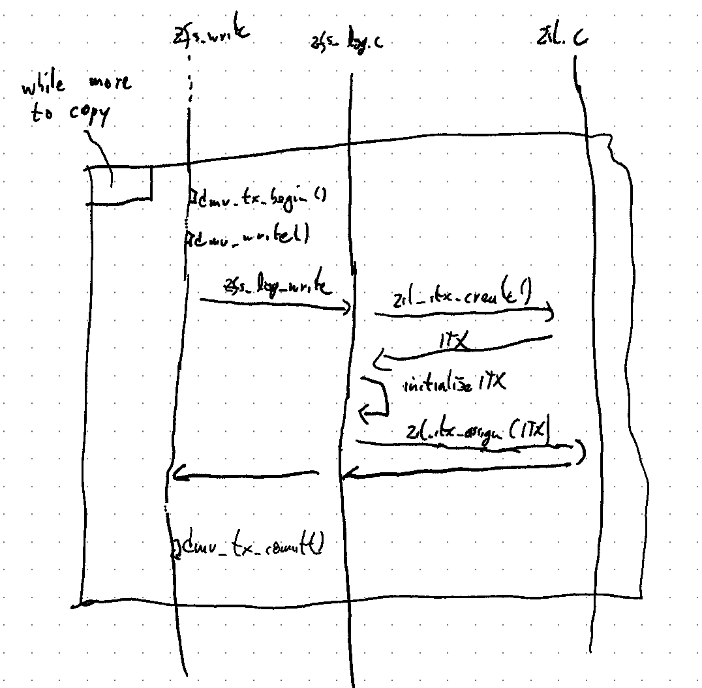
\includegraphics[height=8cm]{fig/zfs_log_write_sequence_diagram}
    \caption{Sequence diagram of the APIs involved in creating the ITXs for a \lstinline{write} system call.}
    \label{fig:zfs_log_write_sequence_diagram}
\end{figure}

\textbf{Alternative \#2}: Since we identified the ZIO pipeline as the main source of latency\todo{ref chapter} in ZIL-LWB, we considered sharing LWBs as a concept between all ZIL kinds.
In that scenario, the ZIL kinds would merely be an alternative to the ZIO pipeline.
A prototype that adopts this approach has been presented at the OpenZFS 2020 Developer summit by \citeauthor{openzfsZILPerformanceImprovements2020}, targeting NVMe drives \cite{openzfsZILPerformanceImprovements2020}
We found this layer of the ZFS software stack to be too restrictive for ZIL-PMEM:
\begin{enumerate}[noitemsep]
    \item The timeout mechanism\todo{ref} for packing multiple entries into a single LWB would add unnecessary latency overhead.
        This is in conflict with one of our requirements (see Section~\ref{sec:requirements}).
    \item This notion is shared by the database community which has deemed group commit schemes --- such as LWB timeout --- unfit for PMEM (see Section~\ref{relw:groupcommit}).
    \item The design space for PRB/HDL would have been severly constrainted.
        In particular, fully parallel logging to the same HDL would not have been possible because the LWB chain is inherently sequential.
        Our ITXG bypass for ZVOLs (see Section~\ref{sec:itxg_bypass}) shows how we can use this feature of PRB/HDL to increase scalability\todo{check,ref} without weakening crash consistency guarantees.
\end{enumerate}

We believe that our design for ZIL kinds introduces ZIL kind specific behavior at a layer that allows for shared crash consistency semantics \textit{and} flexibility in the storage model while minimizing code duplication and thus (hopefully) maintenance cost.
The interface defined by the vtable is a clean abstraction although some design questions (see \ref{sec:zil_kinds:change} and \ref{sec:zil_kinds:suspend_resume}) as well as some LWB-specific APIs (see \ref{sec:zil_kinds:traversal} and \ref{sec:zil_kinds:callbacks}) remain.
The state of each \lstinline{zilog_KIND_t} is truly private do the ZIL kind's implementation.
Neither ZIL-LWB nor ZIL-PMEM access the ITX-related state in the embedded \lstinline{zilog_t} directly, but only through the \lstinline{zilog_t} method that computes the commit list.
If requirements change in the future, the design alternatives presented in the previous section should be considered.

\section{PMEM-aware SPA \& VDEV layer}\label{sec:pmemspavdev}
Prior to the work presented in this thesis, ZFS had no concept of persistent memory.
Fortunately, the requirements of ZIL-PMEM are very limited:
\begin{itemize}[noitemsep]
    \item \texttt{/dev/pmem} SLOGs must be recognized as PMEM SLOG vdevs when they are added to the pool.
    \item The PMEM SLOG's allocatable space must be directly accessible via the PMEM programming model (load/store instructions, cache flushing, \dots).
        If direct access is not possible, the PMEM SLOG vdev must be considered faulty and pool import must be refused.
        We assume that direct access cannot be lost if it is established.\todo{future work: memory hotplug}
\end{itemize}

We add a new boolean attribute \lstinline{is_dax} for \lstinline{disk} VDEVs in the zpool config format.
The attribute indicates whether the VDEV supports direct access through the Liunx Kernel's DAX APIs.
DAX capability is determined by the \lstinline{zpool} command when creating or adding devices to a pool, using \lstinline{libblkid}.
When opening a vdev marked \lstinline{is_dax}, the kernel module ensures that all of the block device's sectors are mappable as one contiguous range of kernel virtual address space.
Failure to establish this mapping fails the onlining process, leaving the vdev in state \lstinline{VDEV_STATE_CANT_OPEN}.
By default, this state prevents the pool from being imported.
If the VDEV is added as a log device, the import process allows the user to specify an override flag, causing the logs to be dropped.\todo{remove that sentence? only confusing}
Note that the \lstinline{is_dax} feature applies to all VDEVs and is independent of ZIL-PMEM.
It merely records the fact that a VDEV is required to be directly accessible via the DAX APIs.
This ensures that future versions of ZFS can leverage DAX capability of main pool VDEVs without needing to change the on-disk format.
Consequently, \lstinline{is_dax} becomes an independent \textit{zpool feature}.

\section{The ZIL-PMEM ZIL Kind}\label{sec:zilpmemzilkind}

\subsection{Activation}\label{sec:zilpmemzilkind:activation}
The ZIL-PMEM ZIL kind is used instead of ZIL-LWB based on the following rule:
\begin{displayquote}
  If the pool has exactly one SLOG and that SLOG is \lstinline{is_dax}, the ZIL kind is ZIL-PMEM. Oterwise, it is ZIL-LWB.
\end{displayquote}
We evaluate this rule during pool import and whenever the pool config changes, i.e.,
\begin{itemize}[noitemsep]
    \item during pool creation,
    \item on \texttt{zpool add} and \texttt{zpool remove}, and
    \item when \texttt{zpool import} is told to drop log devices via the \texttt{-m} flag.
\end{itemize}
To determine whether we need to change ZIL kinds, we compare the resulting desired ZIL kind $k_{desired}$ with the \lstinline{zh_kind} value in any dataset's ZIL header.
If they do not match, we change the ZIL kind as described in Section~\ref{sec:zil_kinds:change}.

The idea behind this approach is to keep administration simple which is a defining paradigm for ZFS~\cite{bonwickZettabyteFileSystem2003}.
From the system administrator's perspective, ZIL-PMEM is automatically used if it supports the user-specified SLOG device configuration, i.e., a single leaf \texttt{/dev/pmem} device.
Otherwise, the system transparently falls back to ZIL-LWB.

Note that this design makes the rule that decides the pool's ZIL kind effectively part of the zpool's on-disk format.
For better maintainablility and forwards-compatibility, the pool's ZIL kind should be encoded in the zpool config instead.

% \subsection{PMEM Space Reservation}

% ZIL-PMEM reserves all of the allocatable space on the PMEM SLOG vdev in order to construct the pool's PRB instance on top of it.
% For this purpose, we prevent metaslab allocation on the PMEM SLOG by placing it into a new allocation class called \lstinline{exempt}.
% We accomplish this by introducing a new allocation class called \textit{exempt} that is never used for block allocation.
% When the user configures a SLOG VDEV that is \lstinline{is_dax}, the \lstinline{zpool} command automatically assigns it to the \lstinline{exempt} class instead of the \lstinline{log} class.
% The allocatable space on the device is thus never used by block allocation and thereby never read or written through ZIO.
% Note that the VDEV labels, which attribute the VDEV to the zpool and store parts of the zpool config, are located outside of the allocatable space.
% Readers and updaters of VDEV labels continue to use block device IO (\lstinline{zio_read_phys} and \lstinline{zio_write_phys}).

% \begin{figure}[H]
%     \centering
%     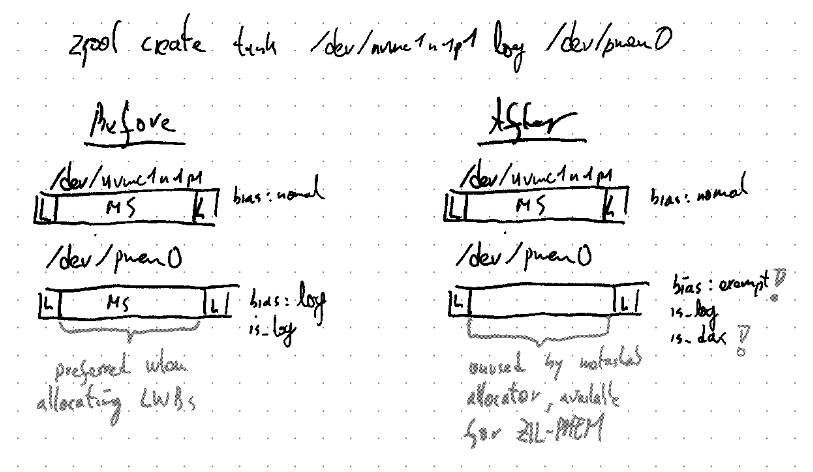
\includegraphics[height=6cm]{fig/pmem_aware_vdev_layer_before_after}
%     \caption{
%         Comparison of the zpool layout before and after the addition of the \lstinline{is_dax} vdev attribute and the \lstinline{exempt} allocation class for PMEM SLOGs.
%     }
% \end{figure}

\subsection{PRB Construction}\label{sec:zilpmem:prbconstruction}
If the pool's ZIL kind is determined to be ZIL-PMEM, ZIL-PMEM uses the entire allocatable space of the (single) PMEM SLOG VDEV to construct the pool's PRB instance on top of it.
The pool import procedure allocates the \lstinline{prb_t} and stores the pointer in the DRAM object that represents the imported pool (\lstinline{spa_t}).
When the pool is exported, the \lstinline{spa_unload} procedure frees the \lstinline{prb_t}.
The \lstinline{prb_t}'s lifetime is thus a contiguous sub-span of the lifetime of \lstinline{spa_t}.

Immediately after allocating the PRB, pool import sets up the chunk objects and adds them to the PRB.
If the pool is being created\todo{correct tense?}, we reset the chunks to a known PMEM state (\lstinline{prb_chunk_initialize_pmem}) before adding them to PRB.\todo{impl is a little different, doesn't matter}
Due to time constraints, our implementation uses a simplistic partitioning scheme that does not need to persist any metadata:
\begin{itemize}[noitemsep]
    \item Chunks have a hard-coded chunk size of \SI{128}{MiB}.
    \item We partition the allocatable space as a contiguous array of PMEM segments of \SI{128}{MiB}, starting at offset zero.
    \item Assuming $A$~bytes of space, this yields \lstinline{nchunks := A>>27} chunks and less than \SI{128}{MiB} of wasted space at the end of the allocated space.
    \item We do not store \lstinline{nchunks} anywhere. Instead, we prohibit online resizing of the PMEM SLOG vdev which allows us to deterministically re-compute the value.
\end{itemize}

\subsection{Dataset \& HDL Lifecycle Synchronization}\label{sec:zilpmem:hdllifecycle}
Whereas \lstinline{prb_t} and \lstinline{spa_t}'s allocation lifecycles line up nicely\todo{language}, the same is not true for datasets and HDLs:
HDLs must be set up during pool import and live until either their dataset destroyed or the zpool is exported.
In contrast, the per-dataset runtime state (\lstinline{dsl_dataset_t}, its \lstinline{objset_t} and the objset's \lstinline{zilog_t}) is allocated \textit{on demand} when its consumer \textit{holds} it by its ID.\todo{don't mention MOS here, we'd need to explain it}
If the consumer is the first holder, the \textit{hold} procedure performs the allocation and recovers state from the corresponding persistent structure (\lstinline{dsl_dataset_phys_t}, \lstinline{objset_phys_t} and, partially, \lstinline{zil_header_t}).
It then increments a reference counter and returns the pointer to the runtime object to the consumer.
Conversely, if there was already another holder, the allocation and recovery steps are skipped.
Once a consumer is finished with a dataset, it \textit{releases} its hold on the DRAM structure.
The last consumer that releases the structure frees the DRAM allocation.

The mismatch of HDL and dataset object lifetimes is relevant to ZIL-PMEM because \lstinline{zilog_pmem_t}\todo{we dropped the name a few times in the ZIL kinds section, ok to use here without explaining?} needs access the corresponding HDL for claiming, replay, and writing log entries.
Our solution is to add a search tree to \lstinline{spa_t} which we call \textit{HDL map}.
It maps from the dataset's object set ID to its HDL.
We add the necessary callbacks to synchronize the \textit{HDL map} with the dataset layer.
%git show ':/make it work (high-level description of what we do in commit msg)'
\begin{itemize}[noitemsep]
    \item During pool import, after setting up the PRB but before claiming, we iterate over the head datasets in the pool, set up the HDLs for each of them, and add them to the \textit{HDL map}.
    \item When a dataset is created (\lstinline{dmu_objset_create_impl_dnstats}), we set up its HDL and add it to \textit{HDL map}.
    \item When a dataset is destroyed (\lstinline{zil_destroy_sync}), we tear down the HDL and remove it from the \textit{HDL map}.
\end{itemize}

Whenever the ZIL-PMEM implementation needs access to th dataset's HDL, it looks up the HDL in the \textit{HDL map} and aquires a reference to it.
We use reference counting to assert that there are no dangling references when the HDL is destroyed in \lstinline{zil_destroy_sync}.
We protect the \textit{HDL map} against concurrent modifications using ZFS's \textit{read mostly lock} which is a reader-writer-lock that is optimized for read locks.
Figure~\ref{fig:zilpmem:datasethdlsync} visualizes the constellation\todo{language} of objects, their lifetimes, and reference relationships.

\begin{figure}[H]
    \centering
    \missingfigure[figheight=7cm]{}
    \caption{The different allocation lifecycles of HDLs and datasets, and how we bridge them for ZIL-PMEM.}
    \label{fig:zilpmem:datasethdlsync}
\end{figure}

\subsection{ZILOG\_PMEM\_T}\label{sec:zilpmem:zilog}
The \lstinline{zilog_pmem_t} structure and its methods in the \lstinline{zilpmem_vtable} implement the ZIL-PMEM ZIL kind.
Its role is that of an adaptor between the shared \textit{itxg} structure that is shared among all ZIL kinds and the HDL that is associated with the dataset via the \textit{HDL map}.
Apart from the exceptions listed below, the methods in the vtable are thin wrappers around HDL's interfaces.
The general pattern for a ZIL-PMEM method is as follows:
\begin{enumerate}[noitemsep]
    \item Aquire a reference to the dataset's HDL from \textit{HDL map}.
    \item Invoke the HDL method.
    \item Release the HDL reference.
\end{enumerate}
To avoid reference counting overhead for HDLs on the write path, we aquire a HDL reference once when the ZIL is opened for writing and hold it in the \lstinline{zilog_pmem_t} until the dataset is unmounted.

The following cases required additional code to adapt betweent he two domains:
\begin{description}
    \item[Error Handling During Pool Import \& Claiming]
        The ZIL vtable was extracted from the original ZIL(-LWB) and inherits its model for integrity checking and claiming of the ZIL during pool import.
        In that phase, ZIL-LWB checks the ZIL chain twice:
        the first pass (\lstinline{zil_check_log_chain}) checks for log corruption to fail the pool import early if the log is corrupt.
        The second pass (\lstinline{zil_claim}) does ZIL-LWB's version of claiming and records the maximum claimed log record in the ZIL header.
        It discards traversal errors because it assumes that no online log corruption happend since the first pass.
        (Note that \lstinline{zil_claim} does have a return value, but only due to software-technical reasons. It must always return zero.)
        ZIL-LWB's approach opens a window for time-of-check vs time-of-use bugs which we discovered and reported during development.\todo{ref}
        In contrast, PRB/HDL does checking and claiming in a single pass (\lstinline{prb_claim}), reports corrupted log state through its return value, and is designed to correctly handle online log corruption during claiming and replay (see Section~\ref{di:prb:ccrecovery}).

        Due to time constraints, we have not refactored the zpool import procedure to allow claiming to fail.
        Until that shortcoming of our implementation is addressed, we trigger a kernel panic if \lstinline{prb_claim} returns an error.

    \item[ZIL Header Updates]
        Remember from Section~\ref{di:prb:api:hdl} on the PRB/HDL API that the responsibility of \textit{persisting} the ZIL-PMEM header is split:
        HDL APIs that update the ZIL header return the updated version through an \textit{out}-parameter and the API consumer is responsible for persisting the update to the main pool.

        Remember also the \lstinline{zil_sync} API from Section~\ref{zilsync}.
        \textit{Txg sync} invokes this method on every dataset's \lstinline{zilog_t} in the \textit{syncing} txg.
        The role of \lstinline{zil_sync} is to modify the dirty copy of the ZIL header that is stored in \lstinline{objset_phys_t::os_zil_header}.
        Unlike most components at this software layer of ZFS, the ZIL implementation itself is responsible for queuing up changes that need to applied for the \textit{open}, \textit{quiescing} and \textit{syncing} txg.

        ZIL-PMEM queues the updated header values returned by the HDL APIs in a 4-ary array that is indexed by \lstinline{[txg&3]}.
        Each cell contains the tuple \lstinline{(txg: u64, header: zil_header_pmem_t)}.
        A header update \lstinline{(txg_u, header_u)} overwrites the cell at index \lstinline{txg_u&3}.
        Updates must only be made from the \textit{open} or \textit{quiescing} txgs.
        \lstinline{zil_sync} then reads cell \lstinline{C := updates[syncing_txg&3]}.
        If \lstinline{C.txg == syncing_txg}, it updates the ZIL header to \lstinline{C.header}.
        Otherwise, it does not modify the ZIL header.

    \item[\lstinline{zil_commit}]
        We implement \lstinline{zil_commit} as follows:
        \begin{enumerate}[noitemsep]
            \item Aquire a \lstinline{zilog_pmem_t}-wide mutex.
            \item Get the \textit{commit list} from the \textit{itxg} data structure.
            \item Invoke the HDL's \lstinline{prb_write_entry} method for each log entry in the commit list, starting a new generation for every entry.
            \item Release the mutex.
        \end{enumerate}
        The mutex ensures that committers are serialized.
        This is critical for the correctness of \textit{sync} or \textit{fsync} which are cummulative.
        Assume two threads $A, B$ that issue the \textit{sync} system call.
        Assume $A$ starts a \textit{sync} system call and drains all ITXs from the \textit{itxg} into its commit list.
        If $A$ is now preempted by $B$ which also starts a \textit{sync} system call, $B$'s commit list will be empty.
        $B$ would return to userspace, giving the caller the impression that all dirty data has been synced, although they still need to be written to the HDL by $A$.

        Starting a new generation for every entry ensures that the commit list's entries will be replayed in commit list order.
        Note that the \lstinline{zilog_pmem_t}-wide mutex already serializes the start of the new generations as required by the HDL API, see Section~\ref{di:prb:api:write}.

        Serializing the entire \lstinline{zil_commit} call allows for less parallelism than ZIL-LWB's \textit{commit ITXs}.
        Commit ITXs implement a sort of\todo{language, help} pipelining by allowing log writers to issue LWB ZIOs in parallel while ensuring that they only return from \lstinline{zil_commit} after all LWBs up to and including the log writer's last LWB have been written.
        Whereas a similar approach cold be applied to ZIL-PMEM in principle by mapping parallel writers to the same generation, the current implementation of \textit{commit ITXs} is too tightly coupled to the concept of LWBs and the ZIO pipeline.

    \item[WR\_NEED\_COPY Chunking]
        Remember from Section~\ref{openzfs:the_zil_api} that the ZIL allocates ITXs for \textit{all} changes to a dataset in DRAM.
        The ITXs are queued in the \textit{itxg} structure from where they are either \lstinline{zil_commit}ted or freed when the txg syncs.
        To avoid unnecessary memory usage and performance overhead, ITXs that log \textit{write} operations do not always contain a copy of the written data.
        Instead, the \lstinline{zfs_log_write} function\todo{ref it, we introduce it in the alternative approach for ZIL kinds section} creates a \lstinline{WR_NEED_COPY} ITX.
        Such ITXs only contain the object number of the DMU object and the range that was modified.
        The creation of the log record is deferred until \lstinline{zil_commit} which reads the range from the DMU object and split it up into many \textit{write} log records.

        For ZIL-PMEM, we implement an isolated structure that turns a single \lstinline{WR_NEED_COPY} record into an iterator over \textit{write} log entries.
        \lstinline{zil_commit} writes each entry yielded by the iterator to the HDL using \lstinline{prb_write_entry}.
        Whereas the repeated chunk aquisition and dependency tracking during each HDL write incurs a small overhead, it also increases fairness among HDLs if the commit slots are contended.

\end{description}

\subsection{ITXG Bypass For ZVOL}\label{sec:itxgbypass}
ZIL kinds are forced into the \textit{commit list} model defined by the shared \textit{itxg} structure which leads to an inherently sequential representation of the ZIL contents:
ZIL-LWB is a long chain of log entries grouped in LWBs, and ZIL-PMEM starts a new generation for every entry on the commit list to encode it properly.
We believe that this architecture is the best compromise for consistent behavior, performance, code duplication, and maintainablility (see Section~\ref{sec:zil_kinds:alternatives}).
Our evaluation in the next chapter shows that ZIL-PMEM yields significant latency benefits and can saturate PMEM bandwidth when performing synchronous I/O from multiple threads to \textit{separate} datasets.
However, the benchmarks show that multi-thread scalability within a \textit{single} dataset is limited.
To demonstrate that PRB/HDL is not the bottleneck, we develop an \textit{itxg bypass} mode for ZIL-PMEM which we present in this section.

\subsubsection{OpenZFS Background: ZVOLs}\label{sec:itxgbypass:openzfsbackground_zvols}
The mode only works for ZVOLs, which are sparsely allocated virtual block devices backed by the zpool.
Other block device consumers, e.g., virtual machines or other file systems, can treat the ZVOL as any other block device exposed by the kernel.
ZVOLs are implemented as a dataset with a single DMU object that contains the virtual block device's data.
When a block device driver accesses the ZVOL block device (\textit{read, write, discard}), ZFS maps the block device operations to DMU operations on the object.
The modifications are logged to the ZIL as ITXs.
If the block device operation has synchronous semantics, ZFS calls \lstinline{zil_commit} before acknowledging completion of the block device operation.
The following pseudo-code describes how the ZVOL processes a block device operation.

\begin{lstlisting}[style=figurepseudocode]
Input:
    op      block device operation
    zv      zvol
Steps:

    if op.pre_flush:
        zil_commit(zv.dmu_object_id)

    match op {
        Read(...) => {
            dmu_read(zv.dmu_object, op.buf, ...)
        },
        Write(...) => {
            tx := dmu_transaction()
            dmu_write(tx, zv.dmu_object_id, ...)
            itx := zil_itx_create(...)
            zil_itx_assign(itx)
            dmu_tx_commit(tx)
        },
        Discard(...) => {
            // analogous
        }
    }

    if op.post_flush:
        zil_commit(zv.dmu_object_id)

    op.done() // acknowledge completion

\end{lstlisting}

The Linux kernel's model for block device I/O is asynchronous.
The assumption is that the block device IO is submitted (\lstinline{submit_bio}), processed asynchronously by the storage device, and eventually marked as completed (\lstinline{BIO_END_BIO}).
By default, ZVOL uses a thread pool (\textit{taskq}s) to process block device I/O asynchronously and in parallel.
The \lstinline{zvol_request_sync=1} tunable changes this behavior to synchronous mode where the procedure outlined above is executed in synchronously in \lstinline{submit_bio}.
We will refer to this tunable in the Section~\ref{todo} where we evaluate the ITXG bypass.

\subsubsection{ITXG Bypass}

In \textit{itxg bypass} mode, we do not queue ITXs in \textit{itxg} but write the log entry/-ies directly to the HDL instead.\todo{language...?}
The role of \lstinline{zil_commit} is reduced to starting a new generation which is necessary to encode a conservative approximation of the logical dependencies between block device operations.
Remember from Section~\ref{di:prb:write:hdlscoped} that the thread that writes the first entry of a new generation must have exclusive access to the HDL.
We use a reader-writer-lock to achieve this behavior, as illustrated by the following pseudo-code.
Note that the actual implementation of the bypass mode is contained within \lstinline{zil_commit} and \lstinline{zil_itx_assign}.

\begin{lstlisting}[style=figurepseudocode]
Input:
    op      block device operation
    zv      zvol
      rwl        reader-writer-lock
      start_gen
Steps:
    if op.pre_flush || op.post_flush:
        zv.rwl.write_lock()
        zv.start_gen = true
    else:
        zv.rwl.read_lock()
        if zv.start_gen:
            zv.rwl.upgrade()

    match op {
        Read(...) => { ... }
        Write(...) => {
            tx := dmu_transaction()
            dmu_write(tx, zv.dmu_object_id, ...)
            itx := zil_itx_create(...)
            prb_write_entry(itx.into_log_entry(), needs_new_gen=zv.start_gen)
            assert zv.start_gen => zv.rwl.holding_write_lock
            if zv.start_gen:
                zv.start_gen = false
            dmu_tx_commit(tx)
        },
        Discard(...) => { /* analogous */ }
    }

    if op.post_flush:
        assert zv.rwl.holding_write_lock
        zv.start_gen = true

    op.done() // acknowledge completion
\end{lstlisting}

\chapter{Evaluation}\label{ch:eval}
In this chapter we evaluate whether ZIL-PMEM meets the project goals established in Section~\ref{sec:requirements}.

\section{Usability \& Architecture}

Our high-level requirements for ZIL-PMEM were: simple administration, sharing of PMEM as a pool-wide resource, same crash consistency guarantees, and coexistence with the existing ZIL(-LWB).
Our design meets all of these requirements:
\begin{description}[noitemsep]
    \item[Simple Administration] Activation of ZIL-PMEM is completely transparent to the administrator.
        There is no change in user experience.
        (See Section~\ref{sec:zilpmemzilkind:activation} for details.)
    \item[Pooled Storage] PRB wraps the PMEM SLOG device and shares it as a pool-wide resource among all HDLs / datasets.
        (See Section~\ref{sec:zilpmem:prbconstruction} for details.)
    \item[Coexistence] The introduction of \textit{ZIL Kinds} allows for coexistence of ZIL-LWB and ZIL-PMEM in code and at runtime.
        The layer at which ZIL kinds were introduced in the architecture allows for sharing of all code that deals with the ZIL's logical structure while providing sufficient freedom to implement a more efficient persistence strategy.
    \item[Same Guarantees] \lstinline{zilog_pmem_t} maintains the same crash consistency guarantees as ZIL-PMEM, courtesy of the shared logical structure and PRB/HDL's guarantees.
\end{description}

\section{Correctness}

We use unit tests and integration tests to validate that our implementation handles expected scenarios correctly.

\subsection{PRB}

We test PRB/HDL's functionality in user space which is possible because PRB/HDL is included in the \textit{libzpool} user-space library.
\textit{libzpool} contains the majority of the ZFS kernel module's code --- it is used to implement \textit{zdb} (the ZFS debugger) and the \textit{ztest} stress testing tool.
We implement our unit tests in Rust to leverage its expressive type and macro system, rich standard library, and its built-in testing harness.
We use the popular \textit{bindgen} crate to generate the bindings to \textit{libzpool} and implement a few idiomatic wrappers to reduce boilerplate code.

\subsubsection{API Walkthrough}
We codify the walkthrough of the PRB/HDL API that we presented in Section~\ref{di:prb:api} in a large test:
\begin{enumerate}
    \item Allocate a ZIL header on the stack.
    \item Create a chunk whose space is allocated from the heap.
    \item Construct PRB and add the chunk to it.
    \item Setup a HDL.
    \item Create a log for the HDL.
    \item Write two entries for $txg=2$ body values $23$ and $42$ to the HDL.
    \item Teardown the object set.
    \item Destroy the PRB with \lstinline{free_chunks=false}. This moves ownership of the chunk moves back from PRB to us.
    \item Construct a new PRB instance with the same chunk.
    \item Setup a HDL from the ZIL header.
    \item Trigger claiming.
    \item Trigger replay, and record the replay callback invocations.
        For each invocation, we read the body length and content, assert that no read error occurred.
        We record body content and the ZIL header update as records in a list.
        We report successful replay for every callback invocation.
    \item After replay is complete, we compare the recorded list's contents to the expected replay order.
\end{enumerate}


\subsection{ZIL-PMEM}

\subsubsection{Correct Handling Of Obsolete Entries}
PRB/HDL assumes that there are only three unsynced txgs at any given time.
This manifests in frequent use of the \lstinline{txg&3} indexing idiom that is common in ZFS.
Whenever state needs to be kept for each of the unsynced txgs, a 4-ary array is used to represent it.
The \lstinline{txg&3}'th element in the array then contains \lstinline{txg}'s state.
The \lstinline{txg} is most often repeated within the per-txg state to detect when an array element is re-used.

In the context of PRB/HDL, it is critical for correctness that an entry $E_i$ for txg $E_i.txg$ is only written if it is either newer than $txg_{open}$ or one of $\{txg_{open}, txg_{open}-1, txg_{open}-2\}$ (dependency tracking, see Section~\ref{di:prb:deptrack}).
We have tests that the \lstinline{prb_write_entry} API does not allow writing entries that do not meet this criterion.
We also cover the replay path and ensure that, if the implementation were incorrect, the replay code would identify the problem with a distinct error code.

\subsubsection{Replay Algorithm}
We structure the PRB/HDL implementation such that it becomes possible to test the core replay logic that we described in Sections~\ref{di:prb:replayapproach},~\ref{di:prb:deptrack},~\ref{di:prb:modeldatacorruption} and ~\ref{di:prb:ccrecovery}:
The idea is to isolate the core logic in a function \lstinline{replay_resume()} that takes as input
\begin{description}[noitemsep]
    \item[NodeSet] the set of entries, represented as \textit{replay nodes}, that were discovered for the HDL,
    \item[ReplayState] a pointer to the DRAM representation of replay state,
    \item[Callback] the callback that receives the \textit{replay node} to be replayed and a pointer to the replay state that needs to be persisted to the ZIL header during replay.
\end{description}
It then constructs the replay sequence from \textit{NodeSet} and invokes the \textit{Callback} for each entry that needs to be replayed, with the replay node and ZIL header update as arguments.
\lstinline{prb_claim()} uses \lstinline{replay_resume()} for ZIL headers in state \textit{logging} to determine $E_{seal}$, and for a dry-run of replay for headers in state \textit{replaying} to detect missing entries early (see Section~\ref{di:prb:ccrecovery}, Step~\ref{ccReplay:claimscan}).
It provides its own \textit{Callback} (\lstinline{prb_claim_cb()}) which only checks that all replay nodes can be read.
\lstinline{prb_replay()} uses \lstinline{replay_resume()} to perform actual for the actual replay.
Its \textit{Callback} (\lstinline{prb_replay_cb()}) serializes \textit{ReplayState} to the representation stored in the ZIL header, builds the ZIL header update, and invokes the user-provided callback.
Figure~\ref{fig:eval:prb_replay_resume_architecture} visualizes this architecture.

\begin{figure}[H]
    \centering
    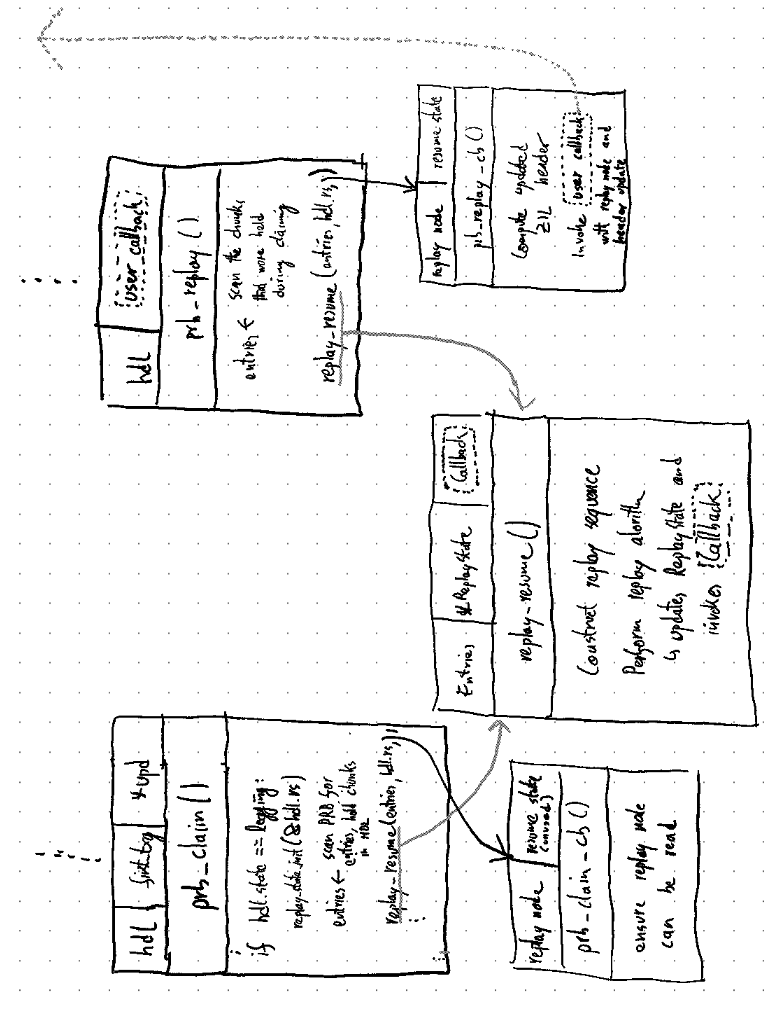
\includegraphics[angle=270,width=\textwidth]{fig/prb_replay_resume_architecture}
    \caption{The architecture that enables code re-use and testability for the core replay logic.}
    \label{fig:eval:prb_replay_resume_architecture}
\end{figure}

\lstinline{replay_resume()} pushes the responsibility to discover entries and to persist replay state to the caller.
This provides maximum flexibility for testing the core logic:
\begin{description}[noitemsep]
    \item[Independence of PRB \& Chunks]
        Testers do not need to mock chunks or parts of PRB that would have to be scanned.
        They also do not need to allocate the actual entries.
        It is sufficient to allocate arbitrary \textit{replay nodes} and to put them into the \textit{EntrySet}
    \item[Independence of ZIL-PMEM]
        It is not necessary to mock or subsititute for any behavior in ZIL-PMEM.
    \item[Crash Consistency Testing]
        To test crash consistency and correctness for resumed replay, the tester can forge an arbitrary replay state in DRAM and invoke \lstinline{replay_resume()} with it.
\end{description}

We leverage Rust's macro system to define test cases in a concise and expressive manner.
Our goal was to minimize the mental step from the two-dimensional grid visualization (See~\ref{fig:prb_hdl_log_structure_example}) to a test case.
The following code snippet is adapted from the test suite.

\begin{lstlisting}
TestSet {
    title: "I- shape",
    entries: maplit::btreemap! {
        // SynthEntry(txg,gen,gsid, (<counters>))
        "A" => SynthEntry(3,10,1, ([(0,0),(0,0),(0,0)])),
        "B" => SynthEntry(4,10,2, ([(0,0),(0,0),(0,0)])),
        "C" => SynthEntry(5,10,3, ([(0,0),(0,0),(0,0)])),
        "D" => SynthEntry(4,11,1, ([(5,1),(4,1),(3,1)]))
    },
    tests: vec![
        test! {
            "tail truncation ok",
            claim_txg = 1,
            // hide entry D during replay and assert that
            // replay does not complain
            stages = stages!(single, hide=&["D"], check=OK,),
            // expected replay callback invocations
            expect_replay = vec!["A", "B", "C"],
        },
        test! {
            "'A missing' detected, but remainder of its gen is replayed",
            claim_txg = 1,
            // hide entry A during replay and ensure that replay
            // complains about missing entries
            stages = stages!(single, hide=&["A"], check=M_ENTRIES,),
            // expected replay callback invocations
            expect_replay = vec!["B", "C"],
        },
    ],
}
\end{lstlisting}

We test the following properties:
\begin{description}[noitemsep]
    \item[Shapes] We test replay for different ``shapes'' in the 2-D grid, e.g., a ``V''-shape with entries for different txgs, or the ``I-'' shape from the snippet above.
    \item[Claim Txg] We ensure that log entries from the $precrash\_txg = claim\_txg - 1$ are ignored during replay.
    \item[Missing Entry Handling] We test the behavior for missing entries in the already replayed and still to be replayed parts of the replay sequence, as well as in the last generation.
    \item[Resumability] We test resumability of \lstinline{replay_resume()} for the cases for the cases of missing entries, re-appearing entries, and no change of \textit{EntrySet} between resume attempts.
    \item[Entry Reappearance] We test that re-appearing entries ordered before the last-replayed entry are ignored, and re-appearing entries in the unreplayed part are discovered and replayed.
\end{description}

\subsubsection{Crash Tests}
We make heavy use of runtime assertions in the implementation to protect against implementation errors.
On the recovery path, almost all assertions are enabled for release builds of the module.
On the write path, most are only enabled for debug builds to improve code generation and runtime performance.
However, \textit{libzpool} is always compiled in debug mode.
We modify \textit{libzpool} such that our test suite can install a hook whenever a runtime assertion triggers.
This allows us to implement \textit{crash tests}
At this time, we use them primarily to ensure that the PRB API triggers assertions if used incorrectly:
\begin{itemize}
    \item Operations on a HDL in the wrong state, e.g., replay of a HDL which was not claimed.
    \item Attempts to set up a HDL that has already been set up.
    \item Writes that exceed the maximum allowed chunk size.
    \item Correct interplay of garbage collection and PRB during PRB allocation (critical for pool export).
\end{itemize}

\subsection{ZIL-PMEM}

Our changes to ZFS are covered (sparsely) by the testing infrastructure of the OpenZFS project.
\begin{description}
    \item[ZFS Test Suite (ZTS)] The ZFS Test Suite is an suite of automated integration tests that asserts behavior of the kernel module and CLI tools.
        ZTS is implemented in Korn shell and consists mostly of functional test.\todo{... of mostly functional tests?}
    \item[ztest] A user-space binary that links against \textit{libzpool} and stress-tests the core components of ZFS that are shared among all support platforms.
        The strategy is to imitate a zpool with lots of concurrent activity initiated from many threads.
        The focus is on code paths in the administrative layer, e.g., dataset creation \& deletion or VDEV management.
        Whereas these code paths are also executed by ZTS, the lack of concurrency in ZTS hides potential race conditions that are discovered using \textit{ztest}.
        \textit{ztest} is designed for easy extensibility.
\end{description}

\subsubsection{ZIL Kinds}
\textit{ztest} has several functions that induce ZIL data path activity (\lstinline{ztest_freeze()})
Whereas these functions use the public ZIL API and required little to no modification, the ztest mocks for datasets (\lstinline{ztest_ds_t}) and its assertions of ZIL state are specific to ZIL-LWB.
Due to time constraints, we
\begin{itemize}[noitemsep]
    \item disabled \lstinline{ztest_freeze()} for ZIL-PMEM and
    \item changed the ZIL-LWB specific assertions to perform a checked downcast of \lstinline{zilog_t} to \lstinline{zilog_pmem_t}.
\end{itemize}.
In the future, this change will need to be reverted and a maintainable design for testing multiple ZIL kinds be devised.
We let \textit{ztest} run once for one hour and did not experience a failure.

\subsubsection{ZIL-PMEM}
After the test run with the ZIL kinds patch, we hard-coded /dev/pmem0 as a SLOG device in \textit{ztest} to get basic testing exposure for ZIL-PMEM.
Despite the disabled \lstinline{ztest_freeze()}, this change helped us discover and fix bugs in the lifecycle of ZIL-PMEM, i.e., dataset creation, mounting, unmounting, and destruction.

Regarding the ZFS test suite, we have identified the following functional tests as relevant for the ZIL and/or SLOG devices:
\todo{proceed with next section}
%% fdfind slog tests
%tests/zfs-tests/tests/functional/slog/slog_{001--015}_*.ksh
%tests/zfs-tests/tests/functional/slog/slog_replay_fs_001.ksh
%tests/zfs-tests/tests/functional/slog/slog_replay_fs_002.ksh
%tests/zfs-tests/tests/functional/slog/slog_replay_volume.ksh
%% fdfind --print0 slog tests  | xargs -0 grep log_assert
%tests/zfs-tests/tests/functional/slog/slog_001_pos.ksh:log_assert "Creating a pool with a log device succeeds."
%tests/zfs-tests/tests/functional/slog/slog_002_pos.ksh:log_assert "Adding a log device to normal pool works."
%tests/zfs-tests/tests/functional/slog/slog_003_pos.ksh:log_assert "Adding an extra log device works."
%tests/zfs-tests/tests/functional/slog/slog_004_pos.ksh:log_assert "Attaching a log device passes."
%tests/zfs-tests/tests/functional/slog/slog_005_pos.ksh:log_assert "Detaching a log device passes."
%tests/zfs-tests/tests/functional/slog/slog_006_pos.ksh:log_assert "Replacing a log device passes."
%tests/zfs-tests/tests/functional/slog/slog_007_pos.ksh:log_assert "Exporting and importing pool with log devices passes."
%tests/zfs-tests/tests/functional/slog/slog_008_neg.ksh:log_assert "A raidz/raidz2 log is not supported."
%tests/zfs-tests/tests/functional/slog/slog_009_neg.ksh:log_assert "A raidz/raidz2 log can not be added to existed pool."
%tests/zfs-tests/tests/functional/slog/slog_010_neg.ksh:log_assert "Slog device can not be replaced with spare device."
%tests/zfs-tests/tests/functional/slog/slog_011_neg.ksh:log_assert "Offline and online a log device passes."
%tests/zfs-tests/tests/functional/slog/slog_012_neg.ksh:log_assert "Pool can survive when one of mirror log device get corrupted."
%tests/zfs-tests/tests/functional/slog/slog_013_pos.ksh:log_assert "Verify slog device can be disk, file, lofi device or any device " \
%tests/zfs-tests/tests/functional/slog/slog_014_pos.ksh:log_assert "log device can survive when one of the pool device get corrupted."
%tests/zfs-tests/tests/functional/slog/slog_replay_fs_001.ksh:log_assert "Replay of intent log succeeds."
%tests/zfs-tests/tests/functional/slog/slog_replay_fs_002.ksh:log_assert "Replay of intent log succeeds."
%tests/zfs-tests/tests/functional/slog/slog_replay_volume.ksh:log_assert "Replay of intent log succeeds."
\begin{description}
    \item[TODO] TODO
\end{description}

The following changes need to be covered by additional ZTS tests:
\begin{itemize}
    \item As described in Section~\ref{sec:zilpmemzilkind:activation}, we plan to automatically activate ZIL-PMEM based on the whether the SLOG device is PMEM.
        However, we have not yet implemented the support for online switching of ZIL kinds for a dataset (Section~\ref{sec:zil_kinds:change}).
        That work should be accompanied by corresponding additions to ztest.
    \item Although we force the replay callback to use the \lstinline{prb_replay_read_replay_node} function which handles \textit{machine check exceptions (MCE)} through \lstinline{memcpy_mcsafe()}, we should somehow ensure that such errors are actually handled.
\end{itemize}

\section{Performance}
We evaluate the performance of ZIL-PMEM using an extensive set of benchmarks.
We seek to answer the following questions:
\begin{itemize}[noitemsep]
    \item What is the speedup that ZIL-PMEM achieves over ZIL-LWB in the 4k synchronous random write workload?
    \item What benefit does ZIL-PMEM provide to applications that frequently perform synchronous I/O?
    \item How does ZFS with ZIL-PMEM perform compared to other Linux filesystems that were adapted to PMEM?
    \item Is ZIL-PMEM a viable alternative to Linux filesystems deployed on top of with dm-writecache?
    \item To what degree do ZVOLs benefit from ZIL-PMEM?
    \item What is the benefit of the ITXG bypass for ZVOLs?
    \item Is PRB's \textit{commit slots} mechanism effective at improving CPU efficiency if the maximum PMEM write bandwidth is exceeded? And what is its overhead?
\end{itemize}

\subsection{Setup \& Methodology}

\subsection{4k Synchronous Random Write Workload}\label{sec:eval:4ksyncwrites}
The first pillar of our performance evaluation is the \textit{fio} 4k synchronous random write workload that motivated the design of ZIL-PMEM.
We already described the workload characteristics in detail in Section~\ref{ch:lwb_analysis:setup}.
We use the same zpool layout as for ZIL-LWB (30 striped NVMe partitions \& 1 non-interleaved Optane DIMM region / \lstinline{fsdax} namespace as SLOG).
We configure PRB with \textit{ncommitters=3}, which is the most CPU-efficient settings for a single Optane DIMM as we will show in Section~\ref{sec:ncommitters_scalability}.

Figure~\ref{fig:eval:fio4k:metrics} shows the cummulative IOPS and per-IOP average latency measured by fio for 1--8 threads.
With a single thread, ZIL-PMEM achieves 128k IOPS which is a speedup of 8 over ZIL-LWB (16k IOPS).
ZIL-PMEM scales almost linearly to 400k IOPS at four threads where the speedup over ZIL-LWB is still $5.5$.
Performance does not increase further for higher thread counts.
The constant offset to the \textit{fsdax} curve for thread count 4--7 suggests that performance is limited by PMEM write bandwidth.
(Remember that \textit{fsdax} shows the raw \texttt{/dev/pmem} block device's performance under the same workload.
The slight decline to 346k IOPS at eight threads correlates with a similar decline in the \textit{async} curve but not the \textit{fsdax} curve, suggesting a CPU bottleneck (8 cores per socket) or scalability bottleneck in ZFS.

\begin{figure}[H]
    \begin{subfigure}{0.5\textwidth}
        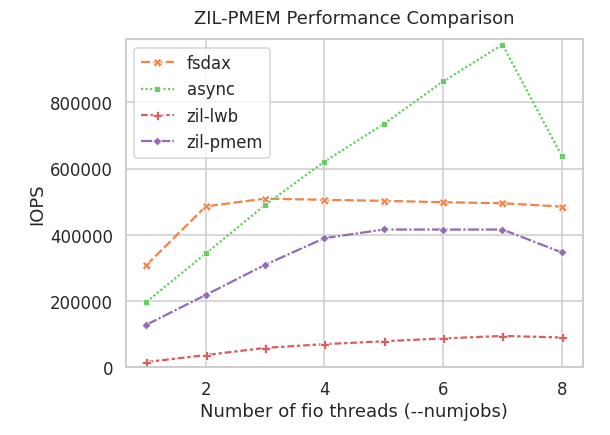
\includegraphics[width=\textwidth]{fig/evaluation/motivating_fio_benchmark__zilpmem__iops}
    \end{subfigure}
    \begin{subfigure}{0.5\textwidth}
        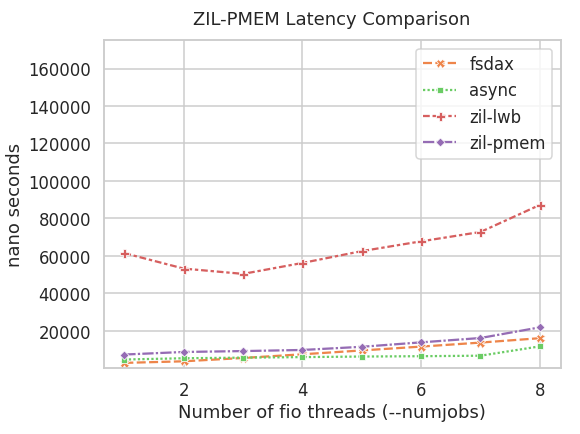
\includegraphics[width=\textwidth]{fig/evaluation/motivating_fio_benchmark__zilpmem__latency}
    \end{subfigure}
    \begin{subfigure}{0.5\textwidth}
        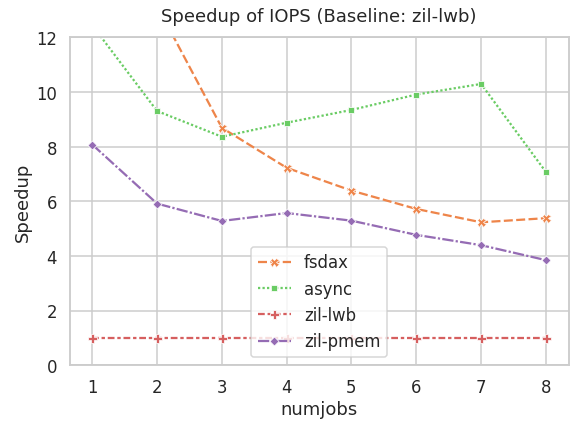
\includegraphics[width=\textwidth]{fig/evaluation/motivating_fio_benchmark__zilpmem__speedup}
    \end{subfigure}
    \begin{subfigure}{0.5\textwidth}
        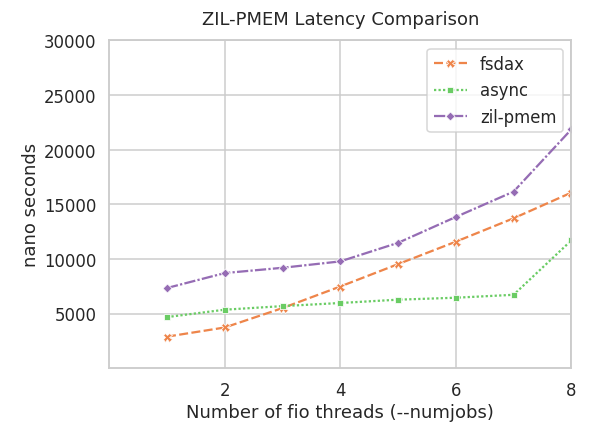
\includegraphics[width=\textwidth]{fig/evaluation/motivating_fio_benchmark__zilpmem__latency_zoomed}
    \end{subfigure}
    \caption{Mean IOPS and latency measured by \textit{fio} for our 4k synchronous random write workload, by number of threads.}
    \label{fig:eval:fio4k:metrics}
\end{figure}

We observed that the speedup for \lstinline{numjobs=1} and \lstinline{2} varies significantly between benchmark runs but remains stable for higher values of \lstinline{numjobs}.
We investigate this issue by computing the coefficient of variation (CoV) of the different configurations based on the mean and standard deviation of IOPS reported by fio.
The results are displayed in Figure~\ref{fig:eval:fio4k:cov}:
The \textit{zil-pmem} CoV remains close to the CoV of \textit{async} until \lstinline{numjobs=4} from where it starts to decline towards the CoV of \textit{fsdax}.
This phenomenon correlates with the stop of increase in IOPS at \lstinline{numjobs=4}, supporting our assumption that \textit{zil-pmem}'s behavior is dominated by the PMEM hardware for numjobs 4--7.
In contrast, \textit{zil-lwb}'s CoV is 5x that of \textit{zil-pmem} for \lstinline{numjobs=1} and 2x for \lstinline{numjobs=2} before it starts to align closely with \textit{async}.
In absolute terms, for \lstinline{numjobs=1}, the standard deviation for ZIL-LWB is 4700 with a mean value of merely 16k IOPS.
In contrast, for ZIL-PMEM, the standard deviation is 7557 at 128k IOPS.

\begin{figure}[H]
    \centering
    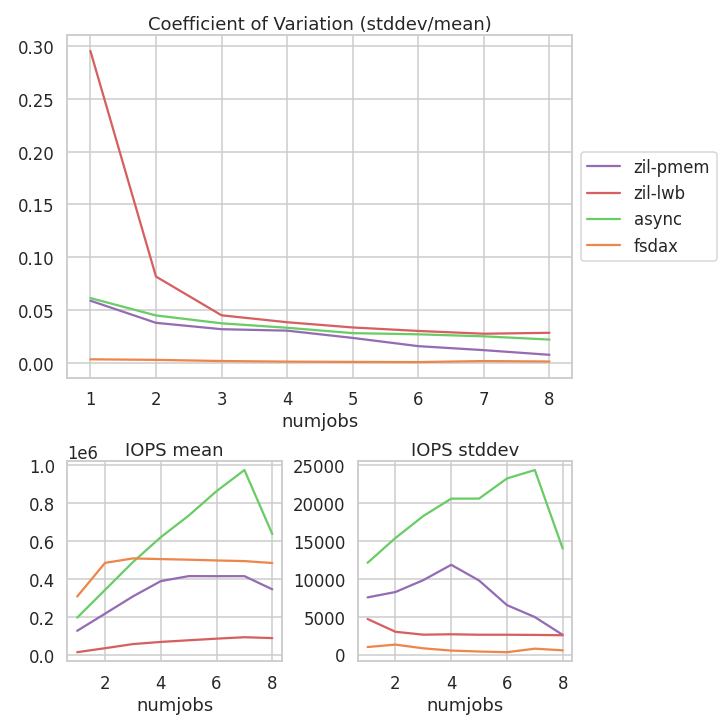
\includegraphics[height=7cm]{fig/evaluation/motivating_fio_benchmark__cov_comparison}
    \caption{Comparison of the coefficient of variation ($\frac{stddev}{mean}$). The smaller plots display the absolute values.}
\end{figure}

To get an idea of ZIL-PMEM's impact on tail latencies, we compare the 5th, 95th, 99.9th, 99.9th, 99.99th and 99.99th's percentiles for completion latency, as reported by fio.
\textit{zil-pmem} follows \textit{async} with a near-constant offset for all percentiles until the expectable knee at \lstinline{numjobs=4}.
\textit{zil-lwb}'s 99.9th and 99.99th percentile show steadier but steeper growth with rising \lstinline{numjobs}.

\begin{figure}[H]
    \centering
    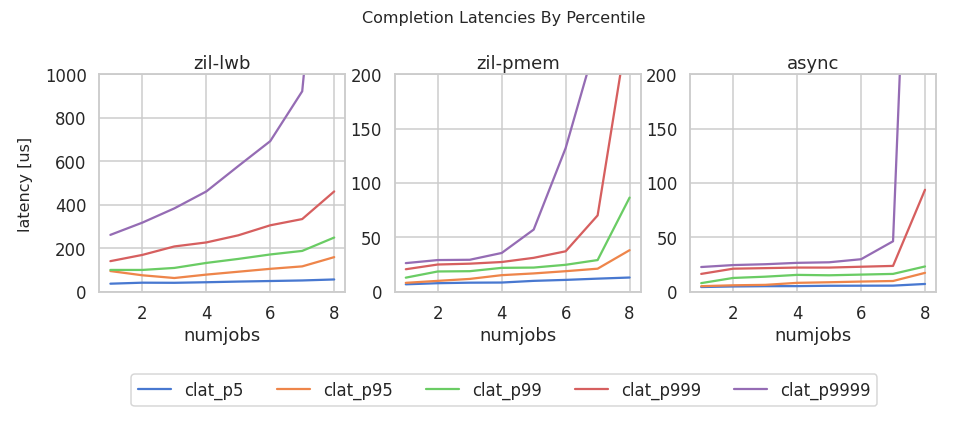
\includegraphics[width=\textwidth]{fig/evaluation/motivating_fio_benchmark__tail_latencies}
    \caption{Comparison of completion latencies by percentile. Note the different y-axis scales.}
\end{figure}

We generalize our eBPF instrumentation from Section~\ref{ch:lwb_analysis:breakdown} to support ZIL-PMEM and compare the resulting breakdown of per-IOP latency in Figure~\ref{fig:eval:fio4k:breakdown}.
The new \lstinline{zil_persistence} component is defined as the overall time spent in \lstinline{zil_commit} minus the time spent filling the commit list.
Whereas it is the dominant factor for latency in ZIL-LWB (80\% of average per-IOP latency, as observed in Section~\ref{ch:lwb_analysis:breakdown}), ZIL-PMEM only spends approximately 25\% on persistence to PMEM.
For ZIL-PMEM, the most dominant component is the \textit{async} code, i.e., modification of DMU objects.
And in contrast to ZIL-LWB, the shared ITX code is a noticable component at 10\% contribution to overall latency.

\begin{figure}[H]
    \centering
    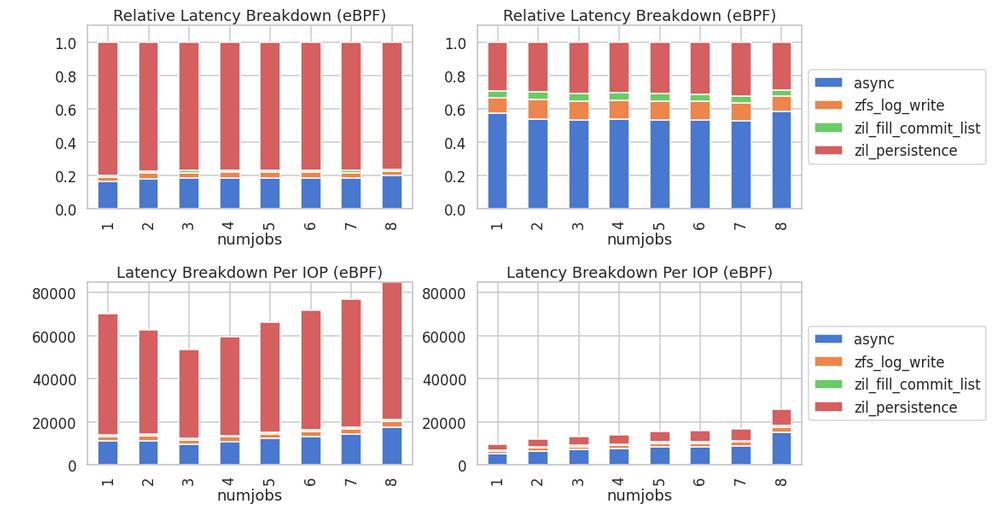
\includegraphics[width=\textwidth]{fig/evaluation/comparison_zil_overhead_lwb_vs_pmem}
    \caption{Comparison of relative and absolute latency contribution of functions executed by fio threads when they perform synchronous writes.}
    \label{fig:eval:fio4k:breakdown}
\end{figure}

\subsection{Application Benchmarks}
We determine ZIL-PMEM's impact on real-world application performance through additional macro-level and application benchmarks.
We execute each benchmarks on top of different \textit{storage stacks} that represent alternatives to ZIL-PMEM and compare the results in the subsequent sections.

We define a \textit{storage stack} as a configuration of storage hardware and software that exposes a filesystem at a mountpoint $M$.
Executing a benchmark \textit{on top of} a storage stack means that the benchmark is configured to place all of its data within the filesystem mounted at $M$.
We define the following storage stacks.
\begin{description}[noitemsep,leftmargin=1.5cm,labelindent=1cm]
    \item[zfs-\{lwb,pmem,sync\_disabled\}] A single ZFS dataset created on a zpool with the familiar hardware configuration (30 striped NVMe partitions and \texttt{/dev/pmem} as SLOG).
        For \textit{zfs-lwb} and \textit{zfs-pmem}, we configure the corresponding ZIL kind.
        For \textit{zfs-sync\_disabled}, we configure the ZIL-LWB ZIL kind but set the \lstinline{sync=disabled} property.
        All variants use a \lstinline{recordsize=4k} and \lstinline{compression=off} on the dataset since most of our benchmarks are synchronous workloads with small write sizes.
        For the \textit{zil-pmem} variant, we configure PRB with \lstinline{ncommitters=3}.
    \item[\{xfs,ext4\}\_\_on\_\_\$BDEV\_\_dax\_\$DAX] Linux 5.9's \textit{xfs} or \textit{ext4} filesystems deployed on the \textit{block device stack} \lstinline{$BDEV}.
        The \lstinline{$DAX} value (\lstinline{True} or \lstinline{False}) indicates whether the \lstinline{dax} mount option was set.
        We always perform benchmark runs without \lstinline{dax}, and perform an additional run if \lstinline{$BDEV} is a DAX-capable device.\todo{make sure DAX is explained}
\end{description}
The \textit{xfs} and \textit{ext4} stacks are parametrized by the \textit{block device stack} \lstinline{$BDEV} which we define as a hardware and software configuration that provides a (potentially virtual) block device.
We define the following block device stacks:
\begin{description}[noitemsep,leftmargin=1.5cm,labelindent=1cm]
    \item[devpmem] The raw \lstinline{fsdax} namespace block device in devfs, i.e., \texttt{/dev/pmem0}.
    \item[dm-writecache]
        The \textit{dm-writecache} Linux Device Mapper target synchro\-nously persists writes to PMEM and performs asynchronous writes-back to an origin block device in the background.
        We configure \textit{dm-writecache} with \texttt{/dev/pmem0} as a cache device and a \textit{dm-stripe} of the 30 NVMe partitions as the origin data store.
        To induce some level writeback, we configure dm-writecache's \textit{low watermark} to 0\% and \textit{high watermark} to 1\%.
        (See Section~\ref{sec:cross_media_storage_systems} for details.)
    \item[zvol-lwb-rs\_\{0,1\}]
        A ZVOL exposed by a zpool in the same config as \textit{zfs-lwb}.
        We set \lstinline{volblocksize=4k} on the ZVOL dataset.
        The \textit{rs} variable controls the value of the \lstinline{zvol_request_sync} tunable which, if enabled, processes block I/O requests (\lstinline{struct bio}) synchronously instead of submitting them to a thread pool.
        (Refer to Section~\ref{sec:itxgbypass:openzfsbackground_zvols} for more details on ZVOLs.)
    \item[zvol-sync\_disabled] Like \textit{zvol-lwb}, but with \lstinline{sync=disabled}.
    \item[zvol-pmem-rs\_\{0,1\}-byp\_\{0,1\}-nc\_3] Like \textit{zvol-lwb}, but configured with the ZIL-PMEM ZIL kind.
        PRB's \lstinline{ncommitters} tunable is always set to $3$.
        The \textit{byp} variable controls whether the ITXG bypass is enabled (0 disabled, 1 enabled).
\end{description}
The following items are examples for storage stacks used in the evaluation:
\begin{description}[noitemsep,leftmargin=1.5cm,labelindent=1cm]
    \item[ext4\_\_on\_\_zvol-pmem-rs\_1-byp\_0-nc\_3\_\_dax\_False] The Ext4 filesystem deployed on a ZVOL on a zpool with the ZIL-PMEM ZIL kind.
        The zpool is configured with \lstinline{zvol_request_sync=1}, disabled ITXG bypass, and \lstinline{ncommitters=3}.
        The ext4 file system is mounted without the \lstinline{dax} mount option.
    \item[xfs\_\_on\_\_devpmem\_\_dax\_True] The XFS filesystem, deployed directly on the PMEM block device (\texttt{/dev/pmem0}).
    It is mounted with the \lstinline{dax} option.
    \item[zfs-pmem] ZFS with the ZIL-PMEM ZIL kind and \lstinline{ncommitters=3}.
        Note that \lstinline{zvol_request_sync} and the ITXG bypass are only relevant for ZVOLs and therefore are not part of the configuration name.
\end{description}

We compare the performance of the storage stacks with the set of benchmarks described below.
To facilitate the comparison, all benchmarks have the following properties:
\begin{description}[noitemsep,leftmargin=1.5cm,labelindent=1cm]
    \item[Scaling factor] The scaling factor increases the degree of concurrent synchronous I/O operations issued by the benchmark.
        We run each benchmark with three scaling factor values: 1, 4, and~8.
    \item[Result Metric] Each benchmark reports a single result metric per run.
        This allows us to compare performance across different storage stacks and scaling factor values.
        For all benchmarks in this evaluation, a numerically greater result metric is better.
\end{description}
What follows is a description of the benchmarks:
\begin{description}[noitemsep,leftmargin=1.5cm,labelindent=1cm]
    \item[fio-growing] The 4k synchronous random write workload that motivated our work, but with all worker thread files within the same filesystem.
        The scaling factor maps to the \lstinline{numjobs} parameter which controls the number of worker threads.
        The working set (amount of modified data) grows with the scaling factor because each additional thread adds a private file with a constant size of \SI{100}{MiB}.
        We report mean IOPS as the result metric.

    \item[fio-fixed] The 4k synchronous random write workload, with all files on a single filesystem, but a fixed working set size, independent of \lstinline{numjobs}.
        We achieve the fixed working set size by setting the \lstinline{size} parameter to $\frac{1~\text{GiB}}{numjobs}$.
        We report mean IOPS as the result metric.

    \item[filebench varmail] Filebench is a benchmarking engine that executes arbitrary workloads described in a domain-specific language.
        The pre-defined \textit{varmail} workload
        ``emulates I/O activity of a simple mail server that stores each e-mail in a separate file (/var/mail/ server).
          The workload consists of a multi-threaded set of create-append-sync, read-append-sync, read and delete operations in a single directory.
          [...] The workload generated is somewhat similar to Postmark but multi-threaded''~\cite{FilebenchGitHubWiki}.
        We use filebench in version \lstinline{1.5-alpha1-33-g22620e6} with the upstream workload definitions.
        The scaling factor maps to the workload's \lstinline{$nthreads} variable which determines the number threads that execute the operations described above.
        We use a runtime of 20 seconds per configuration and report filebench's \textit{ops per second} value as the result metric.

    \item[filebench oltp] The filebench \textit{oltp} workload emulates database workloads.
        It ''performs file system operations using Oracle 9i I/O model.
        It tests the performance of small random reads and writes, and is sensitive to the latency of moderate size (128k+) synchronous writes to the log file.
        By default launches 200 reader processes, 10 processes for asynchronous writing, and a log writer.``~\cite{FilebenchGitHubWiki}.
        We leave all parameters at the default setting except for the \lstinline{$ndbwriters} parameter for which we use the scaling factor's value instead of its default value of ten.
        It is our understanding that scaling the number of log writer threads to a number greater than one would not be feasible with the real DBMS and thus be unrealistic.
        We use a runtime of 20 seconds and report filebench's \textit{ops per second} value as the result metric.

    \item[MariaDB/sysbench] We deploy the MariaDB 10.5.9 Docker image in its default configuration (InnoDB storage engine) with the /var/lib/mysql directory bind-mounted to a sub-directory within the storage stack's mountpoint.
        We apply the \textit{sysbench} benchmark's \textit{oltp\_insert} workload with its default parameters for ten seconds.
        The workload spawns a number of threads that inserts rows with random data into one or more tables.
        We use the default setting (a single table) and map the scaling factor to the number of threads that perform the insert queries.
        Each thread uses a private, long-lived connection to the MariaDB server.
        We use Docker's \lstinline{--net=host} parameter when starting the MariaDB container to allow sysbench to connect via loopback TCP, avoiding the overhead of Docker's user-space proxy.
        The result metric is the number of transactions per second (tps) reported by sysbench.

    \item[Redis-SET] Redis is a popular in-memory key value store.
        For persistence, it provides two mechanisms that are recommended to be used in combination.
        First, the system periodically persists a snapshot of the Redis database (RDB).
        This process happens in the background in a forked child process.
        Second, Redis features a logical write-ahead log (\textit{append-only file}, AOF) that is extended for every mutating operation and replayed after a crash.
        Redis supports three different behaviors for ensuring durability of the AOF, configurable through the \lstinline{appendfsync} configuration variable.
        A value of \lstinline{no} does not perform any fsyncs, \lstinline{everysec} performs an fsync every second (default), and \lstinline{always} performs an fsync operation for operation logged to AOF.
        \cite{RedisPersistenceRedis}

        We deploy Redis 6.2 (built from source).
        We configure RDB writeback to happen every second, regardless of the number of changes,
        We enable AOF and configure \lstinline{appendfsync=always} which effectively turns our Redis deployment into a durable key-value store.

        For benchmarking, we use Redis's own \textit{redis-benchmark} tool~\cite{HowFastRedis}.
        The scaling factor maps to the \lstinline{--threads} and \lstinline{-c} parameters which control the number of parallel clients.
        We use the benchmark's \textit{SET} workload to perform $10^6$ \textit{SET} operations with random keys and the default value size (3 bytes).
        We configure a keyspace size of $10^6$  to reduce contention.
        We leave the values for pipelining and connection keepalive at their defaults (no pipelining, keepalive enabled).
        The result metric is the requests-per-second (rps) value reported by redis-benchmark.

        We choose the number of $10^6$ \textit{SET} operations because it results in runtimes of ten seconds or more for most combinations of scaling factor and storage stacks.
        The only exception is \textit{zfs-sync-disabled} for which the shortes runtime is \SI{8}{s}.

    \item[RocksDB-fillsync] RocksDB is a popular key-value store developed by Facebook that is optimized for fast storage devices.
        It can be used directly by applications as an embedded database but is also the basis for the \textit{MyRocks} storage engine for MySQL~\cite{MyRocksRocksDBStorage}.
        % RocksDB mainline supports PMEM as a LRU cache and several academic publications have proposed deeper PMEM integration.\todo{need to cite it}
        RocksDB uses log-structured merge trees for long-term storage which are written and rewritten in large units that are prepared in DRAM (memtables).
        Operations that request synchronous semantics using the \lstinline{WriteOptions.sync} flag are logged to a write-ahead log file.~\cite{FlushWALLessFwrite,RocksDBGitHubWikiWalPerformance}

        We measure the impact of ZIL-PMEM on RocksDB WAL performance with the \textit{fillsync} benchmark that is part of RocksDB's \textit{db\_bench} tool.
        \textit{Fillsync} performs a fixed number of synchronous \textit{Put} operations with random keys.
        We set the number of operations to 400k and map the scaling factor to the number of concurrently \textit{Put}ting threads.
        The result metric is the \textit{ops-per-sec} (operations per second) value reported by \textit{db\_bench}.

        We choose the number of 400k operations because it results in at least ten seconds of runtime for 90\% of configurations.
        The configurations that achieve less than ten seconds of runtime are:
        \begin{itemize}[noitemsep]
            \item All \textit{zfs-pmem} configurations at scaling factor $1$ ($\sim$\SI{4}{s} runtime)
            \item \textit{zfs-sync-disabled} for scaling factors $1, 4, 8$ (${\sim}2$, $6.8$ and \SI{8}{s} rt.)
            \item \textit{xfs-on-devpmem} with \lstinline{dax} mount option at scaling factor $1$ (\SI{9.1}{s}~rt.)
        \end{itemize}
\end{description}

\subsection{ZIL-PMEM vs. ZIL-LWB}\label{sec:eval:zilpmemvslwb}

\begin{figure}[H]
    \centering
    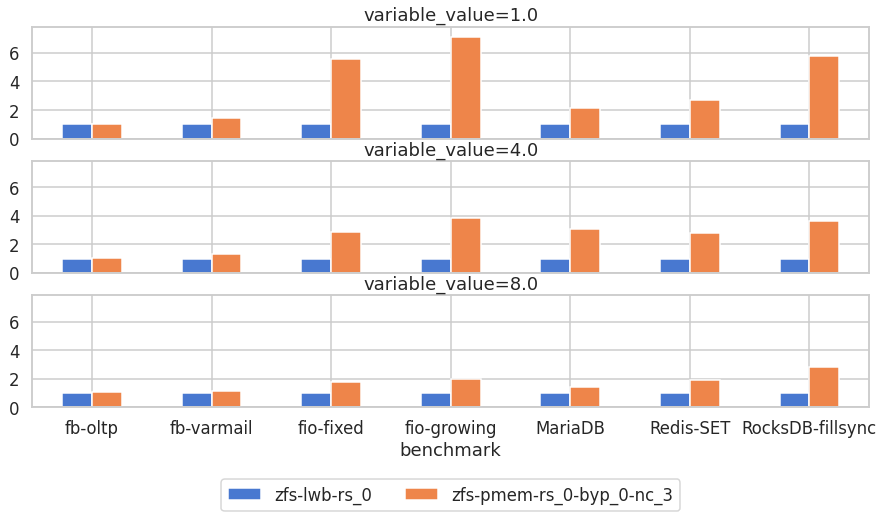
\includegraphics[width=\textwidth]{fig/evaluation/app_benchmarks__zilpmem_vs_zillwb}
    \caption{App Benchmarks: ZIL-PMEM vs. ZIL-LWB with ZIL-LWB as baseline.}
\end{figure}

We first compare the speedup of ZIL-PMEM over ZIL-LWB.
ZIL-PMEM outperforms ZIL-PMEM in all benchmarks, but the speedup varies significantly for the different workloads and scaling factors.
The highest speedups are achieved at scaling factor $1$ by the fio workloads (7.1x, 5.3x) and \textit{RocksDB-fillsync} (100k ops-per-sec, a speedup of 5.8).
\textit{Redis-SET} achieves shows a speedup of $2.68$ (30k rps) and MariaDB achieves 10k tps which is a speedup of 2.14.
For scaling factor $4$, the fio and RocksDB's speedup declines whereas Redis's grows to 2.77 and MariaDB's grows to 3.08.
For scaling factor $8$, all workloads show a reduction in speedup (RocksDB 2.8x, Redis 1.9x, MariaDB 1.4x).

The \textit{filebench-oltp} workload shows no relevant speedup or slowdown for all scaling factor values.
We observed during benchmark execution that the 200 reader processes always cause 100\% CPU utilization.

The \textit{filebench-varmail} workload only shows a speedup of $1.4$ at scaling factor 1 which shrinks to $1.1$ at scaling factor 8.
A possible explanation for these meager results is the larger data volume (16k appends) compared to the fio workloads (4k writes).
In combination with the large amount of metadata (file creation and deletion), ZIL-LWB might also be benefitting from the \textit{commit ITXs'} pipelininig.
In any way, \textit{filebench-varmail} shows that the large speedups for small writes cannot be generalized to all filesystem workloads.
Future work should investigate ZIL-PMEM's behavior during this benchmark in detail and determine how beneficial pipelining akin to \textit{commit ITXs} could be.

\subsection{ZIL-PMEM vs. XFS and Ext4 on PMEM}

Our next set of results is the comparison between ZFS and the Linux filesystems XFS and Ext4.
We include both ZIL kinds (\textit{lwb}, \textit{pmem}) as well as \lstinline{sync=disabled} to demonstrate the upper bound for any ZIL kind.
Both XFS and Ext4 are DAX-aware and thus we inlcude configurations with and without the \textit{dax} mount option.
%Note that, since the ZIL unconditionally journals all data, including file contents, the \textit{lwb} and \textit{pmem} ZFS configurations provide significantly stronger crash consistency guarantees than the Linux filesystems which only journal metadata.
%Nope, that argument is moot because all workloads use fsync and all the filesystems impmlement it correctly (hopefully).
Note that that the ZFS configurations only use PMEM for the ZIL but NVMe devices for permanent storage whereas the Linux filesystem configurations are PMEM-only.

\begin{figure}[H]
    \centering
    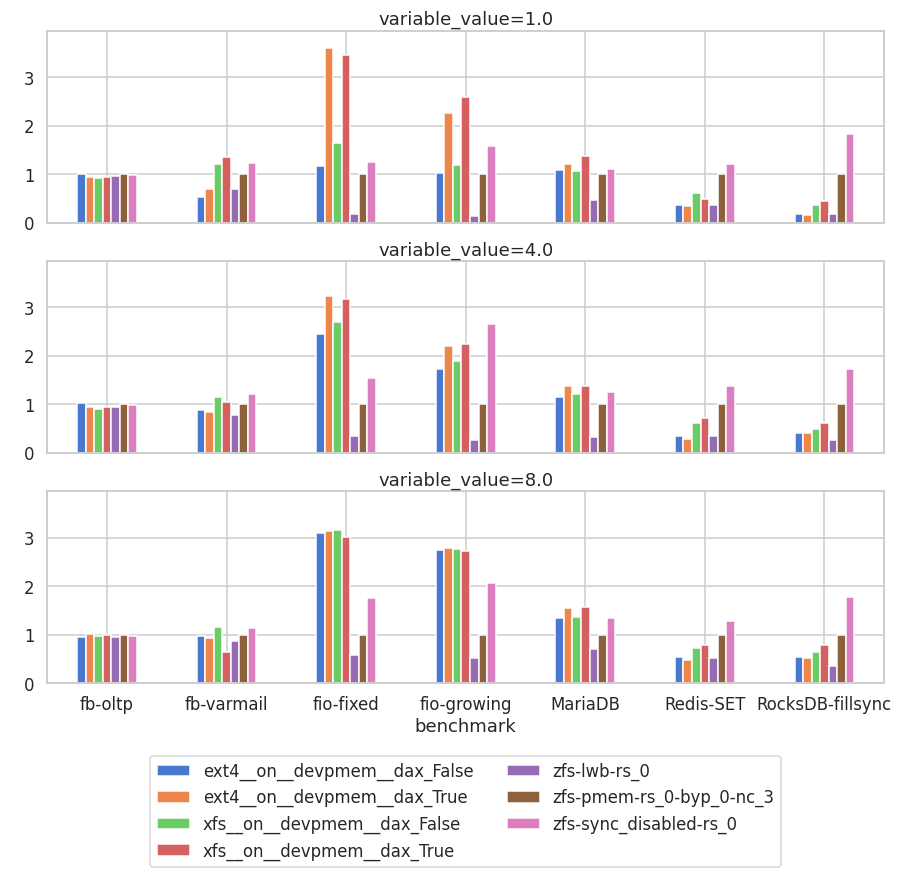
\includegraphics[width=\textwidth]{fig/evaluation/app_benchmarks__filesystems}
    \caption{
        Speedups of ZFS with ZIL-LWB and \lstinline{sync=disabled} as well as ext4 and xfs with and without the \textit{dax} mount option over ZIL-PMEM as baseline.
    }
\end{figure}

Our primary takeaway from this comparison is that, in contrast to ZIL-LWB, ZIL-PMEM is competitive with both ext4 and xfs at scaling factor $1$ in most benchmarks.
The fio workloads are the exception, where the Linux filesystems achieve a speedup of greater than $3$ if the \textit{dax} mount option is enabled.

ZIL-PMEM performs significantly better than all other configurations (excluding \lstinline{sync=disabled}) for \textit{Redis-SET} and \textit{RocksDB-fillsync} at all scaling factors.
The write-ahead log files written by these workloads are append-only and contain the encoded representation of logical changes.
The mutating requests issued by our benchmarks have small payloads and result in small \lstinline{write+fsync} system calls.%
\footnote{
    The RocksDB documentation and comments in the source code suggest that the WAL files are written in 32k blocks that are zero-padded if necessary~\cite[db/log\_writer.h]{RocksDBGitHubWikiWalPerformance}.
    We observed the contrary behavior with \lstinline{strace}: each \textit{Put} operation with \lstinline{WriteOptions.sync} results in a \lstinline{write} and \lstinline{fdatasync} system call. The \lstinline{write} system call's data size is proportional to the sum of the \textit{Put} operation's key and value sizes.
}
ZIL-PMEM handles this workload more efficiently than the Linux filesystems because the ZIL's data journaling causes less write amplification than the Linux filesystems whose latency is likely dominated by page-granular write-back on every \lstinline{fsync}.

In the \textit{MariaDB} benchmark, the DAX-aware Linux filesystem configurations achieve up to 1.6x more transactions per second than ZIL-PMEM.
The \lstinline{sync=disabled} workload is on-par with the non-DAX-aware configurations, at speedups over ZIL-PMEM of ca. 1.1, 1.2 and 1.3 at scaling factors 1, 4, and 8.
Manual inspection of the CPU utilization shows a signficant amount of context switching but no clearly identifiable CPU bottleneck.
% strace -e pwrite64,fdatasync -f -p $(pgrep mysqld)     
% ls -lah /proc/$(pgrep mysqld)/fd                       
% => mostly 1024B writes to ib_logfile0 which according to https://mariadb.com/kb/en/innodb-redo-log/ is the redo log file
The database server process performs 1024 \lstinline{write} + \lstinline{fdatasync} system calls to the InnoDB redo log file from a single thread.
However, since \lstinline{sync=disabled} does not perform better than any of the systems that actually write to PMEM, we can also rule out a PMEM bandwidth as a possible bottleneck.
\todo{need to state that we do not have a final conclusion here?}

Regarding the \textit{filebench-oltp} benchmark, no configuration performs exceptionally better than any other, including \lstinline{sync=disabled}.
We observe high CPU utilization in all benchmark configurations, caused by the \textit{hog} stage of the 200 processes that simulate reader threads.
Thus, CPU is most likely the bottleneck in all configurations.

For \textit{filebench-varmail}, the highest speedup is 1.35 at scaling factor $1$, achieved by XFS in DAX-aware mode, followed by ZFS with \lstinline{sync=disabled} with 1.22x.
For higher scaling factors, the speedups are slightly lower.
The fact that \lstinline{sync=disabled} achieves a lower speedup than XFS can be taken as an indicator that \textit{filebench-varmail} is not bound by PMEM performance, contradicting our speculation in the previous section.

\subsection{ZIL-PMEM vs. XFS and Ext4 on Dm-writecache}\label{sec:eval:dmwritecache}

A fairer comparison is thus the deployment of the Linux filesystems on top of \textit{dm-writecache} with a \textit{dm-stripe} of the NVMe partitions as the origin block device.
The comparison betwen ZIL-PMEM with NVMe storage and Linux filesystems on pure PMEM in the previous section is insightful but not a level comparison.
The ZFS configuration only uses PMEM as short-term storage to bridge the gap between the background txg syncs to the striped pool of NVMe partitions.
%And while we disable ZFS's advanced features such as encryption, redundancy, compression, and deduplication for our benchmark, they are readily available.
In contrast, the Linux filesystem configurations store all their data on PMEM.
Essentially, this 

\begin{figure}[H]
    \centering
    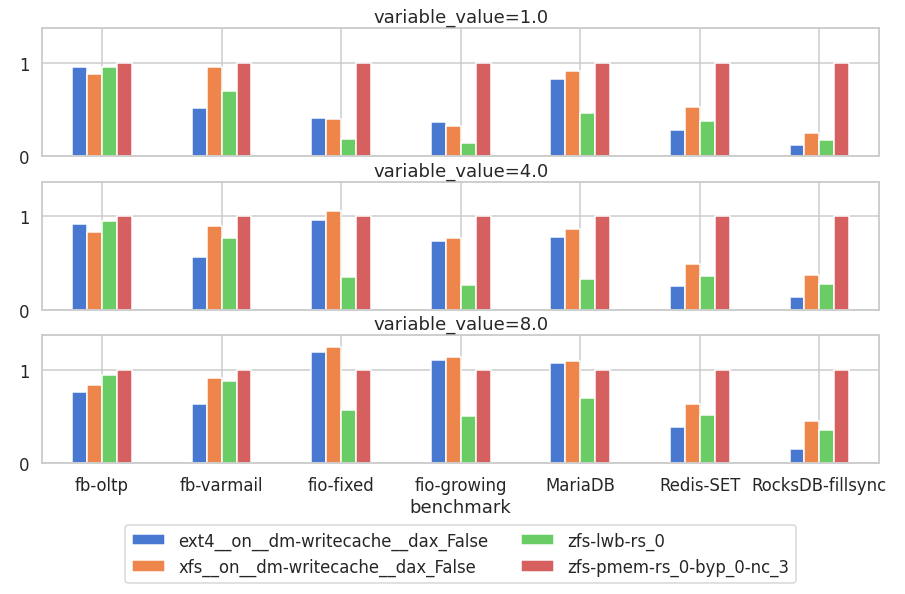
\includegraphics[width=\textwidth]{fig/evaluation/app_benchmarks__dm-writecache.png}
    \caption{
        Comparison of Linux filesystems on dm-writecache with ZIL-PMEM as a baseline.
    }
\end{figure}

ZIL-PMEM's performance is within +/-30\% of XFS on \textit{dm-writecache} at all scaling factors in all benchmarks except \textit{Redis-SET} and \textit{rocksdb-fillsync} where ZIL-PMEM performs significantly better.
The 30\% spread decreases slightly with higher scaling factor but does not change the overall impression\todo{better word?}.
Our explanation for ZIL-PMEM's significantly better performance in the \textit{Redis-SET} and \textit{rocksdb-fillsync} workloads is (again) write amplification:
due to ZFS's integrated design (filesystem and volume manager), the ZIL is able to write logical changes directly to PMEM with little write amplification.
In contrast, dm-writecache hides PMEM behind the block device interface, prohibiting direct access to PMEM (i.e., the \textit{dax} mount option is not avaialble).

Ext4 performs signficantly worse than ZIL-PMEM (and XFS!) in some benchmarks, with only 45\%, 28\%, and 14\% of ZIL-PMEM's performance in \textit{filebench-varmail}, \textit{Redis-SET}, and \textit{rocksdb-fillsync} at scaling factor~1.
Write amplification might be a possible explanation as well.

We have manually observed the system while benchmarking the \textit{dm-writecache} stack to ensure that the comparison with ZFS is actually fair.
We found that, despite the very aggressive write-back configuration (high watermark = 1, low watermark = 0), the system performed very little write-back to the NVMe drives.
The two \textit{fio} workloads were the exception but the write load towards the NVMe devices was well below their maximum capacity.
Thus, NVMe was not a bottleneck in the benchmark.
However, we found that \textit{dm-writecache} has severe multi-core scalability problems.
For example, XFS on raw PMEM without the \textit{dax} mount option achieves 150k IOPS at scaling factor 1 and 409k IOPS at scaling factor 4.
In contrast, on dm-writecache, it is 112k IOPS at scaling factor 1 but only 165k IOPS at scaling facto 4.
Using the \textit{perf} tool, we observed severe contention at a lock that serializes access to the entire dm-writecache instance's state.
In private communication, dm-writecache's maintainer Mikulas Patocka stated that "the purpose of dm-writecache is to decrease commit latency, not to increase throughput. There is not much that can be done with the lock contention".\todo{waiting for permission to quote him publicly}
ZIL-PMEM has similar problems (125k at factor 1, 217k at factor 4) albeit due to the sequential structure of ZIL chain.
In the next section, we show how a more relaxed log structure such as the ITXG bypass can improve the situation.\todo{is this a good transition?}

\subsection{Impact on ZVOL Performance \& ITXG Bypass}

In this section, we examine the impact of ZIL-PMEM on ZVOL performance.
We compare the performance of XFS deployed on a ZVOL in a zpool with varying ZIL kinds, \lstinline{zvol_request_sync} (\lstinline{rs_{0,1}), and ITXG bypass setting (\lstinline{byp_{0,1}).
The results are relative to \textit{zvol-pmem-rs\_0-byp\_0-nc\_3} as the baseline which is the standard configuration for ZIL-PMEM pools.
Note that deploying a filesystem on a ZVOL generally makes little sense in practice because ZFS filesystems provide the same basic service with more additional features at less overhead.
However, ZVOLs are a popular choice for storage virtualization where ZVOLs are used as virtual hard disks, either on the same host or via a SAN (e.g., iSCSI, Fibre Channel).
To simplify our evaluation, we avoid the overhead of a hypervisor or SAN and instead instantiate XFS directly on top of the ZVOL, mount it, and execute the benchmarks.

\begin{figure}[H]
    \centering
    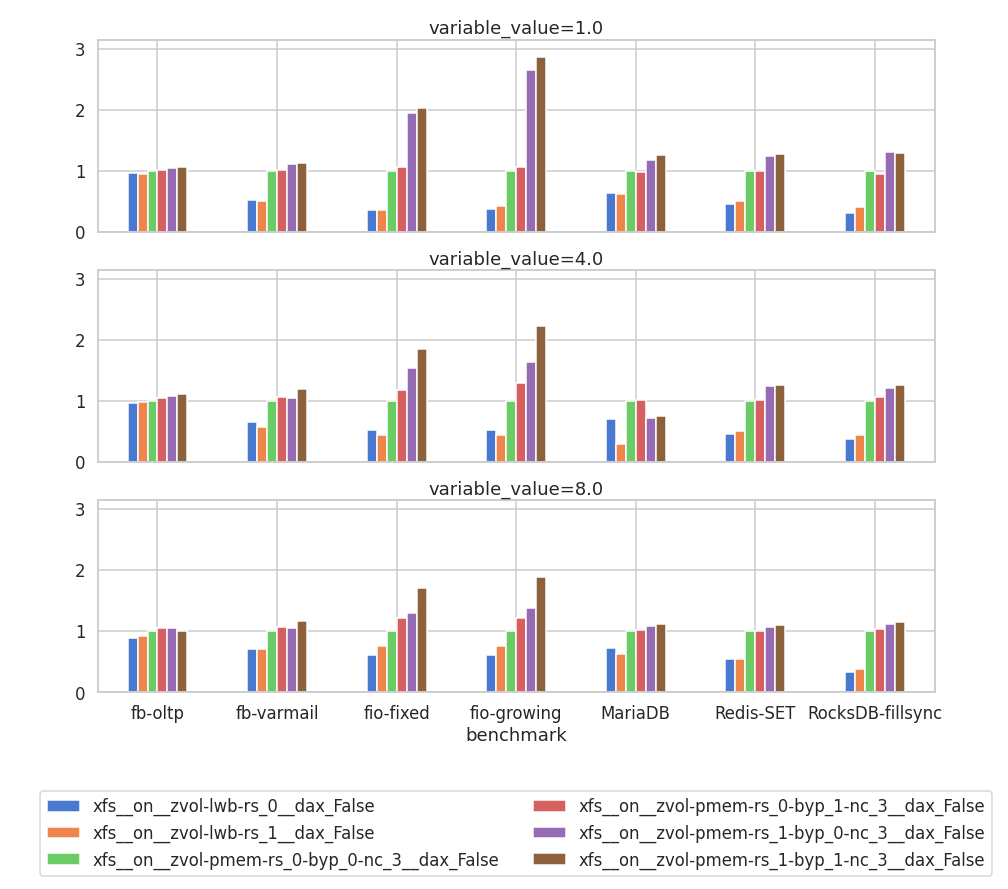
\includegraphics[width=\textwidth]{fig/evaluation/app_benchmarks__zvol_xfs}
    \caption{
        Comparison of XFS on ZVOLs on different zpool configurations.
    }
\end{figure}


ZIL-PMEM in its default configuration delivers a significant speedup over ZIL-LWB.
At scaling factor 1, it is approximately 2x for all workloads except \textit{MariaDB} ($\frac{1}{0.68} = 1.47$) and \textit{filebench-oltp} ($\frac{1}{0.96} = 1.04$).
At higher scaling factors, the speedup declines for all benchmarks albeit less so with \textit{Redis-SET} and \textit{RocksDB-fillsync} than with the other workloads.

The effect of \lstinline{zvol_request_sync=1} is ambiguous and not very signficant for ZIL-LWB but very beneficial for ZIL-PMEM in the \textit{fio} workloads at scaling factor 1 with a 2x and 2.6x speedups over the standard configuration, respectively.
\textit{MariaDB}, \textit{Redis-Set} and \textit{RocksDB-fillsync} also benefit with speedups of 1.18x, 1.23x, and 1.30x.
However, for scaling factor 4, \textit{MariaDB} performs substantially worse if \lstinline{zvol_request_sync} is set (30k tps vs. 20k tps).
We also conducted the benchmarks with Ext4 instead of XFS (not shown in the plot).
Ext4 exhibited worse performance in almost all configurations if \lstinline{zvol_request_sync} was set, with the exception of the \textit{fio} workloads.

The ITXG bypass only has marginal effects with and without \lstinline{zvol_request_sync}, except for the \textit{fio} workloads at scaling factors 1 and 4.
For example, \textit{fio-growing} at scaling factor 8 shows an increase in IOPS from 84k to 102k (21\%) for \lstinline{zvol_request_sync=0} and from 117k to 159k (35\%) with \lstinline{zvol_request_sync=1}.
For Ext4, \textit{filebench-varmail} also shows a 20\% improvement with enabled ITXG bypass and \lstinline{zvol_request_sync=0}.
Activation of the ITXG bypass does not appear to have a negative impact for XFS in the remaining workloads.
For Ext4, we observed some performance degradatations in setups whether both ITXG bypass and \lstinline{zvol_request_sync} were enabled.

In summary, ZIL-PMEM provides a signficant performance advantage for ZVOLs but is less effective than than with ZFS filesystems (see Sections~\ref{sec:eval:4ksyncwrites} and \ref{sec:eval:zilpmemvslwb}).
This is particularly noticable for the \textit{fio} workloads and \textit{RocksDB-fillsync}.
Their speedup with ZIL-PMEM on XFS+ZVOL is only half the speedup of what we observed for ZFS at scaling factor~1.
Write amplification cannot be responsible for this behavior because only \textit{RocksDB-fillsync} causes write amplification.
The most likely cause is latency overhead added by the filesystem that affects all workloads equally.

\subsection{CPU-Efficient Handling Of PMEM Bandwidth Limits}\label{sec:ncommitters_scalability}

PRB's \textit{commit slot} mechanism limits the amount of parallel writers to PMEM through the \lstinline{ncommitters} variable.
The goal is to avoid wasteful on-CPU stall cycles which inevitably occur if the aggregate write bandwidth to PMEM exceeds the hardware capacity.
(See Sections~\ref{sec:requirements} and \ref{di:prb:write} for a more detailed explanation.)

To determine the mechanism's effectiveness, we use our 4k synchronous random write workload with separate ZFS filesystems per fio thread.
We add low-overhead per-CPU counters to ZIL-PMEM to sum up the total mount of time that is spent writing PMEM ($T_{pmem}$), as well as the number of write operations performed during the benchmark ($N_{ops}$).
We then compute the \textit{average PMEM write time per IOP} $T_{pmem_{iop}} = \frac{T_{pmem}}{N_{ops}} [\frac{s}{op}]$.
The most efficient value for \lstinline{ncommitters} for a given system then depends on the workload and efficiency goals.
In general, \lstinline{ncommitters} should be the minimal value where $T_{pmem_{iops}}$ is tolerable but the system's primary performance metric is not impacted.

We compute $T_{pmem_{iops}}$ for 1 to 18 numjobs, different values of \lstinline{ncommitters} and two different PMEM configurations.
The first PMEM configuration is a single, non-interleaved Optane DIMM.
The second configuration are four interleaved Optane DIMMs.
Regardless of how interleaving is configured, we create a \SI{40}{GiB}-sized \textit{fsdax} namespace on the resulting region and use it as the PMEM SLOG for ZIL-PMEM.
We use a machine with higher core count for the benchmarks.
The system configuration is as follows:
\begin{description}[noitemsep,leftmargin=1.5cm,labelindent=1cm]
    \item[System] Supermicro SYS-1029U-TRT
    \item[Mainboard] Supermicro X11DPU, Version 1.10
    \item[CPU] 2 x Intel(R) Xeon(R) Gold 5220 CPU \@ 2.20GHz \\
        18 cores per socket, 2-way SMT per core
    \item[DRAM] 12 x 32GiB SK HYNIX DDR4-2666, HMA84GR7CJR4N-VK  % sudo dmidecode | grep -C8 DRAM | grep 'Part Number'
    \item[PMEM] 8 x Intel Optane DC Persistent Memory, 128 GB, (NMA1XXD128GPS), 4 per socket.
    \item[NVMe] System rootfs only, no dedicated NVMe hardware.
    \item[Kernel] Linux Kernel, Fedora 5.11.15-100.fc32.x86\_64
    \item[Userland] Fedora 32
    \item[fio] fio-3.21
\end{description}
As with our main evaluation system (described in Section~\ref{ch:lwb_analysis:setup}), we leave SMT enabled.
We disable the second socket in software using the \lstinline{isolcpus=18-35,54-71} kernel command line parameter.
Since the system does not have NVMe devices available, we provision the disabled socket's Optane DIMMs in \lstinline{AppDirectNotInterleaved} mode with one PMEM region and a single \lstinline{fsdax} namespace per DIMM.
We use these namespaces as the zpool's main (non-SLOG) vdevs.
% NOTE: we use \lstinline / ttt for ncommitters and math-mode for numjobs. 

\begin{figure}
    \centering
    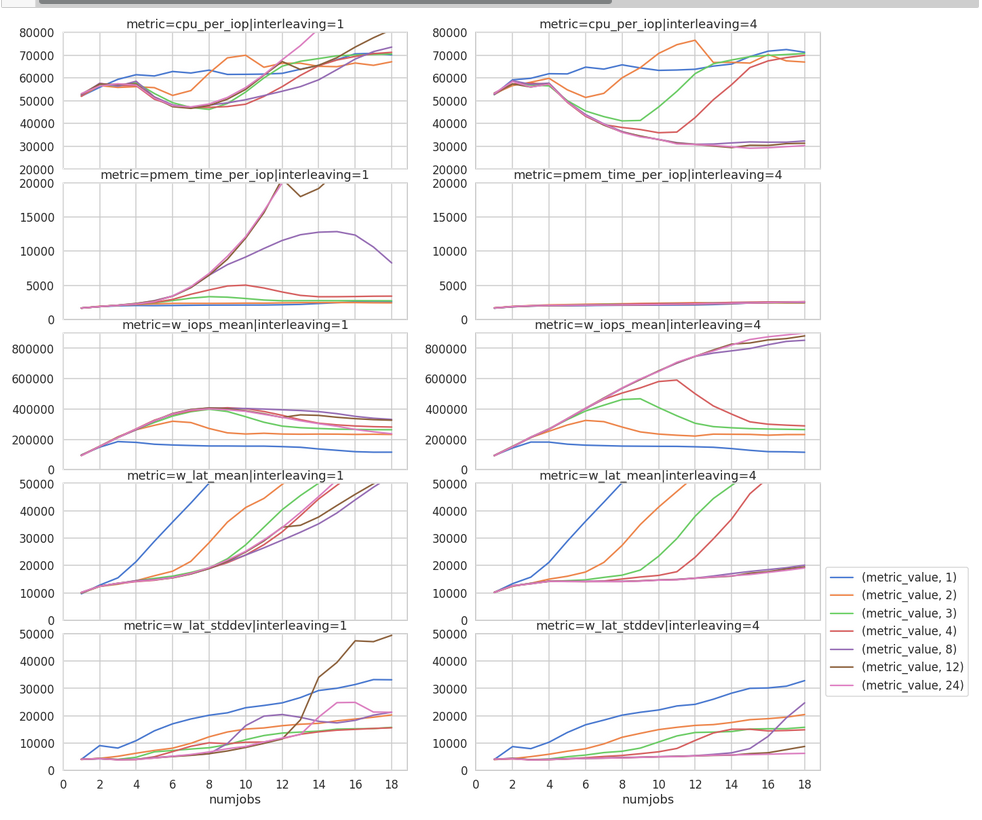
\includegraphics[width=\textwidth]{fig/evaluation/ncommitters_scalability__comparison}
    \caption{Comparison of performance and PMEM write time per IOPS for different values of \lstinline{ncommitters} in two PMEM configurations (left non-interleaved, right four-way interleaved).}
    \label{fig:eval:ncommitters_scalability:main}
\end{figure}


Figure~\ref{fig:eval:ncommitters_scalability:main} visualizes the results of this experiment.
For the non-interleaved configuration, we observe that the system's peak IOPS is 400k, first achieved with \lstinline{ncommitters=3}.
For \lstinline{ncommitters=3}, IOPS quickly decline to 263k IOPS for higher $numjobs$.
With \lstinline{ncommitters=8}, the system is able to sustain the 400k IOPs for the for $numjobs \in 7 \dots 13$.
The price is significantly more on-CPU PMEM time per IOP:
looking at $numjobs = 8$, the $T_{pmem_{iops}}$ is $3300, 4300, 6500~\text{ns}$ for \lstinline{ncommitters=3, 4} and \lstinline{8}.
And at $numjobs = 12$, $T_{pmem_{iops}}$ climbs to $11600, 20600~\text{ns}$ for \lstinline{ncommitters=8} and \lstinline{12} whereas \lstinline{ncommitters=3} is successfully limited to $2700~\text{ns}$ of PMEM write time per IOP.
The \lstinline{ncommitters=12} and \lstinline{24} configurations do not achieve higher peak IOPS than \lstinline{ncommitters=8} but decline to lower values for high $numjobs$, e.g., only 237k IOPS for \lstinline{$ncommitters=24}, $numjobs = 18$.
This performance decline at high degrees of concurrency is a property of the Intel Optane PMEM hardware~\cite{yangEmpiricalGuideBehavior2020}.
The limitation to \lstinline{ncommitters=8} mitigates this effect (331k vs. 237k IOPS at $numjobs = 18$).

The four-way interleaved configuration exhibits a very different behavior.
We achieve the highest IOPS for the configuration where the \textit{commit slot} mechanism has no effect, i.e., \lstinline{ncommitters=24}, $numjobs = 18$ with 900k IOPS.
Given that the IOPS curve has not reached a plateau at this point, a higher value might be possible with higher $numjobs$.
$T_{pmem_{iops}}$ is the same for all \lstinline{ncommitters} values at a given $numjobs$ value (+/- $100~\text{ns}$).
It is $1660~\text{ns}$ for $numjobs = 1$ and grows slightly unevenly towards $2560~\text{ns}$ at $numjobs = 24$.
This is an increase of merely 54\% which is likely to be acceptable in any setup, given the 9.6x increase in IOPS (93k to 900k) that is possible with \lstinline{ncommitters=24}.

To determine the \textit{commit slot} abstraction's impacts performance in ${\footnotesize\texttt{ncommitters}} > numjobs$ configurations, we add additional instrumentation that measures the average latency of commit slot aquisition and release.
Figure~\ref{fig:eval:ncommitters_scalability:overhead} visualizes the results for \lstinline{ncommitters=24}.
The absolute overhead is approximately the same for both PMEM comfigurations.
It starts at $100~\text{ns}$ for $numjobs = 1$, climbs to $240~\text{ns}$ at $numjobs = 4$, and then scales linearly to $385~\text{ns}$ at $numjobs = 18$.
In the interleaved configuration, for any $numjobs > 4$, this corresponds to approximately 11--13\% of the overall write latency per log entry.
Without \textit{commit slots}, \lstinline{zil_commit} could thus be $\frac{1}{1 - 0.13} = 14.9\%$ faster.
However, due to the overhead of the other ZFS components, the contribution to overall IOP latency is only 2\%, which would constitute a rather meager improvement.
\todo{Think this paragraph through again, I think it's correct, but should be double-checked.}

\begin{figure}[H]
    \centering
    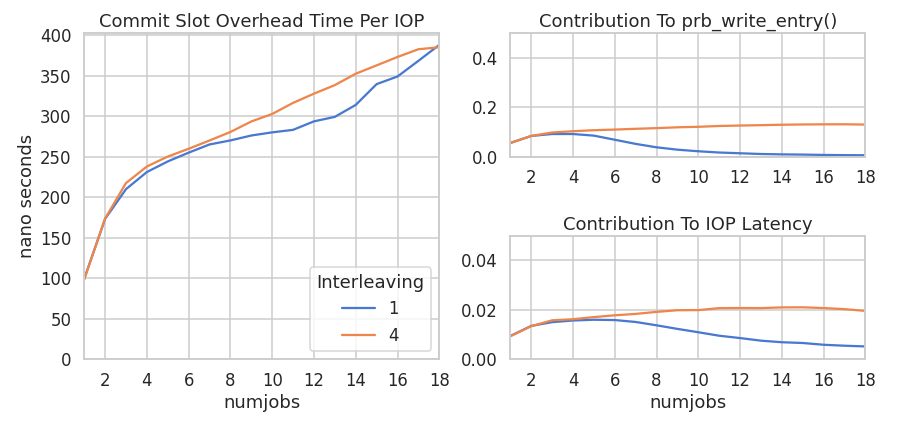
\includegraphics[width=\textwidth]{fig/evaluation/ncommitters_scalability__overhead}
    \caption{
        Overhead of the \textit{commit slot} for $24 = {\footnotesize \texttt{ncommitters}} > numjobs = 18$.
        Note the different y-axis scales.
        Also note that the relative latency contribution for the non-interleaved configuration only shrinks because the PMEM write time (not shown) grows significantly.}
    \label{fig:eval:ncommitters_scalability:overhead}
\end{figure}


We draw the following conclusion from the observations made above:
\begin{itemize}[noitemsep]
    \item The \textit{commit slot} mechanism successfully limits PMEM write time.
    \item The \textit{commit slots} mechanism's multi-core scalability is acceptable and contributes little relative overhead to each IOP compared to other ZFS components.
    \item Regarding the non-interleaved configuration (single Optane DIMM):
        \begin{itemize}
            \item Our 4k synchronous write workload is able to achieve peak performance with 400k IOPS as early as \lstinline{ncommitters=3}.
            \item Setting \lstinline{ncommitters=8} extends the peak to a plateau with regards to $numjobs$, but consumes $\frac{6500~\text{ns}}{3300~\text{ns}} = 1.96$ times more (on-CPU!) PMEM write time per IOP.
            \item Note that we use \lstinline{ncommitters=3} as the default configuration for ZIL-PMEM in all of the previous benchmarks.
                Our rationale is that an in-kernel filesystem should not waste CPU time on PMEM I/O because it is a system-wide OS service whose overall priority in the system is not known ahead of time.
                However, if the system's primary role is that of an NFS/SMB share, or that of a SCSI target (ZVOLs), it may be appropriate to allow more on-CPU waiting.
        \end{itemize}
    \item Regarding the four-way interleaved configuration (4 Optane DIMMs):
        \begin{itemize}
            \item The \textit{commit slot} mechanism is not useful for the observed range of $numjobs$ values.
            \item The reason is that ZIL-PMEM cannot saturate the Optane DIMMs' write bandwidth due to per-IOP overhead added by other components of ZFS.
            \item However, with ${\footnotesize\texttt{ncommitters}} > numjobs$, the overhead per IOP is negligible.
        \end{itemize}
\end{itemize}

\section{Discussion}

Storage stacks that we investigated but showed subpar perf:

\begin{itemize}
    \item xfs with separate log
    \item ext4 with separate log
\end{itemize}

Future work:

\begin{itemize}
    \item proof our write amplification claims (measure number of bytes of PMEM written as well as pmem write time, for all configurations. Needs instrumentation of pmem block device emulation.)
    \item ext4/xfs data journaling mode (ext4 has it, xfs not sure)
    \item xfs pmem-aware log (Christoph Hellwig has patches...)
    \item Scalability comparison of ZIL-LWB and ZIL-PMEM within the same dataset.
        Expectation: ZIL-PMEM's mutex eventually becomes the bottleneck, but likely still better than ZIL-LWB due to massive latency headroom.
\end{itemize}

\chapter{Summary}\label{ch:summary}

\section{Future Work}

\begin{description}
    \item[Evaluation Of Replay Performance]
    \item[Evaluation of Chunk Size] 

\end{description}

\backmatter

\chapter{Appendix}\label{ch:appendix}

\cleardoublepage
\phantomsection
\addcontentsline{toc}{chapter}{Bibliography}
\emergencystretch=1em
\printbibliography

\end{document}
